\documentclass[a4paper, openright, twoside]{report}
\usepackage[utf8]{inputenc}
\usepackage[main=american, german]{babel}
\usepackage{hyphenat}
\usepackage[activate={true,nocompatibility}, final, tracking=true, kerning=true, factor=1100, stretch=10, shrink=10]{microtype}
% Prevent hyphenization
\tolerance=1
\emergencystretch=\maxdimen
\hyphenpenalty=10000
\hbadness=10000

\usepackage[hmarginratio=1:1,textwidth=360pt,textheight=595.8pt]{geometry}
% Packages
\usepackage{import}

% Math
\newcommand\hmmax{0}
\newcommand\bmmax{0}
\usepackage{bm}
\usepackage{amsmath, amsfonts, amssymb, mathrsfs,extarrows}
\usepackage{upgreek}
\usepackage{commath}
\usepackage[retainorgcmds]{IEEEtrantools}
\usepackage{siunitx}
\usepackage{multirow}
\usepackage[widespace]{fourier}

% Tables
\usepackage{array}
\usepackage{caption}
\usepackage[figuresright]{rotating}
\usepackage{multirow}
\usepackage{makecell}
\usepackage{footnote}
\makesavenoteenv{tabular}

% Algorithm
\usepackage[chapter]{algorithm}
\usepackage{algpseudocode}

%% Citations
\usepackage[numbers]{natbib}
\bibliographystyle{humannat}
\citestyle{egu}
\usepackage[hyphens]{url}
% Bibliography showing in TOC
% \usepackage[nottoc,numbib]{tocbibind}
\usepackage[nottoc]{tocbibind}
\usepackage{scrlayer}
\DeclareNewLayer[
    foreground,
    %textarea,% use only the textarea
    contents={%
      \parbox[b][\layerheight][c]{\layerwidth}
        {\centering Page intentionally left blank.}%
    }
  ]{blankpage.fg}
\DeclarePageStyleByLayers{blank}{blankpage.fg}

% Control structures
\usepackage{ifthen}

% Listing
\usepackage{listings}
\usepackage{xcolor}
\usepackage{float}

% Review notes:
\usepackage{xargs}
\usepackage[textwidth=30mm,textsize=footnotesize]{todonotes} % to create comments (useful to your advisor!)
\newcommandx{\bpf}[2][1=]{\todo[linecolor=blue,backgroundcolor=blue!25,bordercolor=blue,#1]{#2}} % Bernardo notes

% Equation color background
\usepackage{mdframed}

\newmdenv[
    hidealllines=true,
    backgroundcolor=black!20,
    skipbelow=\baselineskip,
    skipabove=\baselineskip
]{highlight}

\newcounter{problem}[chapter]\setcounter{problem}{1}
\renewcommand{\theproblem}{\arabic{chapter}.\arabic{problem}}
\newenvironment{problem}[2][]{%
    \refstepcounter{problem}

    \mdfsetup{hidealllines=true,
    backgroundcolor=black!20,
    skipbelow=\baselineskip,
    skipabove=\baselineskip,
    frametitle={Problem~\theproblem~|~#1}}

\begin{mdframed}[]\relax}{%
\end{mdframed}}

% Enumeration
\usepackage{enumerate}


% Images
\usepackage[labelformat=simple]{subcaption}
\renewcommand\thesubfigure{(\alph{subfigure})}
\renewcommand\thesubtable{(\alph{subtable})}
\usepackage{graphicx}
\graphicspath{ {figures/} }
\usepackage{array}
\usepackage[section]{placeins}
\usepackage{color}
% \usepackage{subcaption}
% \usepackage{subfig}



% Images SVG
\usepackage{import}
\usepackage{xifthen}
\usepackage{pdfpages}
\usepackage{transparent}

\newcommand{\incfig}[1]{
    \def\svgwidth{0.3\columnwidth}
    \import{images/studies/minkowski/fundamental_forms_2D/}{#1.pdf_tex}}


% Floating environment for listings
\floatstyle{plain}
\newfloat{lstfloat}{htbp}{lop}[chapter]
\floatname{lstfloat}{Listing}
\def\lstfloatautorefname{Listing} % needed for hyperref/auroref

% Listing style
\definecolor{codegreen}{rgb}{0,0.6,0}
\definecolor{codegray}{rgb}{0.5,0.5,0.5}
\definecolor{codepurple}{rgb}{0.58,0,0.82}
\definecolor{backcolour}{rgb}{0.95,0.95,0.92}

\lstdefinestyle{mystyle}{
    backgroundcolor=\color{backcolour},
    commentstyle=\color{codegreen},
    keywordstyle=\color{blue},
    numberstyle=\tiny\color{codegray},
    stringstyle=\color{codepurple},
    basicstyle=\fontsize{7}{10}\selectfont,
    breakatwhitespace=false,
    breaklines=false,
    captionpos=b,
    keepspaces=true,
    numbers=left,
    numbersep=5pt,
    showspaces=false,
    showstringspaces=false,
    showtabs=false,
    tabsize=2
}

\lstset{style=mystyle}

\makeatletter
\newcommand*{\shifttext}[2]{%
  \settowidth{\@tempdima}{#2}%
  \makebox[\@tempdima]{\hspace*{#1}#2}%
}
\makeatother

\usepackage{pythonhighlight}

% Appendices
\usepackage[toc,page]{appendix}

% Headers and footers
\usepackage{fancyhdr}
% \renewcommand{\chaptermark}[1]{\markboth{\thechapter.\ #1}{}}
% \renewcommand{\sectionmark}[1]{\markright{\thesection.\ #1}}

% \fancypagestyle{plain}{
% \fancyhf{}
% \fancyhead{}% remove default header entries
% \fancyhead[RE]{a\textsc{\leftmark}}
% \fancyhead[LE]{\thepage}
% \fancyhead[LO]{\textsc{\rightmark}}
% \fancyhead[RO]{\thepage}
% \renewcommand{\headrulewidth}{0.1pt} }
% \pagestyle{plain}

\fancypagestyle{firststyle}
{
   \fancyhf{}
    \fancyhead{}% remove default header entries
   \fancyfoot[C]{Porto, September 2021}
   \renewcommand{\headrulewidth}{0pt}
\renewcommand{\footrulewidth}{0.1pt}
    \fancyfootoffset{-0.25\textwidth}
}

\pagestyle{fancy}
\fancyhf{}
\renewcommand{\chaptermark}[1]{\markboth{\thechapter.\ #1}{}}
\renewcommand{\sectionmark}[1]{\markright{\thesection.\ #1}}
\fancyhead{}% remove default header entries
\fancyhead[RE]{\nouppercase\leftmark}
\fancyhead[LE]{\thepage}
\fancyhead[LO]{\nouppercase\rightmark}
\fancyhead[RO]{\thepage}
\renewcommand{\headrulewidth}{0.1pt}

\newenvironment{dedication}
  {%\clearpage           % we want a new page          %% I commented this
   \thispagestyle{empty}% no header and footer
   \vspace*{\stretch{1}}% some space at the top
   \itshape             % the text is in italics
   \raggedleft          % flush to the right margin
  }
  {\par % end the paragraph
   \vspace{\stretch{3}} % space at bottom is three times that at the top
   \clearpage           % finish off the page
  }


% landscape
% \usepackage{lscape}
\usepackage{pdflscape}

%Custom FramedBox Environment
%%Loading 'float' package
\usepackage{float}
%%Customize 'boxed' float style (caption above the body)
\makeatletter
\newcommand\fs@boxedtop
 {\fs@boxed
  \def\@fs@mid{\vspace\abovecaptionskip\relax}%
  \let\@fs@iftopcapt\iftrue
 }
\makeatother
%%Defining float commands
\floatstyle{boxedtop}
\floatname{framedbox}{Box}
\newfloat{framedbox}{hbt}{lob}[chapter]

% Symbols
%% Differential Upright "d"
\newcommand{\ud}{\,\mathrm{d}}
%% Assemble operator
\DeclareMathOperator*{\assemble}{\text{\Large $ \mathsf{A} $}}
%% Matrices and vectors
\newcommand{\vect}[1]{\bm{#1}}
\newcommand{\mat}[1]{\bm{#1}}
\newcommand{\boldsf}[1]{\boldsymbol{\mathsf{#1}}}

\DeclareMathAlphabet{\pazocal}{OMS}{zplm}{m}{n}

\title{Numerical Methods}
\author{José Luís Passos Vila-Chã}
\date{May 2021}


\pagenumbering{roman}

%Hypertext marks
\usepackage[pdftitle={CFE_report},
			pdfauthor={JoseVila-Cha},
			pdfdisplaydoctitle=true,
			colorlinks=true,
			% Eletronic Version
             linkcolor=orange,
             citecolor=teal,
            % Print Version
            % linkcolor=black,
            % citecolor=black,
            bookmarks=true,
            bookmarksopen=false,
            bookmarksnumbered=true]{hyperref}

\usepackage[intoc]{nomencl}
\usepackage{xstring}
\usepackage{xpatch}
\patchcmd{\thenomenclature}
  {\leftmargin\labelwidth}
  {\leftmargin\labelwidth\itemindent 1em }
  {}{}

% Nomenclature

\makenomenclature
\renewcommand{\nomname}{Notation}
%% This code creates the groups
% -----------------------------------------
\usepackage{etoolbox}
\newcommand{\nomenclheader}[1]{%
  \item[\hspace*{-\itemindent}\bfseries\LARGE#1\vphantom{$\Bigg \vert $}]}
\renewcommand\nomgroup[1]{%
  \IfStrEqCase{#1}{%
   {A}{\nomenclheader{General abbreviations}}%      A - Acronyms
   {N}{\nomenclheader{General notation}}% R - Roman
   {O}{\nomenclheader{Operators and symbols}}% G - Greek
   {D}{\nomenclheader{Sets, domains and boundaries}}% G - Greek
   {S}{\nomenclheader{Subscripts and superscripts}}%  S - Superscripts
   {C}{\nomenclheader{Accents}}%    U - Subscripts
   {V}{\nomenclheader{Variables}}% X - Other Symbols
  }%
  \vspace{20pt}
}
\setlength{\nomitemsep}{-1pt}
% -----------------------------------------



\begin{document}
\begin{titlepage}
\thispagestyle{firststyle}
\begin{center}
   \begin{minipage}[c][10cm][l]{0.9\textwidth}

        \includegraphics[width=0.6\textwidth]{figures/university}

        \vspace{3.5cm}
        \huge
       \textbf{FFT-based Homogenization Methods}

       \vspace{1.5cm}
        \small
       \textit{Professor:}\\
       \normalsize
       Francisco Manuel Andrade Pires 	\\

       \vspace{0.5cm}


         \small
        \textit{Student:}\\
        \vspace{0.5cm}
       \normalsize
       \!José Luís Passos Vila-Chã
       \vspace{8cm}


        \centering
       \small
       Report presented under the scope of the\\ Doctoral Program in Mechanical Engineering

   \end{minipage}
   \end{center}
\end{titlepage}

\newpage\null\thispagestyle{blank}\newpage

\setcounter{tocdepth}{2}
\tableofcontents


\listoffigures


\listoftables

\newpage\null\thispagestyle{blank}\newpage

\pagenumbering{gobble}
\pagenumbering{arabic}
\pagestyle{fancy}
% \chapter{Introduction}

\section{Motivation}

The present work presents a partitioned thermomechanical solver.

The current work focuses on the developement of an implicit partitioned thermomechanical solver.

It presents a comprehensive dissertation on the thermodynamically consistent continuum mechanics.
It follows with the strictly mechanical problem, the strictly thermal problem and the full thermomechanical problem.
The corresponding intial value problems for the constitutive problem are introduced, as is the weak formulation of the relevant conservation and balance principles and their spatial and temporal discretization.

It follows a validation of the thermal solver.
The mechanical solver is not validated as it is part of the LINKS code used as the basis for the current developments.
Appropriate references are used in DIN 1992 and the NAFEMS benchmarks.
There is a good agreement between the numerical results and the references.

It follows a thorough investigation on the available approaches to solve coupled problems, with a special focus on thermomechanical problems.
A large sweep of the literature is performed, with the main classes of solution procdures being the monolithic approaches and the partitioned approaches.
The partioned approaches can be further divided into loosely coupled or explicit and strongly coupled or implicit.
Given the requirements put forth the most promising solution is determined to be a strongly coupled or implicit partitioned scheme.

Having performed this choice the following step is to understand the implicit methods available.
Recasting the problem as a system of nonlinear equations, where the residual is the difference bewteen the initial input and its output after applying the fixed-point.
This approach leads to the consideration of a large family of methods for the solution of nonlinear equations.
These are presented in detail for the solution of coupled multi-physics systems.
These are the fixed-point method, the underrelaxation method, the Aitken relaxation, the Broyden-like family of methods, the Newton-Krylov methods and the polynomial vector extrapolation methods, MPE and RRE, in cycling mode.

The validation of the thermomechanical solver and the implicit solution methodsm, as well as their comparison, is performed using to examples, whose results are present in the literature.
The expansion of an infinitely long thick-walled thermoelastic cylinder, and the necking of circular thermoelastoplastic bar.
The numerical results agree with the references provided confidence in the solution developed.
Regarding the comparison of the different implicit techniques, the best performing are the Broyden-like methods with \(\beta=-1\), Type I update and \(s=1\), corresponding to the good Broyden method, and \(s=2\).
These are both computationally efficient with few calls to the residual function and not very memory intensive.
The Aitken relaxation being the simplest and the least memory intensive also performs well.
The other methods considered, including the Newton-GMRES and the MPE in cycling mode, display a worse performance.
There is however a caveat regarding the Newton-Krylov methods regarding the possible use of global strategies such as line search given the accurate estimate for the Jacobian of the residual.
Moreover, it has been determined that most computationally demanding portion of the implicit partitioned schemes is the solution of the mechanical and thermal problems, with the manipulation concerning solely the coupling solver taking a very minute portion of the total computational time.



% The goal of computational micromechanics of materials is to establish a link between the mechanical response of two interacting scales in heterogeneous media, commonly referred to as the macro and micro-scale.
% It generally involves the numerical solution of the mechanical equilibrium of a periodic unit cell.
% It is a boundary value problem defined on a representative microscale sample that involves local constitutive laws, balance equations, and, most typically, periodic boundary conditions.
% The solution of this problem plays a pivotal role in bridging the two scales considered.
% The effective macroscopic response is then extracted from the solution of the local problem for a given macroscopic excitation.

Many processes use temperature.
There is a tigh connection between the thermal and the mechanical fields.

Having properly formulated the thermomechanical problem in a thermodynamically consistent way the problem can be solved using the Finite Element Method for the spatial discretizaiton and some other thing for the time discritization.

A thermal solver can be easily implemented to solve solely thermal problems.

To solve the fully thermal problem there are two common approaches, the monolithic approach where the balance equations considered after the discretization are the balance of mechanical and conservation of energy, and a partitioned approach, where the problems are solved speratly.
Whithin this scheme, one can still find loosley or explicit approach or a strongly coupled or implicit approach.
Both strategies can be found in the literature, having both their benifits and drawbacks.

% 
% For virtually all cases of practical relevance, the local problem must be solved approximately by discretizing the microstructure and the unknown microscopic fields.
% Such a unit-cell thereby provides a representative geometrical representation of the microstructure - which is often complex.
% An accurate representation of reality, therefore, necessitates a high-resolution numerical method, which remains efficient in three dimensions.
% The prevailing technique employed for this purpose is the Finite Element Method.
% However, the ever-increasing desire to use finely discretized unit cells, even in 3D, calls for more efficient methods.
% In particular, advances in experimental characterization of microstructures by high-resolution images triggers the need for efficient solvers that use these images directly as computational grids.
% A regular grid in combination with periodic boundary conditions naturally promotes solvers based on the Fast Fourier Transform (FFT) \citep{zeman_finite_2017, de_geus_finite_2017}.
% An attractive competitor to the Finite Element Method was developed by \cite{moulinec_fast_1994, moulinec_fft-based_1995}.
% It employs the Fast Fourier Transform (FFT) to obtain a significant gain in efficiency compared to Finite Elements, both in terms of speed and in terms of memory footprint.
% In the meantime extensions and different FFT-based approaches have been proposed.
% This work pretends to give an overview of the relevant literature on FFT-based homogenization procedures.
% 
% The improvements in efficiency obtained using the FFT-based procedures are of special relevance in the context of the data-driven design of materials, where the number of mechanical simulations needed to populate the database can be very large.
% Structural and material design is a highly iterative process where an optimal design for a chosen set of quantities of interest and a given set of restrictions is sought.
% For the particular case of material systems design, the high dimensionality of the engineering design space is striking when considering the overwhelming amount of possible combinations that lead to different materials \citep{bessa_framework_2017}, which often result in suboptimal and/or unexplored solutions.

\section{Computational Framework}

All the numerical simulations based on the Finite Element Method (FEM) are held in the in-house Fortran (IBM Mathematical Formula Translation System) program LINKS (Large Strain Implicit Non-linear Analysis of Solids Linking Scales), a multi-scale finite element code for implicit infinitesimal and finite strain analyses of hyperelastic and elastoplastic solids, that is continuously developed by the CM2S research group (Computational Multi-Scale Modeling of Solids and Structures) at the Faculty of Engineering of University of Porto.

In the present work, the author contributed to the addition of a suitable coupling environment for partitioned solution of coupled fields, as well as, a thermal solver based on the Finite Elements Method.

\section{Objectives}

The main goals of this work are:
\begin{itemize}
    \item To describe in a thermodynamically consitent way the thermomechanical problem;
    \item To develop and validate a thermal solver based on the Finite Element Method;
    \item To provide a thorough overview of the available methods for the solution of coupled problems, in particular, the thermomechanical problem;
    \item To validate the thermomechanical solver and compare the available strongly coupled partitioned strategies available in the literature.
\end{itemize}

\section{Document structure}

The remainder of this document is structured as follows:

\paragraph{Chapter \ref{ch:continuum_mechanics}}
In Chapter~\ref{ch:continuum_mechanics} provides a detailed description of a thermodynamical consistent continuum mechanics.
It includes the conservation and balance principles, dissipation inequalities and constitutive stuff.

\paragraph{Chapter \ref{ch:mechanical_problem}}
In Chapter~\ref{ch:mechanical_problem} presents the strictly mechanical problem including the intial value constitutive problem, the weak form of the momentum balance equation.
The mechanical intial value boundary value problem.
And discritize version using the Finite Element Method.

\paragraph{Chapter \ref{ch:thermal_problem}}
In Chapter~\ref{ch:thermal_problem} presents the strictly thermal problem including the constitutive law for the heat flux, the weak form of the energy equation, including its conduction.
The corresponding initial value boundary value problem.

\paragraph{Chapter \ref{ch:thermo_mechanical_problem}}
In Chapter~\ref{ch:thermo_mechanical_problem} presents the fully thermo-mechanical problem including the constitutive law for the heat flux, the weak form of the energy equation, including its conduction.
The corresponding initial value boundary value problem.

\paragraph{Chapter \ref{}}
In Chapter~\ref{} present the validation for the thermal solver using as references the \cite{DINEN1991_1_2} and \cite{NAFEMSbenchmarks}.
It includes both transient effects and boundary conditions such as natural convection and radiation.

\paragraph{Chapter \ref{}}
In Chapter~\ref{} presents an overview of the solution procedures for coupled problems.
It includes monolithic schemes, as well as, partitioned schemes, both explicit and implicit approaches.
An evaluation and discussion of the different methods is provided.

\paragraph{Chapter \ref{}}
In Chapter~\ref{} a thorough description of the available implicit methods is provided.
It rests on the recasting of the problem as a simple root-finding problem for a set of nonlinear equations.
The methods presented are the fixed-point method, the underrelaxation method, the Aitken relaxation, the Broyden-like family of methods, the Newton-Krylov methods, and the polynomial vection extrapolation methods in cycling mode.
Number of function of function evaluations, memory requirements, computational complexity and ease of implementation.

\paragraph{Chapter \ref{}}
In Chapter~\ref{} validation is provided for the thermomechanical solver and the implicit schemes explored in this work.
The efficiency of the best methods of each class of implicit methods described are compared as a function of the coupling strength.

\paragraph{Chapter \ref{chapter:conclusions}}
In Chapter~\ref{chapter:conclusions} the conclusions reached in this work are present and some future directions of research are suggested.


\newpage\null\thispagestyle{blank}\newpage

\include{thermomechanics}
\chapter{Continuum thermomechanics} \label{ch:continuum_mechanics}

This chapter covers the notions required to explain how a solid responds to thermal and mechanical loads under large deformations, including the conservation laws that guarantee mechanical equilibrium and energy conservation.
Additionally, the application of thermodynamics with internal variables is discussed along with the resulting inferences about the constitutive behavior of the material that makes up the solid.
These topics are broadly covered in the literature and here the approach used follows \cite{de_souza_neto_computational_2008},

\section{Kinematics of Deformation}

\subsection{Motion}

Let a deformable body $\mathscr{B}$ occupy an open region $\Omega_0$ of the tridimensional Euclidean space $\mathscr{E}$ with a regular boundary $\partial \Omega_0$ in its reference configuration.
Its motion, depicted in Figure \ref{}, is defined by a smooth one-to-one function
\begin{equation}
    \vect \varphi\colon \Omega\times \mathscr{R}\to \mathscr{E},
\end{equation}
mapping each material particle of coordinates $\vect X$ in the reference configuration to its position $\vect x$ in the deformed configuration, for a given instant of time $t$, as
\begin{highlight}
    \begin{equation}
        \vect x = \vect \varphi(\vect X, t)=\bm \varphi_t(\bm X).
    \end{equation}
\end{highlight}

\enlargethispage{\baselineskip}
Thus, the displacement field is defined as
\begin{equation}
    \vect u(\vect X, t) = \vect \varphi(\vect X, t) - \vect X,
\end{equation}
and, since the function that defines the motion is one-to-one, the reference configuration can be recovered as
\begin{equation}
    \vect X = \vect \varphi^{-1} (\vect x, t) = \vect x - \vect u(\vect \varphi^{-1}(\vect x, t),t),
\end{equation}
where $\vect \varphi^{-1}$ is the reference mapping function.

\begin{figure}
  \centering
  \includegraphics[width=.9\textwidth]{motion}
  \caption{Motion}
\label{fig:motion}
\end{figure}

\subsection{Material and spatial descriptions}

Dealing with finite deformations, the behavior of the body under analysis can be described with respect to the reference configuration, using the so-called material or Lagrangian description, or to the deformed configuration, using the so-called spatial or Eulerian description.

In the Lagrangian description any field, be it scalar, vectorial or tensorial defined over the body is expressed as a function of the reference configuration, $\vect X \in \Omega_0$.
On the other hand, the Eulerian descritpion of same field is done using the deformed configuration, $\vect x\in \Omega$.

As such let $\alpha(\vect x,t)$ be a spatial field and $\beta(\vect X, t)$ a material field.
Their material $\alpha_m$ and spatial $\beta_s$ desctiptions are given by
\begin{align}
    \alpha_m(\vect X, t) &=\alpha(\vect \varphi(\vect X, t),t),\\
    \beta_s(\vect x, t) &= \beta(\vect \varphi^{-1}(\vect x, t),t),
\end{align}
noting that any field associated with a motion of $\mathscr{B}$ can be expressed as a function of time and the point's position in the reference or deformed configuration.

The same distinction between material and spatial descriptions applies to operators such as the divergence and the gradient.
The spatial and material gradients, $\nabla$ and $\nabla_0$, respectively, are defined as
\begin{equation}
    \nabla \alpha = \frac{\partial}{\partial \vect x}\alpha(\vect x,t),\quad
    \nabla_0 \beta = \frac{\partial}{\partial \vect X}\beta (\vect X, t),
\end{equation}
where the derivatives are taken with respect to the spatial and reference configuration accordingly.

% \subsection{Velocity and acceleration}
%
% For solid dynamical problems, both the velocity and the acceleration corresponding to the motion \(\bm \varphi\) must be considered.
% The velocity is defined as
% \begin{gather}
%   \bm V = \frac{\partial \bm \varphi}{\partial t},\\
%   \bm v_t = \bm V_t \circ \bm \varphi_t^{-1},
% \end{gather}
% in the material and and spatial descriptions, respectively.
% See Figure~\ref{}.
% The formulas for the acceleration, again in both material and spatial descriptions, are
% \begin{gather}
%  \bm A = \frac{\partial \bm V}{\partial t},\\
%  \bm a = \bm A_t\circ \bm \varphi^{-1}_t.
% \end{gather}
% The spatial acceleration \(\bm a\) is related to the spatial velocity \(\bm v\) by
% \begin{equation}
%   \bm a = \dot{\bm v} = \frac{\partial \bm v}{\partial t} + \nabla \bm v\cdot \bm v.
% \end{equation}


\subsection{Deformation gradient}

The deformation gradient, a second order tensor denoted by $\mat F$, is defined as
\begin{highlight}
    \begin{equation}
            \mat F(\vect X,t)\equiv \nabla_0\vect\varphi(\vect X,t) =\frac{\partial \vect x}{\partial \vect X},
    \end{equation}
\end{highlight}
or, taking into account that
\begin{equation}
    \vect x = \vect X + \vect u(\vect X, t),
\end{equation}
it can be expressed as
\begin{equation}
    \mat F(\vect X, t) = \mat I + \nabla_0 \bm u.
\end{equation}

The deformation gradient relates the relative position between two neighboring material particles before and after deformation.
To see this let $\vect X$ be the coordinates of some material particle in the reference configuration and $\vect X + d\vect X$ the coordinates of some material particle in its neighborhood, their corresponding coordinates in the deformed configuration are given by
\begin{gather}
    \vect X = \vect x - \vect u(\vect X, t), \label{eq:mat_pos}\\
    \vect X + d\vect X = \vect x + d\vect x -\vect u(\vect X +d\vect X, t). \label{eq:mat_pos_delta}
\end{gather}
Subtracting Equation \eqref{eq:mat_pos} to Equation \eqref{eq:mat_pos_delta}, it is found that
\begin{align}
    d\vect X &= d\vect x +\vect u(\vect X, t)-\vect u(\vect X +d\vect X, t)\\
             &=(\mat I +\nabla_0 \vect u(\vect X, t))\; d\vect x\\
             &=\mat F\;d\vect x.
\end{align}

Due to this relation, it can be shown that the determinat of the deformation gradient has a physical meaning.
It is the local unit volume change, that is,
\begin{highlight}
\begin{equation}
   J\equiv \text{det}\;\mat F = \frac{dv}{dv_0}, \label{eq:det_grad_func}
\end{equation}
\end{highlight}
where $dv_0$ is an infinitesimal volume of the body in its reference configuration and $dv$ the infinitesimal volume after deformation.

\subsubsection{Isochoric/Volumetric decomposition}

Any deformation can be locally decomposed in volumetric and isochoric (or distortional) components.
From Equation \eqref{eq:det_grad_func} it can be gathered that an isochoric deformation is characterized by $J=1$.
As such, the deformation gradient can be decomposed as
\begin{equation}
    \mat F = \mat F_\text{iso} \mat F_\text{vol} = \mat F_\text{vol} \mat F_\text{iso},
\end{equation}
where the isochoric and columetric components are defined by
\begin{equation}
    \mat F_\text{iso} = (\text{det}\;\mat F)^{-\frac{1}{3}},\quad \mat F_\text{vol} = (\text{det}\;\mat F)^{\frac{1}{3}}\mat I.
\end{equation}

\subsubsection{Polar decomposition}

The deformation gradient can also be decomposed in rotation and stretch components, the so-called polar decomposition, defined as
\begin{highlight}
    \begin{equation}
        \mat F = \mat R\mat U = \mat V\mat R, \label{eq:polar_decomposition}
    \end{equation}
\end{highlight}
where $\mat R$ is the proper orthogonal rotation tensor and $\mat U$ and $\mat V$ are the symmetric positive right and left stretch tensors, respectively.

Equation \eqref{eq:polar_decomposition} has a physical interpretation with the right polar decomposition ($\mat F= \mat R\mat U$) corresponding to a stretch mapping followed by a rotation, and the left polar decomposition ($\mat F = \mat V\mat R$) corresponding to a rotation followed by a stretch mapping.
\
The right $\mat U$ and left $\mat V$ stretch tensors are related through the rotation matrix $\mat R$ as
\begin{equation}
    \mat V = \mat R\mat U\mat R^T,
\end{equation}
and can be obtained from deformation gradient by
\begin{highlight}
    \begin{equation}
        \mat C \equiv \mat U^2 = \mat F^T \mat F,\quad \mat B \equiv \mat V^2 = \mat F\mat F^T.,
    \end{equation}
\end{highlight}
where $\mat C$ and $\mat B$ are the right and left Cauchy-Green strain tensors.

Since $\mat U$ and $\mat V$ are symmetric tensors, they admit the spectral decomposition
\begin{equation}
    \mat U = \sum_{i=1}^3 \lambda_i \vect E_i^* \otimes \vect E_i^*,\quad \mat V = \sum_{i=1}^3 \lambda_i \vect e_i^*\otimes \vect e_i^*,
\end{equation}
where $\lambda_i$, $i=1,2,3,$ are the eigenvalues of both $\mat U$ and $\mat V$ and $\vect E_i^*$ and $\vect e_i^*$ are the respective eigenvectors.

The eigenvectors of left $\mat V$ and right $\mat U$ stretch tensors are related through
\begin{equation}
    \vect e_i^*= \mat R \vect E_i^*.
\end{equation}
forming two orthogonal bases.
These vectors define the Lagrangian and Eulerian principal directions, respectively, allowing for the expression of the local stretching from a material particle, associated with any deformation, as a superposition of stretches along the three mutual orthogonal directions.,

% \textcolor{red}{
% For solid dynamical problems, material time differentiation of the deformation and the strain measures need to be introduced. The first and second derivative of the displacement field \(u(X, t)\). li.e. the material velocity and acceleration, \(\dot{u}\) and \(\ddot{u}\), respectively, result in)
% where \((2.2)\) can be used to show that due to the constant initial position \(X\) )
% \[
% \hat{\boldsymbol{x}}(\boldsymbol{X}, t) \equiv \overline{\boldsymbol{u}}(\boldsymbol{X}, t)
% \]
% According to \((2.3)\), the material velocity gradient results in
% With the material gradient operator \(\operatorname{Grad}(\cdot)\). Equation \((2.23)\) can be reformulated, yielding the Ispatial velocity gradient
% and its symmetric part
% \[
% \begin{array}{c}
% \boldsymbol{L}=\dot{\boldsymbol{F}} \cdot \boldsymbol{F}^{-1} \\
% \boldsymbol{D}=\frac{1}{2}\left(\boldsymbol{L}+\boldsymbol{L}^{\top}\right)
% \end{array}
% \]
% The rate of the Green-Lagrange strain tensor results in the material strain rate tensor
% \[
% \dot{E}_{\mathrm{GL}}=\frac{1}{2} \dot{C}=\boldsymbol{F}^{\mathrm{T}} \cdot \boldsymbol{D} \cdot \boldsymbol{F}
% \]
% which can be expressed as pull-back of the symmetric spatial strain rate tensor \(D\). Via the Liederivative or Oldroyd-Lie derivative of the Euler-Almansi strain tensor \(\mathcal{L}_{t}\left[\boldsymbol{E}_{\mathrm{EA}}\right]\), which represents an objective material time derivative, a relation to the rate of the Euler-Almansi strain tensor is achieved as
% \[
% \mathcal{L}_{t}\left[\boldsymbol{E}_{\mathrm{EA}}\right]=\varphi\left[\frac{\mathrm{d}}{\mathrm{d} t}\left(\varphi^{-1}\left[\boldsymbol{E}_{\mathrm{EA}}\right]\right)\right]=\boldsymbol{D}=\boldsymbol{F}^{-\top} \cdot \dot{\boldsymbol{E}}_{\mathrm{GL}} \cdot \boldsymbol{F}^{-1}
% \]
% Moreover, the rate of volume changes is described by \(\dot{J}\) and can be expressed through
% \[
% \dot{J}=J \operatorname{tr} \boldsymbol{D}
% \]}


\section{Strain tensors}

In Continuum Mechanics there are two main families of strain tensors derived from the deformation gradient and used to describe the body deformation.
The Lagrange family strain tensors are defined as
\begin{equation}
    \mat E^{(m)} =\begin{cases} \displaystyle{\frac{1}{m} (\mat U^m - \mat I)},&\quad m\neq 0,\\[12pt] \ln(\mat U),& \quad m=0, \end{cases}
\end{equation} where $m$ is a real number, and likewise, the Euler family strain tensors are defined as
\begin{equation}
     \mat \varepsilon^{(m)} =\begin{cases} \displaystyle{\frac{1}{m} (\mat V^m - \mat I)},&\quad m\neq 0,\\[12pt] \ln(\mat V),& \quad m=0, \end{cases}
\end{equation}
where $m$ is also real number.

\enlargethispage{\baselineskip}
In particular, choosing $m=0$, one obtains the so-called material and spatial logarithmic strain tensors
\begin{highlight}[innertopmargin=-5pt]
    \begin{align}
        \mat E^{(0)} &\equiv \ln[\mat U] = \sum_{i=1}^3 \ln \lambda_i \vect E_i^*\otimes \vect E_i^*,\\
        \mat e^{(0)} &\equiv \ln [\mat V] = \sum_{i=1}^3 \ln \lambda_i \vect e_i^*\otimes \vect e_i^*.
    \end{align}
\end{highlight}


\section{Forces and stress measures}

The deformation of a body is intrinsically related to the forces acting on it.
These forces can be divided in two classes, from a purely mechanical point of view: volume (or body) forces, proportional to the mass contained in a volume element, as such measured in force per unit volume, and surface forces, acting on the surface of a volume element, measured as force per unit area.
Related to the latter is the concept of stress, that can be described mathematically by second order tensors with different definitions.

\subsubsection{Cauchy stress tensor}

According to Cauchy's theorem the relation between the so-called Cauchy stress vector, $\vect t(\vect x,\vect n)$, and the unitary outward vector normal to the deformed surface under analysis, $\vect n$, is linear and given by
\begin{highlight}
    \begin{equation}
        \vect t(\vect x,\vect n)\equiv \mat \sigma(\vect x)\vect n,
    \end{equation}
\end{highlight}
where $\mat \sigma$ is the second order Cauchy stress tensor.

The Cauchy stress vector is naturally associated with the deformed configured and thus, expressed in a spatial description and measured in force per unit deformed area.
It must also be noted that as a consequence of the balance of angular momentum, the Cauchy stress tensor is symmetric.

\subsubsection{First Piola-Kirchhoff stress tensor}

    The First Piola-Kirchhoff stress tensor, $\mat P$, can be regarded as the material counterpart of the Cauchy stress tensor, as it establishes a linear dependence between the stress vector $\vect t_0(\vect X,\vect m)$, measured in force per unit reference area, and the unitary outward vector normal to the undeformed surface under analysis, $\vect m$,
    \begin{equation}
        \vect t_0 = \mat P \vect m,
    \end{equation}
    which must related to the Cauchy stress vector by
    \begin{equation}
        \vect t_0 =\frac{\ud a}{\ud a_0} \vect t = \frac{\ud a}{\ud a_0} \mat \sigma \vect n,
    \end{equation}
    where $\ud a$ is the infinitesimal deformed area normal to the unitary vector $\vect n$ and $\ud a_0$ the corresponding undeformed are normal to $\vect m$.
    It can be shown that the relation between $da$ and $da_0$ is
    \begin{equation}
        \frac{da}{da_0}\vect n=J\mat F^{-T}\vect m,
    \end{equation}
    and substituting on the equation above motivates the following definition
    \begin{highlight}
        \begin{equation}
            \mat P \equiv J\mat \sigma \mat F^{-T}, \label{eq:def_piola}
        \end{equation}
    \end{highlight}
     where $J$ is the determinant of the deformation gradient $\mat F$ and $\mat \sigma$ is the Cauchy stress tensor.
     From Equation \eqref{eq:def_piola}, one gathers that, in general, the First Piola-Kirchhoff stress tensor is not symmetric.


\subsubsection{Kirchhoff stress tensor}

The Kirchhoff stress tensor, $\mat \tau$, is a widely used symmetric tensor, defined as
\begin{highlight}
    \begin{equation}
        \mat \tau \equiv J\mat \sigma.
    \end{equation}
\end{highlight}

\subsubsection{Deviatoric/Hydrostatic decomposition}

The Cauchy stress tensor, $\mat \sigma$, can split as
\begin{highlight}
    \begin{equation}
        \mat \sigma = \mat \sigma_d - p\mat I,
    \end{equation}
\end{highlight}
where $p$ is the hydrostatic pressure defined as
\begin{equation}
    p \equiv -\frac{1}{3}\text{tr}\;[\mat \sigma],
\end{equation}
and $\mat \sigma_d$ is the deviatoric stress defined as
\begin{equation}
    \sigma_d \equiv \mat \sigma - p\mat I.
\end{equation}

\section{Heat}

Heat flowing inside a body, entering or leaving it, often leads to temperature changes.
In Continuum Thermomechanics, heat is measured in power per unit surface.

\subsubsection{Heat flux vector}

According to Cauchy's theorem the relation between the heat flux across a surface, \(h(\bm x, \bm n)\), and the unitary outward normal to the deformed surface under analysis, \(\bm n\), is linear and given by
\begin{highlight}
  \begin{equation}
    h(\bm x, \bm n ) = -\bm q(\bm x)\cdot \bm n.
  \end{equation}
\end{highlight}
where \(\bm q\) is the heat flux vector.

\section{Fundamental conservation principles} \label{sec:fundamental_conservation_princ}

In Continuum Mechanics. there is a set of conservation principles and thermodynamic laws, that irrespective of the quantities used to describe the mechanical behavior of a body undergoing large deformations must always be satisfied.

\subsection{Principle of mass conservation}

The principle of mass conservation can be stated as
\begin{highlight}
    \begin{equation}
        \dot \rho + \rho\; \text{div}\; \dot{\bm u}=0,
    \end{equation}
\end{highlight}
    where $\rho$ is the material density measured in mass per unit deformed volume.

\subsection{Principle of linear momentum conservation}

The principle of linear momentum conservation can be stated in both material and spatial description.
In a spatial description it reads
\begin{highlight}
    \begin{equation}
        \begin{cases}
            \text{div}\;\mat \sigma + \vect b = \rho \ddot{\bm u},&\quad \forall\vect x\in \Omega,\\[12pt]
            \vect t = \mat \sigma \vect n,&\quad \forall\vect x\in\partial\Omega,
        \end{cases} \label{eq:material_equilibrium}
    \end{equation}
\end{highlight}
where $\vect b$ is the body forces field measured as per unit deformed volume.

One can also write the principle of linear momentum conservation in material coordinates, as
\begin{equation}
    \begin{cases}
        \text{div}_0\;\mat P + \vect b_0 = \rho_0 \ddot{\bm u},&\quad\forall \vect X\in \Omega_0,\\[12pt]
        \vect t_0 = \mat P \vect m,&\quad \forall\vect X\in\partial\Omega_0,
    \end{cases}\label{eq:spatial_equilibrium}
\end{equation}
where $\vect b_0$ is the body forces field, measured in force per unit undeformed volume, and $\rho_0$ is the material density, measured in mass per unit undeformed volume.
Both these quantities can be found from their spatial counterparts as
\begin{equation}
    \vect b_0 = J\vect b,\quad \rho_0 = J\rho.
\end{equation}
Take notice of the abuse of language regarding functions defined on the referece configuration \(\Omega_0\) and on the deformed configuration \(\Omega\).
The same symbol, \(f\), is used for a function \(f\) defined on \(\Omega\) and the function \(f\circ \bm\varphi\) defined on \(\Omega_0\).

Equations \eqref{eq:material_equilibrium} and \eqref{eq:spatial_equilibrium} are the so-called strong, point-wise or local equilibrium equations, as they enforce the mechanical equilibrium at every material particle of the body.

\subsection{First principle of thermodynamics} \label{sec:first_principle_thermo}

Let \(e\) be the internal energy per unit mass, \(r\) the heat supply per unit mass and \(\bm q\) the heat flux, then the first principle of thermodynamics pertaining to the balance of energy can be written in the spatial description as
\begin{highlight}
\begin{equation} \label{eq:first_principle_thermo}
  \begin{cases}
    \rho\dot e = \mat \sigma\;:\;\mat D + \rho r -\text{div}\;\vect q,\quad &\forall \bm x\in\Omega,\\
    \bm t = \bm \sigma \bm n,\quad &\forall \bm x\in \partial \Omega,\\
    h = \bm q \cdot \bm n,\quad &\forall \bm x\in \partial \Omega.
  \end{cases}
\end{equation}
\end{highlight}
The second order tensor $\mat D$ denotes a strain rate measure, such that the double contraction $\mat \sigma\colon\mat D$ represents the stress power per unit volume in the deformed configuration of body.
In material coordinates, it reads
\begin{equation}
  \begin{cases}
 \rho_0 \dot e = \bm P :\dot{\bm F} + \rho_0 r -\operatorname{div}_0 \bm q_0,\quad& \forall \bm X\in\Omega_0,\\
 \bm t_0 = \bm P\bm m,\quad&\forall \bm X\in\partial \Omega_0,\\
 h_0 = \bm q_0\cdot\bm m,\quad&\forall \bm X\in\partial \Omega_0,
  \end{cases}
\end{equation}
where \(\bm q_0\) is the Piola transformation of \(\bm q\), i.e.,
\begin{equation}
  \bm q_0 = J \bm F^{-T} \bm q,
\end{equation}
and
\begin{equation}
  h_0 = J h.
\end{equation}


\subsection{Second principle of thermodynamics}

The local entropy balance can written as
\begin{equation}
  \rho \dot s = -\operatorname{div}\left[\frac{\bm q}{\theta}\right] + \frac{\rho r}{\theta} + \hat{s},
\end{equation}
where \(\hat{s}\) is the entropy production.
The second principle of thermodynamics postulates that the changes in the entropy in the universe can never be negative, which is mathematically expressed by
\begin{equation}
  \hat s \geq 0,
\end{equation}
yielding
\begin{equation}
    \rho\dot s +\text{div}\left[\frac{\vect q}{\theta}\right] -\frac{\rho r}{\theta} \geq 0,
\end{equation}
   where $\theta$ and $s$ are the temperature and specific entropy fields respectively.
In a material description, it reads
\begin{equation}
  \rho_0 \dot s + \operatorname{div}_0 \left[\frac{\bm q_0}{\theta}\right] - \frac{\rho_0 r}{\theta} \geq 0.
\end{equation}

\subsection{Clausius-Duhem inequality}

Combining the first and second thermodynamic principles yields
\begin{equation}
    \rho\dot s + \text{div}\;\left[\frac{\vect q}{\theta}\right] -\frac{1}{\theta}(\rho\dot e -\mat\sigma\;:\bm D\; +\text{div}\;\vect q)\geq 0,
\end{equation}

From the definition of the specific Helmholtz free energy
\begin{highlight}
\begin{equation} \label{eq:def_helmholtz_free_energy}
    \psi \equiv e -\theta s,
\end{equation}
\end{highlight}
and defining the temperature field gradient as $\bm g=\nabla \theta$, it is possible to establish the so-called Clausius-Duhem inequality in the spatial description as
\begin{highlight}
    \begin{equation}
        \underbrace{\mat \sigma:\mat D - \rho\left(\dot \psi +s\dot \theta\right)}_{\pazocal D_\text{int}} \underbrace{-\frac{1}{\theta}\vect q\cdot \vect g }_{\pazocal D_\text{cond}}\geq 0, \label{eq:clasius_duhem_eq}
    \end{equation}
\end{highlight}
where the identity
\begin{equation}
    \text{div}\;\left[\frac{\vect q}{\theta}\right] =\frac{1}{\theta}\text{div}\;\vect q -\frac{1}{\theta^2}\vect q\cdot \nabla \theta.
\end{equation}
is used.

From a physical point of view, the Clausius-Duhem inequality states that the energy dissipation per unit deformed volume is always non-negative.
Moreover the terms in the inequalitiy can be splited into the internal dissipation \(\pazocal D_\text{int}\) and the dissipation due to heat conduction \(\pazocal D_\text{cond}\).
From
\begin{equation}
\hat s = \bm \sigma :\bm D - \rho \left(\dot \psi  +s \dot \theta\right) -\frac{1}{\theta}\bm q\cdot\bm g,
\end{equation}
assuming that the process leads to an uniform temperature distribution, yields for the internal dissipation \(\pazocal D_\text{int}\),
\begin{equation} \label{eq:def_int_dissipation}
\pazocal D_\text{int} = \hat{s}|_{\text{$\theta$ uniform} }= \bm \sigma:\bm D - \rho \left(\dot \psi + s \dot \theta\right),
\end{equation}
since conduction is excluded.
If on the other hand, only conduction effects are retained, the dissipation due to conduction, \(\pazocal D_\text{cond}\), is obtained as
\begin{equation} \label{eq:dissipation_conduction}
\pazocal D_\text{cond} = - \frac{1}{\theta} \bm q\cdot \bm g.
\end{equation}

Equation \eqref{eq:clasius_duhem_eq} can also be written as
\begin{equation}
  \bm P\colon\dot{\bm F} - \rho_0(\dot\psi + s\dot \theta) - \frac{1}{\theta}\bm q_0\cdot \bm g_0 \geq 0,
\end{equation}
where \(\bm g_0 = \nabla_0 \theta\), aplying the Piola transformation, and as
\begin{equation}
    \mat \tau\;:\;\mat D -\rho_0\left(\dot\psi + s\dot \theta\right) -\frac{J}{\theta}\vect q\cdot \vect g \geq 0,
\end{equation}
multiplying it by $J$ and attending to the definition of the Kirchhoff stress tensor, where the left hand side represents now the energy dissipation per unit reference volume.


\section{Thermomechanical constitutive initial value problem} \label{sec:thermomechanical_constitutive}

In Continuum Mechanics, a constitutive model is a set of equations, also called constitutive equations, establishing the stress-strain relation for some material.
Before going further, it is important to define a thermokinetic process of a body $\mathscr{B}$ as
\begin{highlight}
    \begin{equation}
        \text{thermokinetic process:}\quad\{\vect \varphi(\vect X, t), \theta(\vect X, t)\},
    \end{equation}
\end{highlight}
and a calordynamic process of $\mathscr{B}$ as
\begin{highlight}
    \begin{equation}
        \text{calorodynamic process:}\quad \{\mat \sigma(\vect X, t), e(\vect X, t), s(\vect X, t), r(\vect X, t), \vect b(\vect X,t), \vect q(\vect X, t)\},
    \end{equation}
\end{highlight}
which satisfies the fundamental conservation principles previously introduced.

It is also important to note that any constitutive model must satisfy a set of constitutive axioms, explained  in detail in \cite{de_souza_neto_computational_2008}.
As these are too general to be used directly in practice, a particular case of the general history functional-based constitutive theory based on the thermodynamics with internal variables approach is used.

\subsection{Thermodynamics with internal variables}

The values of $\mat \sigma$, $\psi$, $s$ and $\vect q$ at a material particle define its thermodynamic state, assuming \(\bm b\) follows from the balance of linear momentum and \(r\) from the energy balance equation.
In thermodynamics with interval variables approach, that thermodynamic state is assumed to be completely defined by the instantaneous values of a finite number of state variables
\begin{equation}
    \{\mat F, \theta, \vect g, \vect \alpha\}.
\end{equation}
at a given instant of the calorodynamic process, where
\begin{equation}
    \vect \alpha = \{\alpha_k\}
\end{equation}
is a set of internal variables, scalar or tensorial in nature, associated with dissipative mechanisms.
As such, the accuracy of the constitutive model depends strongly on the appropriate choice of internal variables, as these contain the relevant information about the thermodynamical history of the material.

Accordingly, the specific Helmholtz free energy is postulated to follow
\begin{highlight}
    \begin{equation}
        \psi = \psi(\mat F, \theta, \vect \alpha).
    \end{equation}
\end{highlight}
To find the constitutive equations for the stress tensor and the entropy, one can substitute
\begin{equation}
    \dot \psi = \frac{\partial \psi}{\partial \mat F}:\dot{\mat F} + \frac{\partial \psi}{\partial \theta}\dot \theta + \frac{\partial \psi}{\partial \alpha_k}\dot \alpha_k,
\end{equation}
found from the chain rule, into the Clausius-Duhem equation, Equation \eqref{eq:clasius_duhem_eq}, obtaining
\begin{equation}
    \left(\mat \sigma \mat F^{-T} -\rho\frac{\partial \psi}{\partial \mat F}\right):\dot{\mat F} -\rho \left(s+\frac{\partial \psi}{\partial \theta}\right)\dot \theta - \rho \frac{\partial \psi}{\partial \alpha_k}\dot\alpha_k - \frac{1}{\theta}\vect q \cdot \vect g\geq 0,\label{eq:clausius_duhem_energy}
\end{equation}
where the velocity gradient was adopted to set the work conjugacy as
\begin{equation}
    \mat \sigma :\mat D = \mat \sigma :\mat L = \mat \sigma :\dot{\mat F}\mat F^{-1} = \mat \sigma \mat F^{-T}:\mat F.
\end{equation}

Since the Clausius-Duhem inequality must hold for any thermokinetic process and so remain valid for any set $\{\dot{\mat F}(t),\dot \theta(t)\}$, the Cauchy stress and entropy constitutive equations must be
\begin{highlight}[innertopmargin=-5pt]
    \begin{gather}
        \mat \sigma = \rho \frac{\partial \psi}{\partial \mat F}\mat F^T, \label{eq:const_signa}\\
        s = -\frac{\partial \psi}{\partial \theta}.
    \end{gather}
\end{highlight}

It is also possible to write the constitutive equations for the Kirchhoff stress tensor as
\begin{equation}
    \mat \tau = J\rho \frac{\partial \psi}{\partial \mat F}\mat F^T,
\end{equation}
multiplying Equation \eqref{eq:const_signa} by $J$, and the first Piola-Kirchhoff stress tensor as
\begin{equation}
    \mat P = \rho_0 \frac{\partial \psi}{\partial \mat F}
\end{equation}
multiplying Equation \eqref{eq:clausius_duhem_energy} also by $J$.

For each internal variable $\alpha_k$ of the set $\alpha$ of internal variables, the conjugate thermodynamical forces are defined to be
\begin{equation}
    A_k\equiv \rho_0 \frac{\partial \psi}{\partial \alpha_k},
\end{equation}
so that the Clausius-Duhem equation can be written in a reduced form as
\begin{highlight}
    \begin{equation}
        -\bm A*\dot{\vect \alpha} - \frac{J}{\theta}\vect q\cdot \vect g\geq 0,
    \end{equation}
\end{highlight}
where $\vect A$ is the set of conjugate thermodynamical forces and \(*\) denotes the appropriate product operation.

To completely define the constitutive model, one still needs to postulate the constitutive equations for the flux variables $\dot{\vect \alpha}$ and $\frac{1}{\theta}\vect q$.
These are given by
\begin{highlight}[innertopmargin=-5pt]
            \begin{gather}     \dot{\vect \alpha} = f(\mat F, \theta, \vect g, \vect \alpha),\\      \frac{1}{\theta}\vect q = g(\mat F, \theta, \vect g, \vect \alpha).
            \end{gather}
\end{highlight}

A sufficient condition for the previous constitutive functions to satisfy the Clausius-Duhem inequality is the hypothesis of normal dissipativity, whereby one defines the constitutive functions for the flux variables as
\begin{highlight}
    \begin{equation}
        \dot \alpha_k = -\frac{\partial \Xi}{\partial A_k},\quad \frac{1}{\theta}\vect q = -\frac{\partial \Xi}{\partial \vect g},
    \end{equation}
\end{highlight}
where the dissipation potential is
\begin{equation}
    \Xi= \Xi(\mat A, \vect g; \mat F, \theta, \vect \alpha),
\end{equation}
a convex function with respect to each $A_k$ and $\vect g$, and zero valued at the origin, $\{\vect A,\vect g\}=\{\vect 0,\vect 0\}$.
Note that in the previous definition the state variables appear only as parameters.

\newpage\null\thispagestyle{blank}\newpage

\chapter{Mechanical problem}

\subsection{Mechanical constitutive initial value problem}

In the purely mechanical case, with all the quantities related to the thermal domain can removed, a constitutive model based on internal variables can be established by the following set of equations
    \begin{gather}
        \mat P = \rho_0 \frac{\partial \psi}{\partial \mat F},\\
        \psi = \psi(\mat F,\mat \alpha),\\
        \dot{\vect \alpha} = f(\mat F, \vect \alpha).
    \end{gather}
    Thus, the spatial mechanical constitutive initial value problem can be stated as follows
    \begin{problem}[Spatial mechanical constitutive intial value problem.]
    GGiven the initial values of the internal variables, $\vect \alpha(t_0)$, and the history of the deformation gradient
    \begin{equation}
        \mat F(t),\quad t\in[t_0,t_\text{end}],
    \end{equation}
    find the functions for $\mat sigma(t)$ and $\vect \alpha(t)$ such that the constitutive equations
    \begin{gather}
        \mat \sigma = \rho \frac{\partial \psi}{\partial \mat F} \mat F^T,\\
        \psi = \psi(\mat F, \vect \alpha),\\
        \dot{\vect \alpha} = f(\mat F, \vect \alpha).
    \end{gather}
    are satisfied for every $t\in [t_0, t_\text{end}]$.
    \end{problem}

Likewise, in a material description it can be stated as
    \begin{problem}[Material mechanical constitutive intial value problem.]
    GGiven the initial values of the internal variables, $\vect \alpha(t_0)$, and the history of the deformation gradient
    \begin{equation}
        \mat F(t),\quad t\in[t_0,t_\text{end}],
    \end{equation}
    find the functions for $\mat P(t)$ and $\vect \alpha(t)$ such that the constitutive equations
    \begin{gather}
        \mat P = \rho_0 \frac{\partial \psi}{\partial \mat F},\\
        \psi = \psi(\mat F, \vect \alpha),\\
        \dot{\vect \alpha} = f(\mat F, \vect \alpha).
    \end{gather}
    are satisfied for every $t\in [t_0, t_\text{end}]$.
    \end{problem}
\enlargethispage{3\baselineskip}
It is now possible to pose the quasi-static mechanical constitutive initial value problem in its weak form.
To do it one assumes that a body $\mathscr{B}$ is made from a generic material, characterized by a given constitutive models, whose internal variables are known at the initial time, as presented in Figure \ref{}.
In addition, it is assumed that the interior of the body was subjected to a prescribed history of body forces, $\vect b(\vec X, t)$, $t\in[t_0, t_\text{end}$, and to the following boundary conditions:
\begin{itemize}
    \item \textbf{Natural (or Neumann) boundary condition:}
    The boundary portion $\Omega_\text{traction, 0}$ of $\mathscr{B}$ is subjected to a prescribed history of traction forces, $\vect t_\text{presc}(\vect X, t)$, $\vect X\in \partial \Omega_\text{traction,0}$, $t\in[t_0, t_\text{end}]$,\\
    \item \textbf{Essential (or Dirichlet) boundary condition:}
    The boundary portion $\Omega_\text{motion, 0}$ of $\mathscr{B}$ is subjected to a prescribed displacement field history, $\vect u_\text{presc}(\vect X, t)$, such that $$\vect \varphi(\vect X, t) = \vect X + \vect u_\text{presc}(\vect X, t),\quad \vect X\in \partial\Omega_\text{motion, 0},\quad t\in[t_0, t_\text{end}].$$
\end{itemize}

It is also convenient to define the set of kinematically admissible displacements of $\mathscr{B}$ as the set of all sufficiently regular displacement functions tha satisfy the essential boundary condition \citep{de2011computational},
\begin{highlight}[innertopmargin=-5pt]
    \begin{multline}
        \mathscr{K}\equiv \{\vect u:\Omega\times \mathscr{R}\to \mathscr{U}\;|\;\vect u(\vect X,t) = \vect u_\text{presc} (\vect X,t),\\ \vect X\in\partial \Omega_\text{motion,0},\quad t\in [t_0,t_\text{end}]\}.\quad
    \end{multline}
\end{highlight}

So the weak form of the quasi-static mechanical constitutive initial boundary value problem can be stated in a spatial description as follows
\begin{problem}[Spatial quasi-static mechanical initial BVP.]
    Find a kinematically admissible displacement function, $\vect u\in \mathscr{K}$, such that for every $t\in [t_0,t_\text{end}]$, the body $\mathscr{B}$ is in equilibrium as stated by the Virtual Work Principle
        \begin{equation}
        \int_\Omega [\mat \sigma:\nabla \vect \eta - \vect b\cdot \vect \eta]\ud v - \int_{\partial\Omega} \vect t\cdot \vect \eta\ud a = 0,\quad \forall \vect \eta \in \mathscr{V},
    \end{equation}
    where the space of virtual displacements at time $t$ is defined by
    \begin{equation}
        \mathscr{V} \equiv \left\{\vect \eta:\Omega\to \mathscr{U}\;|\;\vect \eta = \vect 0\quad \text{in}\quad \partial\Omega_\text{motion,0}\right\},
    \end{equation}
    and at each point of $\mathscr{B}$, the Cauchy stress tensor is the solution of spatial mechanical constitutive initial values problem.
\end{problem}
and in the material description as
\begin{problem}[Material quasi-static mechanical initial BVP.]
    Find a kinematically admissible displacement function, $\vect u\in \mathscr{K}$, such that for every $t\in [t_0,t_\text{end}]$, the body $\mathscr{B}$ is in equilibrium as stated by the Virtual Work Principle
        \begin{equation}
        \int_{\Omega_0} [\mat P:\nabla_0 \vect \eta - \vect b_0\cdot \vect \eta]\ud v - \int_{\partial\Omega_0} \vect t_0\cdot \vect \eta\ud a = 0,\quad \forall \vect \eta \in \mathscr{V},
    \end{equation}
    where the space of virtual displacements at time $t$ is defined by
    \begin{equation}
        \mathscr{V} \equiv \left\{\vect \eta:\Omega_0\to \mathscr{U}\;|\;\vect \eta = \vect 0\quad \text{in}\quad \partial\Omega_\text{motion,0}\right\},
    \end{equation}
    and at each point of $\mathscr{B}$, the First Piola-Kirchhoff stress tensor is the solution of material mechanical constitutive initial values problem.
\end{problem}

\newpage
\section{Time descretization} \label{sec:time_discretization}

Given a generic path-dependent model, i.e. a model in which the stress state does not depend only on the instantaneous deformation state but also on the deformation history, the solution of the constitutive initial value problem for a given set of initial conditions is usually not known for complex strain paths $\mat F(t)$.
Thus, there is a need to use an appropriate numerical algorithm for integration of the rate constitutive equations.

In general, the algorithms for the integration of rate constitutive equations are obtained adopting some kind of time (or pseudo-time) discretisation along with some hypothesis on the deformation path between adjacent time stations.

In the present document, it is adopted an algorithm based on approximated incremental constitutive functions.
Attending to the mechanical constitutive initial boundary value problem and considering the time increment $[t_n, t_{n+1}]$, this approach is comprised by the following two requeriments:
\begin{itemize}
    \item \textbf{Cauchy and First Piola-Kirchhoff stress tensors.}   Considering a time increment $[t_n, t_{n+1}]$ and given the set $\vect \alpha_n$ of internal variables at $t_n$, the deformation gradient $\mat F_{n+1}$ at time $t_{n+1}$ determines the stress $\mat \sigma_{n+1}$ uniquely through
    \begin{highlight}
        \begin{equation}
            \mat \sigma_{n+1} = \hat{\mat \sigma}(\vect \alpha_n, \mat F_{n+1}), \label{eq:incremental_stress}
        \end{equation}
    \end{highlight}
    where $\hat{\vect \sigma}$ is the incremental constitutive function for the Cauchy stress tensor.

    Similarly, the First Piola-Kirchhoff stress tensor $\mat P_{n+1}$ must be uniquely determined by the prescribed deformation gradient $\mat F_{n+1}$ prescribed at $t_{n+1}$ as
    \begin{equation}
        \mat P_{n+1} = \hat{\mat P}(\mat F_{n+1}, \mat \alpha_n),
    \end{equation}
    where $\hat{\mat P}$ is the incremental constitutive function for the First Piola-Kirchhoff stress tensor.
    \item \textbf{Set of internal variables.} Assuming that the set of internal variables $\vect \alpha_n$ is known at $t_n$, the set of internal variables must be uniquely determined by the prescribed deformationgradient $\mat F_{n+1}$ prescribed at $t_{n+1}$ as
    \begin{highlight}
        \begin{equation}
             \vect \alpha_{n+1} =\hat{\vect \alpha}(\vect \alpha_n, \mat F_{n+1}), \label{eq:incremental_flux}
        \end{equation}
    \end{highlight}
    where $\hat{\vect \alpha}$ is the incremental constitutive function for the set of internal variables.
\end{itemize}

Generally, the numerical constitutive laws are nonlinear and path-independent within one increment, that is, within each increment, $\mat \sigma_{n+1}$ and $\vect \alpha_{n+1}$ are  functions of $\mat F_{n+1}$ alone with the argument $\vect \alpha_n$ constant within the same time interval.

Making use of the aforementioned time discretization, the weak form of the quasi-static mechanical constitutive initial boundary value problem can then be stated in the spatial description as
\begin{problem}[Spatial incremental quasi-static mechanical initial BVP.]
    GGiven the set of internal variables $\vect \alpha_n$ at $t_n$, the prescribed body and traction force fields $\vect b_{n+1}$ and $\vect t_{n+1}$ at $t_{n+1}$, and the prescribed deformating gradient $\mat F_{n+1}$ at $t_{n+1}$, find the kinematically admissible displacement field $\vect u_{n+1}\in\mathscr{K}_{n+1}$ such that the body $\mathscr{B}$ is in equilibrium as stated by the virtual Work Principle
            \begin{equation}
        \int_{\Omega_{n+1}} [\hat{\mat \sigma}(\mat F_{n+1}, \vect \alpha_n):\nabla \vect \eta - \vect b_{n+1}\cdot \vect \eta]\ud v - \int_{\partial\Omega_{n+1}} \vect t_{n+1}\cdot \vect \eta\ud a = 0,\quad \forall \vect \eta \in \mathscr{V},
    \end{equation}
    where the space of kinematically admissible displacement fields $\mathscr{K}_{n+1}$ is defined by
    \begin{equation}
            \mathscr{K}_{n+1}\equiv \{\vect u:\Omega\times \mathscr{R}\to \mathscr{U}\;|\;\vect u_{n+1}(\vect X) = \vect u_\text{presc,$n+1$}(\vect X),\;\vect X\in\partial \Omega_\text{motion,0}\}.
    \end{equation}
\end{problem}
and in the material description as
\begin{problem}[Material incremental quasi-static mechanical initial BVP.]
    GGiven the set of internal variables $\vect \alpha_n$ at $t_n$, the prescribed body and traction force fields $\vect b_{0,n+1}$ and $\vect t_{0,n+1}$ at $t_{n+1}$, and the prescribed deformating gradient $\mat F_{n+1}$ at $t_{n+1}$, find the kinematically admissible displacement field $\vect u_{n+1}\in\mathscr{K}_{n+1}$ such that the body $\mathscr{B}$ is in equilibrium as stated by the virtual Work Principle
            \begin{equation}
        \int_{\Omega_{n+1}} [\hat{\mat P}(\mat F_{n+1}, \vect \alpha_n):\nabla_0 \vect \eta - \vect b_{0,n+1}\cdot \vect \eta]\ud v - \int_{\partial\Omega_{n+1}} \vect t_{0,n+1}\cdot \vect \eta\ud a = 0,\quad \forall \vect \eta \in \mathscr{V},
    \end{equation}
    where the space of kinematically admissible displacement fields $\mathscr{K}_{n+1}$ is defined by
    \begin{equation}
            \mathscr{K}_{n+1}\equiv \{\vect u:\Omega\times \mathscr{R}\to \mathscr{U}\;|\;\vect u_{n+1}(\vect X) = \vect u_\text{presc,$n+1$}(\vect X),\;\vect X\in\partial \Omega_\text{motion,0}\}.
    \end{equation}
\end{problem}

\section{Finite Element Method} \label{sec:fem}

With the incremental weak form of the quasi-static mechanical constitutive initial boundary value problem now established, an approximated solution can be found making use of the Finite Elment Method.

\subsection{Finite element concept}

The first in the Finite Element method is to discretize the continuum domain $\Omega$ in a finite set of $n_\text{elem}$ mutually exclusive subdomains called finite elements $\Omega^{(e)}$.
The discretized domain, $^h\Omega$, is therefore an approximation to the continuum domain expressed by
\begin{equation}
    \Omega \approx ^h\Omega \equiv \bigcup_{e=1}^{n_\text{elem}}\Omega^{(e)}.
\end{equation}
The space of virtual displacements $\mathscr{V}$ as well as the space of kinematically admissible displacement fields $\mathscr{K}$ are also discretized in the same, with their discretized forms denoted by $^h\mathscr{V}$ and $^h\mathscr{K}$.

\subsection{Interpolation functions}

Let $e$ be a generic finite element with $n_\text{nodes}$ nodes, where each node $i$ of coordinates $\vect x^i$ is associated with an interpolation function $N_i^{(e)}$.
These interpolation functions are often called shape functions and perform the required filed interpolations inside the element domain $\Omega^{(e)}$.

Letting $a(\vect x)$ be a generic field defined over $\Omega^{(e)}$, its interpolation at any point $\vect x$ inside the element is defined by the element shape functions as
\begin{highlight}
    \begin{equation}
        a(\vect x) \approx ^ha(\vect x) \equiv \sum_{i=1}^{n_\text{nodes}} a(\vect x_i) N_i^{(e)}(\vect x).
    \end{equation}
\end{highlight}
If instead $a(\vect x)$ is instead a generic field defined over the global domain $\Omega$, the interpolation of $a(\vect x)$ at any point $\vect x$ is defined by the global shape functions as
\begin{highlight}
    \begin{equation}
        a(\vect x) \approx ^h a(\vect x) \equiv \sum_{i=1}^{n_\text{points}} a(\vect x_i) N_i^g(\vect x), \label{eq:interpol_global}
    \end{equation}
\end{highlight}
where $n_\text{points}$ is the total number of nodes of the finite element mesh.
The discretized spaces $^h \mathscr{V}$ and $^h\mathscr{K}$ can now be defined as
\begin{align}
    ^h \mathscr{K}&\equiv \Big\{\vphantom{|}^h\vect u(\vect x) = \sum_{i=1}^{n_\text{points}} \vect u(\vect x_i) N_i^g(\vect x)\;|\; \vect u(\vect x_i) = \vect u_\text{presc}(\vect x_i)\quad\text{if $\vect x_i\in \partial\Omega_\text{motion,0}$}  \Big\},\\
    ^h\mathscr{V}&\equiv \Big\{\vphantom{|}^h\vect \eta(\vect x) = \sum_{i=1}^{n_\text{points} } \vect \eta(\vect x_i) N_i^g(\vect x)\;|\;\vect \eta(\vect x_i)=\vect 0\quad\text{if $\vect x_i\in \partial\Omega_\text{motion,0}$}   \Big\}
\end{align}

\subsection{Interpolation matrix and discrete gradient operators}

The global shape functions can be conveniently assembled in the so-called global interpolation matrix as
\begin{equation}
    \mat N^g(\vect x) \equiv \left[\text{diag}[N_1^g(\vect x)]\; \text{diag}[N_2^g(\vect x)]\;\cdots\; \text{diag}[N_{n_\text{points}}^g(\vect x)]\right],
\end{equation}
where $\text{diag}[N_i^g]$ is a diagonal matriz $n_\text{dim} \times n_\text{dim}$
\begin{equation}
    \text{diag}[N_i^g(\vect x)]\equiv \left[
    \begin{array}{cccc}
         N_i^g & 0 & \cdots & 0  \\
         0     & N_i^g & \cdots & 0 \\
         \vdots & \vdots & \ddots & \vdots \\
         0 & 0 & \cdots & N_i^g
    \end{array}
    \right]
\end{equation}
where $n_\text{dim}$ is the number of degrees of freedom per node.

Defining the global vector of nodal displacements as
\begin{equation}
    \vect u = \Big[ u_1^1,\dots,u^1_{n_\text{dim}},\dots, u_1^{n_\text{points}},\dots,u^{n_\text{points}}_{n_\text{dim}}\Big]^T,
\end{equation}
the displacement field $\vec u(\vect x)$m defined over the global domain $\Omega$, can be found from Equation \eqref{eq:interpol_global} at any point $\vect x$ as
\begin{highlight}
    \begin{equation}
        ^h\vect u(\vect x) \equiv \mat N^g(\vect x)\vect u,\quad ^h\vect u\in ^h\mathscr{K}.
    \end{equation}
\end{highlight}

\subsection{Spatial discretization} \label{sec:spatial_discretization}

Applying the aforementioned finite element discretization to the incremental quasi-static mechanical constitutive initial boundary value problem, we can then write in the spatial description
\begin{highlight}
    \begin{equation}
        \int_{^h\Omega}\left[\hat{\mat \sigma}^T\mat B^g\vect \eta - \vect b_{n+1} \cdot \mat N^g \vect \eta \right]\ud v -\int_{\partial ^h\Omega_\text{traction}} \vect t_{n+1}\cdot \mat N^g\vect \eta \ud a = 0,\quad \forall \vect \eta \in ^h\mathscr{V},  \label{eq:forma_fraca_disc}
    \end{equation}
\end{highlight}
where $\mat B^g$ is the discrete symmetric global gradient operator, defined for a 2D problem in cartesian coordinates as
\begin{equation}
    \mat B^g\equiv \left[
    \begin{array}{ccccccc}
         \displaystyle{\frac{\partial N_1^g}{\partial x}} & 0 & \displaystyle{\frac{\partial N_2^g}{\partial x}} & 0 & \cdots &
         \displaystyle{\frac{\partial N_{n_\text{points}}^g}{\partial x}} & 0\\
         0 & \displaystyle{\frac{\partial N_1^g}{\partial y}} & 0 & \displaystyle{\frac{\partial N_2^g}{\partial y}} & \cdots &
         0 & \displaystyle{\frac{\partial N_{n_\text{points}}^g}{\partial y}}\\
         \displaystyle{\frac{\partial N_1^g}{\partial y}} & \displaystyle{\frac{\partial N_1^g}{\partial x}} & \displaystyle{\frac{\partial N_2^g}{\partial y}} & \displaystyle{\frac{\partial N_2^g}{\partial x}} & \cdots &
         \displaystyle{\frac{\partial N_{n_\text{points}}^g}{\partial y}} & \displaystyle{\frac{\partial N_{n_\text{points}}^g}{\partial x}}
    \end{array}
    \right].
\end{equation}

Equation \eqref{eq:forma_fraca_disc} can be rewritten as
\begin{multline}
    \left\{  \int_{^h\Omega}\left[{\mat B^g}^T \hat{\mat \sigma}(\vect \alpha_n, \vect F_{n+1})-{\mat N^g}^T\vect b_{n+1} \right]\ud v \right. \\ \left. -\int_{\partial ^h\Omega_\text{traction}} {\mat N^g}^T \vect t_{n+1}\ud a\right\}^T\;\vect \eta =0,\quad \forall \vect \eta \in ^h \mathscr{V}, \label{eq:eq_forças}
\end{multline}
and, since it must be satisfied for any $\vect \eta \in ^h \mathscr{V}$, the incremental quasi-static discretized mechanical constitutive initial boundary value problem can thus be stated in the spatial description as
\begin{problem}[Spatial incremental discretized quasi-static mechanical initial BVP.]
GGiven the set of internal variables $\vect \alpha_n$ at $t_n$, the prescribed body and traction force fields $\vect b_{n+1}$ and $\vect t_{n+1}$, and the prescribed deformation gradient $\mat F_{n+1}$ at $t_{n+1}$, find the kinematically admissible nodal displacement field $\vect u_{n+1}\in {^h\mathscr{K}_{n+1}}$ such that the body $\mathscr{B}$ is in equilibrium as stated by the Virtual Work Principle
\begin{equation}
    \vect r(\vect u_{n+1})\equiv \vect f^\text{int}(\vect u_{n+1})-\vect f^\text{ext}_{n+1}=\vect 0, \label{eq:equilibrium_spatial}
\end{equation}
where $\vect f^\text{int}$ e $\vect f^\text{ext}_{n+1}$ are the global vectors of internal and external forces defined as
\begin{align}
    \vect f^\text{int} &\equiv \int_{^h\Omega_0}{\mat B^g}^T \hat{\mat \sigma}(\mat F_{n+1}, \vect \alpha_n)\ud v,\\
    \vect f^\text{ext}_{n+1} &\equiv \int_{^h\Omega_0}{\mat N^g}^T \vect b_{n+1}\ud v + \int_{\partial^h\Omega_\text{traction}}{\mat N^g}^T \vect t_{n+1}\ud a.
\end{align}
\end{problem}
In a material description, Equation \eqref{eq:eq_forças} is written as
\begin{multline}
     \left\{  \int_{^h\Omega}\left[{\mat G^g}^T \hat{\mat P}(\vect \alpha_n, \vect F_{n+1})-{\mat N^g}^T \vect b_{0,n+1} \right]\ud v \right.\\ \left.   -\int_{\partial ^h\Omega_\text{traction,0}} {\mat N^g}^T \vect t_{0,n+1}\ud a\right\}^T\;\vect \eta =0,\quad \forall \vect \eta \in ^h \mathscr{V},
\end{multline}
where $\mat G^g$ is the discrete global gradient operator, defined for a 2D problem in cartesian coordinates as
\begin{equation}
    \mat G^g\equiv \left[
    \begin{array}{ccccccc}
         \displaystyle{\frac{\partial N_1^g}{\partial x}} & 0 & \displaystyle{\frac{\partial N_2^g}{\partial x}} & 0 & \cdots &
         \displaystyle{\frac{\partial N_{n_\text{points}}^g}{\partial x}} & 0\\
         0 & \displaystyle{\frac{\partial N_1^g}{\partial x}} & 0 & \displaystyle{\frac{\partial N_2^g}{\partial x}} & 0 & \cdots &
         \displaystyle{\frac{\partial N_{n_\text{points}}^g}{\partial x}}\\
         \displaystyle{\frac{\partial N_1^g}{\partial y}} & 0 & \displaystyle{\frac{\partial N_2^g}{\partial y}} & \cdots &
         0 & \displaystyle{\frac{\partial N_{n_\text{points}}^g}{\partial y}} & 0\\
         0 & \displaystyle{\frac{\partial N_1^g}{\partial y}} & 0 & \displaystyle{\frac{\partial N_2^g}{\partial y}} & \cdots &
         0 & \displaystyle{\frac{\partial N_{n_\text{points}}^g}{\partial y}}\\
    \end{array}
    \right],
\end{equation}
and, as for the spatial description, it must  be satisfied for any $\vect \eta \in ^h \mathscr{V}$, the incremental quasi-static discretized mechanical constitutive initial boundary value problem can thus be stated in the material description as
\begin{problem}[Material incremental discretized quasi-static mechanical initial BVP.]
GGiven the set of internal variables $\vect \alpha_n$ at $t_n$, the prescribed body and traction force fields $\vect b_{0,n+1}$ and $\vect t_{0,n+1}$, and the prescribed deformation gradient $\mat F_{n+1}$ at $t_{n+1}$, find the kinematically admissible nodal displacement field $\vect u_{n+1}\in {^h\mathscr{K}_{n+1}}$ such that the body $\mathscr{B}$ is in equilibrium as stated by the Virtual Work Principle
\begin{equation}
    \vect r(\vect u_{n+1})\equiv \vect f^\text{int}(\vect u_{n+1})-\vect f^\text{ext}_{n+1}=\vect 0, \label{eq:equilibrium_material}
\end{equation}
where $\vect f^\text{int}$ e $\vect f^\text{ext}_{n+1}$ are the global vectors of internal and external forces defined as
\begin{align}
    \vect f^\text{int} &\equiv \int_{^h\Omega_0}{\mat G^g}^T \hat{\mat P}(\mat F_{n+1}, \vect \alpha_n)\ud v,\\
    \vect f^\text{ext}_{n+1} &\equiv \int_{^h\Omega_0}{\mat N^g}^T \vect b_{0,n+1}\ud v + \int_{\partial^h\Omega_\text{traction,0}}{\mat N^g}^T \vect t_{0,n+1}\ud a.
\end{align}
\end{problem}

The global vectors for the internal and external forces are usually obtained by assemblage of their elemental counterparts as
\begin{gather}
    \vect f^\text{int} = \assemble_{e=1}^{n_\text{elem}} \left(\vect f^\text{int}\right)^{(e)},\\
    \vect f^\text{ext} = \assemble_{e=1}^{n_\text{elem}} \left(\vect f^\text{ext}\right)^{(e)},
\end{gather}
where the elemental vectors in the spatial description are defined as
\begin{highlight}[innertopmargin=-5pt]
    \begin{align}
        \left(\vect f^\text{int}\right)^{(e)} &\equiv \int_{^h\Omega^{(e)}} \mat B^T \hat{\mat \sigma }(\mat F_{n+1},\mat \alpha_n)\ud v,\\
        \left(\vect f^\text{ext}_{n+1}\right)^{(e)} &\equiv \int_{^h\Omega^{(e)}}\mat N^T \vect b_{n+1}\ud v + \int_{\partial^h\Omega_\text{traction}^{(e)}} \mat N^T \vect t_{n+1}\ud a,
    \end{align}
\end{highlight}
and in material description as
    \begin{align}
        \left(\vect f^\text{int}\right)^{(e)} &\equiv \int_{^h\Omega^{(e)}} \mat G^T \hat{\mat P }(\mat F_{n+1},\mat \alpha_n)\ud v,\\
        \left(\vect f^\text{ext}_{n+1}\right)^{(e)} &\equiv \int_{^h\Omega^{(e)}}\mat N^T \vect b_{0,n+1}\ud v + \int_{\partial^h\Omega_\text{traction}^{(e)}} \mat N^T \vect t_{0,n+1}\ud a,
    \end{align}
The matrices $\mat N$, $\mat B$ and $\mat G$ are the elemental interpolation matrix, the symmetric elemental gradient operator and the discrete elemental gradient operator, respectively.

\subsection{Newton-Raphson Method}

The equilibrium equation, Equation \eqref{eq:equilibrium_spatial} in a spatial description and Equation \eqref{eq:equilibrium_material} in a material description, is generally nonlinear due to geometrical and/or material nonlinearities.
The Newton-Raphson Method is an efficient and robust iterative scheme with a quadratic convergence rate that is often use to solve the equilibrium equation at each time increment, $t_n$.
It's application to this problem is detailed by \cite{de2011computational}.

\subsection{Numerical integration} \label{sec:numerical_integration}

In the Finite Element Method, the integrations over the element domain are generally performed numerically using the Gaussian Quadrature Method.
Stating it's application succinctly, let $a(\vect x)$ be a generic field, if there is a coordinate transformation from a local (or natural) normalized domain $\Upsilon$ to the element domain $\Omega^{(e)}$, $\vect x\colon \Upsilon \to \Omega^{(e)}$, the integral of $a(\vect x)$ over the domain $\Omega^{(e)}$ can be numerically determined as
\begin{equation}
    \int_{\Omega^{(e)} } a(\vect x)\ud \vect x = \int_\Upsilon a(\vect x(\vect \zeta))j(\vect \zeta)\ud \vect \zeta \approx \sum_{i=1}^{n_\text{GP}} w_i a(\vect x(\vect \zeta_i))j(\vect \zeta_i),
\end{equation}
where $\vect \zeta_i$ and $w_i$, $i=1,\dots,n_\text{GP}$ are the positions and weigths of the Gauss sampling points in the domain $\Upsilon$ and $j(\vect \zeta)$ is the determinant of the coordinate trasnformation's Jacobian defined as
\begin{equation}
    j(\vect \zeta) = \text{det}\,\left(\frac{\partial \vect x}{\partial \vect \zeta}\right).
\end{equation}

\chapter{Thermal field} \label{ch:thermal_problem}

For the development of the thermomechanical models, the temperature field needs to be considered.
This section provides an overview of the governing equations required to describe a temperature field with the finite element method (FEM).
The procedure to establish a fully discrete system of equations for the themal field is comparable to the one for the structural field in Chapter~\ref{ch:mechanical_problem}.
Furthermore, the basics of nonlinear continuum thermodynamics have already been featured in Chapter~\ref{ch:continuum_mechanics}.
Consequently, the detailed derivation are skipped in this chapter.

% In a first step, the balance equations for the thermal field will be established. Then, in a second step the thermal initial boundary value problem (IBVP) will be presented followed by the numerical solution technique. Latter requires a weak form of the thermal balance equation which will be fully discretised using the FEM for space discretisation and the finite difference method for time discretisation. To finish, the residual and the tangential system matrix will be introduced to enable the application of a Newton-Raphson method.

\section{Governing equations}

Based on the general model presented in Section~\ref{sec:fundamental_conservation_princ}, the balance equations for the temperature field are obtained as a special case by neglecting all mechanical terms.
Hence, the energy balance equation (Equation~\eqref{eq:first_principle_thermo}), now in material description, reduces to
\begin{equation} \label{eq:strong_energy_eq}
\rho_0\ e=-\operatorname{div}_0 \bm q_0+\rho_0 r \quad \text { in } \Omega_0,
\end{equation}
where all mechanical terms are neglected.
The target application of the present work are coupled generally nonlinear thermomechanical interaction problems, where the initial and the current domains are not equal, i.e. \(\Omega_{0} \neq \Omega\).
Thus, for the sake of simplicity and in view of the later coupled problem, all following relations are expressed in material quantities.
A purely thermal analysis is independent of the deformation, so that reference and current configuration are identical and the domain remains constant, i.e. \(\Omega_{0} \equiv \Omega\).

\section{Thermal constitutive initial value problem}

From Section~\ref{sec:thermomechanical_constitutive}, discarding all variables related to the mechanical problem, the general thermal constitutive initial value problem is
\begin{problem}[General thermal constitutive intial value problem.]
GGiven the initial value of the internal variables \(\bm \alpha(t_0)\) and the history of the temperature distribution and its gradient
\begin{gather}
\theta(t),\quad t\in[t_0, t_\text{end}],\\
\bm g_0(t), \quad t\in[t_0, t_\text{end}],
\end{gather}
find the function for $\bm q_0(t)$, and \(\bm \alpha(t)\) such that the constitutive equations
\begin{gather}
    s = -\frac{\partial \psi}{\partial \theta},\label{eq:entropy_constitutive_relation}\\
    \psi = \psi(\theta, \bm \alpha),\\
    \dot{\bm \alpha} = f(\theta, \bm g_0, \bm \alpha),\\
    \frac{1}{\theta}\bm q_0 = g(\theta, \bm g_0, \bm \alpha).
\end{gather}
are satisfied for every $t\in [t_0, t_\text{end}]$.
\end{problem}
No distinction between spatial and material configurations applies as \(\Omega = \Omega_0\).
Next, a standard set of assumptions are introduced.

\paragraph{Helmholtz free energy}
As a first step, the specific heat \(C_{V}\) is established and defined according to the thermodynamical principles to be the amount of heat required to change a unit mass of a substance by one degree in temperature, i.e.
\begin{equation}
C_{\mathrm{V}}=\frac{\partial e}{\partial \theta}.
\end{equation}
The index \((\cdot)_\mathrm{V}\) denotes that \(C_\mathrm{V}\) is measured at constant volume \footnote{According to \cite{cengel_thermodynamics_2011} the specific heat at constant volume and constant pressure for solids can be suitable assumed to be equal.}.
Its dimensions are energy over temperature, i.e., \(\mathrm{[E/\Theta]}\), and using the International System of Units (SI), \(C_{V}\) is expressed in joule per kelvin.
Using Equation~\ref{eq:def_helmholtz_free_energy}, the specific heat at constant volume can be written as
\begin{equation} \label{eq:def_cv_partial}
C_{\mathrm{V}}=-\frac{\partial^{2} \psi}{\partial \theta^{2}} \theta=\frac{\partial s}{\partial \theta} \theta.
\end{equation}
% In general, the heat capacity depends on the deformation and on the temperature.
% A substance whose specific volume (or density) is constant is called an incompressible substance.
% This incompressibilty or constant-volume assumption should be taken to imply that the energy associated with the volume change is negligible compared with other forms of energy.
% For the application to elastomers, see for instance Netz [96], the heat capacity \(C_{V}\) can be assumed to depend only on the temperature, and the partial derivatives in Equation~\eqref{eq:def_cv_partial} turn into exact derivatives, yielding
% \begin{equation}
%   C_\mathrm{V} = \frac{\ud s}{\ud \theta}\theta.
% \end{equation}
Furthermore, for the application to metals, a constant specific heat capacity (i.e. \(C_{\mathrm{V}}=\) const.) is a valid assumption, utilised e.g. in \cite{adam_thermomechanical_2005}, \cite{ghadiani2005multiphasic}, \cite{ibrahimbegovic_covariant_2002}, and \cite{simo_associative_1992}.
% Accordingly, the heat capacity is also assumed to be constant (i.e. \(C_{\mathrm{V}}= \mathrm{const}\).), since focus in this work is on the application to metals.
% Thus, the entropy can be written as
% \begin{highlight}
% \begin{equation}
% s(\theta) = C_\mathrm{V}\ln\left(\frac{\theta}{\theta_0}\right),
% \end{equation}
% \end{highlight}
% after integration, where \(\theta_{0}\) and \(C_{\mathrm{V}}\) denote the constant initial temperature and the constant specific heat, respectively.
%
% Given the constituive relation for the entropy (Equation~\eqref{eq:entropy_constitutive_relation}), the Helmholtz free energy per unit reference volume is found to be
% \begin{highlight}
% \begin{equation}
% \psi(\theta)=- C_{\mathrm{V}}\left[\left(\theta-\theta_{0}\right)-\theta \ln \left(\frac{\theta}{\theta_{0}}\right)\right],
% \end{equation}
% \end{highlight}
% Subsequently, the time derivative of the entropy is
% \begin{equation}
% \dot{s}(\theta)=\frac{\partial s}{\partial \theta} \dot{\theta}=-\frac{\partial^{2} \psi}{\partial \theta^{2}} \dot{\theta}=C_{\mathrm{V}} \frac{1}{\theta} \dot{\theta}.
% \end{equation}

\paragraph{Law for the heat flux}

Since deformation is not taken into account in purely thermal analyses, the material's heat flux and the heat flux in space coincide, or \(\bm q_0 \equiv \bm q\).
This relationship also holds true for both the material gradient and the spatial gradient, therefore \(\nabla_0 \theta \equiv \nabla \theta\).
A constitutive law for the heat flow must be determined that links the heat flux \(\bm q_0\) with its dual variable \(\bm g_0\) and the temperature \(\theta\) in order to meet the dissipation inequality due to conduction (Equation~\eqref{eq:dissipation_conduction}).
In light of this, the so-called Fourier's law, which is linear and isotropic and is stated as
\begin{highlight}
\begin{equation} \label{eq:def_fourier_law}
  \bm q_0=-k \bm g_0.
\end{equation}
\end{highlight}
The thermal conductivity \(k\) is considered to be constant and positive in this context, that is \(k \geq 0\).
Heat is therefore transferred in the direction of decreasing temperatures.
In addition to Fourier's law, there are several constitutive laws for the heat flux that may be found in the literature.
One such rule is Duhamel's law of heat conduction (see e.g. \cite{holzapfel_nonlinear_2000}), which swaps the scalar constant conductivity for a positive semi-definite second-order tensor.
The conductivity tensor simplifies to \(\bm k=k \bm I\) if Duhamel's law is constrained to thermally isotropic behavior (i.e. no preferred direction).
Fourier's law is recovered as a particular case of Duhamel's law if a constant heat conductivity is assumed.
But in the current work, Fourier's law is the only one taken into account since it is a simple law that yields physical effects.

\paragraph{"Standard" thermal constitutive description}
No extra internal variables \(\bm \alpha\) are considered in the present description of the thermal problem.
Thus, the thermal constitutive initial value problem given the standard assumptions laid out above accepts a closed form solution.

\begin{problem}["Standard" thermal constitutive description]
GGiven the history of the temperature distribution and its gradient
\begin{gather}
  \theta(t), \quad t\in [t_0, t_\text{end}],\\
  \bm g_0(t), \quad t \in [t_0, t_\text{end}],
\end{gather}
compute the $\bm q_0(t)$ and \(s(t)\) at every $t\in [t_0, t_\text{end}]$ using the constitutive equations
\begin{gather}
    s = - \frac{\partial \psi}{\partial \theta},\\
    \bm q_0 = -k\bm g_0.
\end{gather}
\end{problem}

\section{Weak energy balance equation}

The weak form of the energy balance equation must be used in order to solve the thermal issue using the FEM.
The energy balance equation may be found by taking the governing equation (Equation~\eqref{eq:strong_energy_eq}) in its strong form, using a variational strategy, multiplying it by the virtual temperatures \(\xi\), and then integrating by parts.
\begin{problem}[Weak energy balance equation]
TThere is energy balance in the body if and only if the temperature distribution satisfies
    \begin{equation}
        \int_{\Omega_0}   \left[\left(\dot e - \rho_0 r\right) \xi - \bm q_0\cdot \nabla_0 \xi\right]\ud v - \int_{\partial\Omega_0} h_0 \xi\ud a = 0,\quad \forall \xi \in \mathscr{V}_{\theta,0},
    \end{equation}
 where $\mathscr{V}_{\theta,0}$ is the space of virtual temperature distributions on the body, defined by the space of sufficiently regular arbitrary temperature distributions.
 \end{problem}

\section{The thermal initial boundary value problem}

Following the same approach as in Section~\ref{sec:mechanical_constitutive_problem}, it is now possible to introduce the the thermal initial boundary value problem.
Assume that the internal variables governing the body \(\mathcal B\) are known at the initial time \(t_0\).
In addition, assume that the heat generated in the interior of the body is prescribed, \(r(\bm X, t)\), \(t\in[t_0, t_\text{end}]\), as well as,
\begin{itemize}
  \item \textbf{Natural (or Neumann) boundary condition.} The boundary portion \(\partial \Omega_\text{heat,0}\) of \(\mathcal B\) is subject to a prescribed history of heat flux, \(h_\text{presc,0}(\bm X, t) = \bm q_\text{presc,0}(\bm X, t)\cdot \bm m(\bm X)\), \(\bm X \in \partial \Omega_\text{heat,0}\), \(t\in [t_0,t_\text{end}]\).
  \item \textbf{Essential (or Dirichlet) boundary condition.} The boundary portion \(\partial \Omega_\text{temperature,0}\) of \(\mathcal B\) is subject to a prescribed temperature history, \(\theta_\text{presc}(\bm X, t)\), \(\bm X \in \partial \Omega_\text{temperature,0}\), \(t\in [t_0,t_\text{end}]\).
\end{itemize}

The body's allowable temperature distributions, as before, are all the sufficiently regular temperature fields that meet the necessary boundary condition, i.e.,
\begin{equation}
  \mathscr K_\theta = \{\theta:\Omega_0 \times \mathbb R \to \mathbb R\,|\,\theta(\bm X, t) = \theta_\text{presc}(\bm X, t),\quad \bm X\in \partial \Omega_\text{temperature,0},\quad t\in[t_0, t_\text{end}]\}.
\end{equation}

Heat convection and radiation are the natural boundary conditions for the thermal problem studied in this work.
The prescribed heat at the boundary in the first case is given as
\begin{equation} \label{eq:heat_convection}
  h_\text{presc,0}(\bm X, t) = h_c(T(\bm X, t) - T_\infty),\quad \mathbf X \in \partial \Omega_{\text{convection,0}}\subseteq \partial\Omega_{\text{heat,0}}
\end{equation}
with \(h_c\) denoting the coefficient of heat transfer by covection and \(T_\infty\) is the temperature of the environment.
The appropriate statement for heat transmission by radiation is
\begin{equation}
  h_\text{presc, 0} (\bm X, t) =  \epsilon \sigma T^4,\quad \mathbf X \in \partial \Omega_{\text{radiation,0}}\subseteq \partial\Omega_{\text{heat,0}}
\end{equation}
where \(\sigma=\SI{5.670373(21)e-8}{\watt\meter^{-2}\kelvin^{-4}}\) is Boltzman's constant and \(\epsilon\) is the emissivity factor.


Using the definition of Helmholtz's energy (Equation~\ref{eq:def_helmholtz_free_energy}), the balance of energy (Equation~\eqref{eq:strong_energy_eq}) can be written as
\begin{equation}
  \rho_0\dot \psi + \rho_0 \dot \theta s + \rho_0 \theta \dot s = \rho_0 r - \operatorname{div}\bm q_0.
\end{equation}
Applying the chain rule to \(\dot s\) yields
\begin{equation}
  \rho_0 \dot \psi + \rho_0 \dot \theta s + \rho_0 \theta \frac{\partial s}{\partial \theta}\dot \theta  = \rho_0 r - \operatorname{div}\bm q_0.
\end{equation}
Applying Equation~\eqref{eq:def_cv_partial} regarding the specific heat at constant volume reveals
\begin{equation}
  \rho_0 (\dot \psi +  \dot \theta s) + \rho_0 C_V\dot \theta = \rho_0 r - \operatorname{div}\bm q_0.
\end{equation}
According to Equation~\eqref{eq:def_int_dissipation}, the term \(\dot \psi + \dot \theta s\) is precisely the internal dissipation \(\pazocal D_\text{int}\), which for a strictly thermal process is zero.
Accounting also for the constitutive law chosen for the heat flux, i.e., Fourier's law (Equation~\eqref{eq:def_fourier_law}), one finally obtains
\begin{equation}
  \rho_0 C_V \dot \theta = - \rho_0 r + k\operatorname{div} \bm g_0.
\end{equation}

The the weak form of the thermal constitutive initial boundary value problem can thus be stated as follows
 \begin{problem}[Thermal initial BVP.]
     FFind an admissible temperature distribution, $\theta \in \mathscr{K}_\theta$, such that for every $t\in [t_0,t_\text{end}]$, the body $\mathscr{B}$ satisfies energy conservation
         \begin{equation}
         \int_{\Omega_0}   \left[\left(\rho_0 C_\mathrm{V} \dot \theta - \rho_0 r\right) \xi +k\bm g_0\cdot \nabla_0 \xi\right]\ud v - \int_{\partial\Omega_0} h_0 \xi\ud a = 0,\quad \forall \xi \in \mathscr{V}_{\theta,0},
     \end{equation}
     where the space of virtual temperature distributions at time $t$ is defined by
     \begin{equation}
         \mathscr{V}_{\theta,0} \equiv \left\{\xi:\Omega_0\to \mathbb R\;|\;\xi = 0\quad \text{in}\quad \partial\Omega_\text{temperature,0}\right\}
     \end{equation}
     and at each point of $\mathscr{B}$.
 \end{problem}

\section{Finite Element Method} \label{sec:fem_therm}

Following a procedure entirely similar to the one described in Section~\ref{sec:fem_mech}, the global shape functions can be conveniently assembled in the so-called global interpolation vector as
\begin{equation}
\mathbf{N}^{g}(\boldsymbol{X}) \equiv\left[N_1^g(\bm X), N_2^g(\bm X), \dots, N^g_{n_\text{points}}(\bm X)\right].
\end{equation}

The vector containg the nodal values of the temperature is denoted by \(\bm \uptheta\) and defined as
\begin{equation}
 \bm \uptheta (t)= \left[\theta^{1}(t), \dots, \theta^{n_{\text {points}}}(t)\right]^{T},
\end{equation}
such that the value of the temperature inside the descretized domain \(^h\Omega_0\) can be found from
\begin{highlight}
\begin{equation}
{ }^{h} \theta(\bm{X},t) \equiv \mathbf{N}^{g}(\bm{X}) \bm{\uptheta}(t), \quad{ }^{h} \theta \in{ }^{h} \mathscr{K}_\theta.
\end{equation}
\end{highlight}

It is also convenient to defined the discrete gloabal gradient operator \(\mathbf H^g\).
For instance, in a 2D problem, where cartesian coordinates are employed, this discrete operator is defined as
\begin{equation} \label{eq:discrete_grad_op}
  \mathbf H^g\equiv \left[
  \begin{array}{cccc}
    \displaystyle{\frac{\partial N^g_1}{\partial X}} & \displaystyle{\frac{\partial N^g_2}{\partial X}} & \dots & \displaystyle{\frac{\partial N^g_{n_\text{points}}}{\partial X}} \\[10pt]
    \displaystyle{\frac{\partial N^g_1}{\partial Y}} & \displaystyle{\frac{\partial N^g_2}{\partial Y}} & \dots & \displaystyle{\frac{\partial N^g_{n_\text{points}}}{\partial Y}}
  \end{array}
  \right].
\end{equation}

Applying the aforementioned finite element discretization to the  thermal initial BVP yields
\begin{highlight}
\begin{equation}
  \int_{^h\Omega_0}   \left[\left(C_\mathrm{V} \dot \theta - \rho_0 r\right)  \mathbf N^g\bm \upxi +k\bm g_0\cdot \mathbf H^g \bm \upxi\right]\ud v - \int_{^h\partial\Omega_0} h_0 \mathbf N^g\bm \upxi\ud a = 0,\quad \forall \bm \upxi \in {}^h\mathscr{V}_{\theta,0},
\end{equation}
\end{highlight}
which can be rewritten
\begin{equation} \label{eq:thermo_variational_lemma}
  \left\{\int_{^h\Omega_0}   \left[(\mathbf N^g)^T\left(C_\mathrm{V} \dot \theta - \rho_0 r\right) +k(\mathbf H^g)^T\mathbf H^g \bm \uptheta \right]\ud v - \int_{^h\partial\Omega_0} (\mathbf N^g)^T h_0 \ud a \right\}^T\bm \upxi= 0,\quad \forall \bm \upxi \in {}^h\mathscr{V}_{\theta,0},
\end{equation}
where the relation \(\bm g_0 = \mathbf H^g \bm \uptheta\) is employed.
Since Equation~\eqref{eq:thermo_variational_lemma} must be satisfied for any \(\bm \upxi\in {}^h\mathscr V_{\theta,0}\), the discretized  thermal initial boundary value problem can be statted as
\begin{problem}[Discretized  thermal initial BVP.]
GGiven the prescribed heat sources and heat fluxes $r(\bm X, t)$ and $h_0(\bm X, t)$ find the admissible nodal temperatures $\theta(t)\in {^h\mathscr{K}_{\theta}}$ such that the body $\mathscr{B}$ is in energetic equilibrium
\begin{equation}
    \mathbf C \dot{ \bm\uptheta}(t) +\mathbf K\bm\uptheta(t)-\mathbf f^\text{\;ext}(t)=\mathbf 0, \label{eq:equilibrium_material}
\end{equation}
where $\mathbf C$ and \(\mathbf K\) are the temperature damping and stiffness matrix defined as
\begin{align}
  \mathbf C &= \int_{{}^h\Omega_0} C_\mathrm{V} {\mathbf{N}^g}^T \mathbf{N}^g \ud v.,\\
  \mathbf K &= \int_{{}^h\Omega_0} k {\mathbf{H}^g}^T\mathbf{H}^g \ud v.
\end{align}
and $\mathbf f^\text{\;ext}(t)$ is the global vector of external forces defined as
\begin{align}
    \mathbf f^\text{\;ext}(t) &\equiv \int_{^h\Omega_0} \rho{\mathbf N^g}^T r(\bm X, t)\ud v + \int_{\partial^h\Omega_\text{heat,0}}{\mathbf N^g}^T h_0(\bm X, t)\ud a.
\end{align}
\end{problem}

\newpage\null\thispagestyle{blank}\newpage

\chapter{Mechanical problem}

In the following chapter, the general framework presented in the previous chapter is applied to a purely mechanical analysis, neglecting the thermal terms.

\subsection{Mechanical constitutive initial value problem}

In the purely mechanical case, with all the quantities related to the thermal domain removed, a constitutive model based on internal variables is established by the following set of equations
    \begin{gather}
        \mat P = \rho_0 \frac{\partial \psi}{\partial \mat F},\\
        s = - \frac{\partial \psi}{\partial \theta},\\
        \psi = \psi(\mat F,\theta, \nabla_0 \theta,\mat \alpha),\\
        \dot{\vect \alpha} = f(\mat F, \theta, \nabla_0 \theta,\vect \alpha),\\
        \frac{1}{\theta}\nabla_0 \theta = g(\bm F, \theta, \bm \alpha).
    \end{gather}
  Thus, the spatial mechanical constitutive initial value problem can be stated as follows

  the single effects. To emphasize this additive decomposition, the Helmholtz free energy \(\psi\) in (5.7) is expressed with respect to the reference volume, so that \(\psi\) is reformulated using potential functions according to
  \[
  \rho_{0} \psi\left(\boldsymbol{F}, T, \operatorname{grad} T, \boldsymbol{\alpha}_{\mathrm{k}}, \boldsymbol{X}\right):=\hat{\mathbb{U}}\left(J^{e}\right)+\hat{\mathbb{W}}(\tilde{\boldsymbol{F}})+\hat{\mathbb{M}}\left(J^{e}, T\right)+\hat{\mathbb{T}}(T)+\hat{\mathbb{K}}\left(\boldsymbol{\alpha}_{k}, T\right)
  \]
  where in contrast to the deformation gradient \(\boldsymbol{F}\), the Jacobi-determinant \(J^{e}(5.6)\) and the isochoric deformation gradient \(\tilde{\boldsymbol{F}}(2.36)\) are applied. \(\hat{U}\) and \(\mathbb{W}\) can be identified with the standard hyperelastic materials potentials according to \((3.57)\), whereas \(\hat{M}\left(J^{e}, T\right)\) describes the thermomechanical coupling potential. The potential \(\hat{\mathbb{T}}(T)\) represents the purely thermal potential and is assumed identical to (4.8). Finally, \(\hat{\mathbb{K}}\left(\boldsymbol{\alpha}_{\mathrm{k}}, T\right)\) is the convex plastic potential. Subsequently, based on the potential functions, the coupling of the two fields structure and thermo can be explained: the temperature enters the structural field via additional thermal stresses and possibly moreover via temperature-dependent material parameters. Herein, \(\mathbb{M}\left(J^{e}, T\right)\) characterizes the thermomechanical coupling potential, leading to thermal stresses and moreover to thermal expansion and dilatation, whereas \(\mathbb{K}\left(\boldsymbol{\alpha}_{\mathrm{k}}, T\right)\) being temperature-dependent and therefore enables exemplarily von Mises plasticity combined with temperature-dependent isotropic hardening and thermal softening. This is in accordance to Agelet de Saracibar et al. [2], Ibrahimbegovic and Chorfi \([61]\), but in contrast to Simo and Miehe [122], who assumed an isothermal plastic potential \(\mathbb{K}_{\text {Simo }}\left(\boldsymbol{\alpha}_{\mathrm{k}}\right)\). In contrast, the structure enters the themal field via coupling terms, arising from \(\hat{\mathbb{M}}\left(J^{e}, T\right)\) and \(\mathbb{K}\left(\boldsymbol{\alpha}_{k}, T\right)\), in addition to the purely thermal energy (4.8). Thus, coupling terms as the internal or mechanical dissipation \(\mathcal{D}_{\text {mech }}\) may emerge in the thermal balance equation. Furthemore, for finite defomation TSI, where the initial domain \(\Omega_{0}\) deforms to \(\Omega\), so that \(\Omega \neq \Omega_{0}\), and a Lagrangian formulation is used, the deformation enters the thermal field additionally due to the mapping of all quantities in the balance equations to the reference configuration.

Likewise, in a material description it can be stated as
    \begin{problem}[Material thermomechanical constitutive initial value problem.]
    GGiven the initial values of the internal variables, $\vect \alpha(t_0)$, the history of the deformation gradient
    \begin{equation}
        \mat F(t),\quad t\in[t_0,t_\text{end}],
    \end{equation}
    and the history of the temperature distribution
    \begin{equation}
    \theta(t),\quad t\in[t_0,t_\text{end}],
    \end{equation}
    find the functions for $\mat P(t)$, \(s(t)\), \(\bm Q(t)\) and $\vect \alpha(t)$ such that the constitutive equations
    \begin{gather}
        \mat P = \rho_0 \frac{\partial \psi}{\partial \mat F},\\
        s = C_{V} \ln \left(\frac{\theta}{\theta_{0}}\right)-\frac{1}{\rho_{0}}\left(\frac{\partial \hat{\mathbb{M}}\left(J^{e}, \theta\right)}{\partial \theta}+\frac{\partial \hat{\mathbb{K}}\left(\alpha_{k}, \theta\right)}{\partial \theta}\right),\\
        \psi =\frac{1}{\rho_0}\left( \hat{\mathbb{U}}\left(J^{e}\right)+\hat{\mathbb{W}}(\tilde{\boldsymbol{F}})+\hat{\mathbb{M}}\left(J^{e}, \theta\right)+\hat{\mathbb{T}}(\theta)+\hat{\mathbb{K}}\left(\boldsymbol{\alpha}_{\mathrm{k}}, \theta\right)\right),\\
        \bm Q = - k_0 \bm C^{-1} \nabla_0 \theta,\\
        \dot{\vect \alpha} = f(\mat F, \theta, \nabla_0 \theta,\vect \alpha),
    \end{gather}
    are satisfied for every $t\in [t_0, t_\text{end}]$, where
    \begin{gather}
    \hat{\mathbb T}(\theta) = - C_{\mathrm{V}}\left[\left(\theta-\theta_{0}\right)-\theta \ln \left(\frac{\theta}{\theta_{0}}\right)\right].
    \end{gather}
    \end{problem}

\subsection{Weak equilibrium. The principle of virtual work}

The strong equations that enforce the equilirium of a body can be writen using the spatial description as
\begin{equation}
  \rho \ddot{\bm u} = \operatorname{div}\bm \sigma + \bm b\quad \text{in $\Omega.$}
\end{equation}
From a practical standpoint, finding the exact solution to the strong equilibrium equations in the context of real engineering problems is most often nearly or entirely impossible.
Most numerical methods obtain only approximate solutions to the so-called weak equilibrium equations to circumvent this problem.
These result from relaxing the strong equilibrium equations so that the solutions need only satisfy the equilibrium equations in an average sense instead of satisfying them pointwise.
This is achieved through an integration over the body volume.
The weak equilibrium equations can be found making use of several energetic and weighted residual methods, such as the Virtual Work Principle used here.
\enlargethispage{\baselineskip}

The principle of virtual work can be expressed in a completly equivalent way using a material description.
\begin{problem}[Weak form of the linear momentum and energy balance equations (material version).]
IIn a material description, the body is in mechanical and energetic equilibrium if and only if the First Piola-Kirchhoff stress field, \(\bm P(t)\), the heat flow \(\bm Q(t)\), satisfy
    \begin{gather}
        \int_{\Omega_0} [\mat P(t):\nabla_0 \vect \eta - (\vect b_0(t) - \rho_0 \ddot{\bm u}(t))\cdot \vect \eta]\ud v - \int_{\partial\Omega_0} \vect t_0(t)\cdot \vect \eta\ud da = 0,\quad \forall \vect \eta \in \mathscr{V},\\
          \int_{\Omega_0}   \left[\rho_0\left(\dot e (t)- r(t)\right) \xi - \bm Q(t)\cdot \nabla_0 \xi\right]\ud v - \int_{\partial\Omega_0} \bm Q(t)\cdot \bm n_0 \xi\ud a = 0,\quad \forall \xi \in \mathscr{W},
    \end{gather}
 where $\mathscr{V}$ is the space of virtual displacement of the body, defined by the space of sufficiently regular arbitrary displacements
 \begin{equation}
     \vect \eta\colon \Omega\to \mathscr{U}.
 \end{equation}
 and  $\mathscr{W}$ is the space of virtual temperature distributions of the body, defined by the space of sufficiently regular arbitrary temperature distributions
 \begin{equation}
     \xi\colon \Omega\to \mathbb R.
 \end{equation}
\end{problem}

\subsection{Mechanical constitutive initial boundary value problem}

It is now possible to pose the mechanical constitutive initial value problem in its weak form.
Assume that a body $\mathscr{B}$ is made from a generic material, characterized by a given constitutive model, whose internal variables are known at the initial time, as presented in Figure \ref{}.
In addition, it is assumed that the interior of the body was subjected to a prescribed history of body forces, $\vect b(\bm X, t)$, $t\in[t_0, t_\text{end}]$, and to the following boundary conditions:
\begin{itemize}
    \item \textbf{Natural (or Neumann) boundary condition:}
    The boundary portion $\Omega_\text{traction, 0}$ of $\mathscr{B}$ is subjected to a prescribed history of traction forces, $\vect t_\text{presc}(\vect X, t)$, $\vect X\in \partial \Omega_\text{traction,0}$, $t\in[t_0, t_\text{end}]$,\\
    \item \textbf{Essential (or Dirichlet) boundary condition:}
    The boundary portion $\Omega_\text{motion, 0}$ of $\mathscr{B}$ is subjected to a prescribed displacement field history, $\vect u_\text{presc}(\vect X, t)$, such that $$\vect \varphi(\vect X, t) = \vect X + \vect u_\text{presc}(\vect X, t),\quad \vect X\in \partial\Omega_\text{motion, 0},\quad t\in[t_0, t_\text{end}].$$
\end{itemize}

It is also convenient to define the set of kinematically admissible displacements of $\mathscr{B}$ as the set of all sufficiently regular displacement functions tha satisfy the essential boundary condition \citep{de2011computational},
\begin{highlight}[innertopmargin=-5pt]
    \begin{multline}
        \mathscr{K}\equiv \{\vect u:\Omega\times \mathscr{R}\to \mathscr{U}\;|\;\vect u(\vect X,t) = \vect u_\text{presc} (\vect X,t),\\ \vect X\in\partial \Omega_\text{motion,0},\quad t\in [t_0,t_\text{end}]\}.\quad
    \end{multline}
\end{highlight}


\begin{equation}
  \dot e \equiv \dot \psi + s\dot \theta + \dot s\theta.
\end{equation}

\begin{equation}
\dot{s}\left(\boldsymbol{F}, \theta, \bm{\alpha}_{\mathrm{k}}\right)= C_{\mathrm{V}} \frac{1}{\theta} \dot{\theta}- \frac{1}{\theta}\pazocal H^\text{ep}
\end{equation}



\begin{equation}
\pazocal H^\text{ep} =  \frac{\theta}{\rho_{0}}\left(\frac{\partial^{2} \hat{\mathrm{M}}\left(J^{e}, T\right)}{\partial T \partial J^{e}} j^{e}+\frac{\partial^{2} \hat{\mathrm{M}}\left(J^{e}, T\right)}{\partial T^{2}} \dot{T}+\right.
\left.+\frac{\partial^{2} \hat{\mathbb{K}}\left(\boldsymbol{\alpha}_{k}, T\right)}{\partial T^{2}} \dot{T}+\frac{\partial^{2} \hat{\mathbb{K}}\left(\boldsymbol{\alpha}_{k}, T\right)}{\partial T \partial \boldsymbol{\alpha}_{k}} \star \dot{\alpha}_{k}\right)
\end{equation}



So the weak form of the quasi-static mechanical constitutive initial boundary value problem can be stated in a spatial description as follows
and in the material description as
\begin{problem}[Material mechanical initial BVP.]
    FFind a kinematically admissible displacement function, $\vect u\in \mathscr{K}_u$, and an admissible temperature distribution, \(\theta \in \mathscr K_\theta\), such that for every $t\in [t_0,t_\text{end}]$, the body $\mathscr{B}$ is in mechanical and energetic equilibrium
        \begin{equation}
        \int_{\Omega_0} [\mat P(t):\nabla_0 \vect \eta - (\vect b_0(t)-\rho_0\ddot{\bm u}(t))\cdot \vect \eta]\ud v - \int_{\partial\Omega_0} \vect t_0(t)\cdot \vect \eta\ud a = 0,\quad \forall \vect \eta \in \mathscr{V},
        \end{equation}
        \begin{multline}
        \int_{\Omega_0}   \left[\left(\rho_0C_\mathrm{V}\dot\theta(t) -\mathcal D_\text{mech}(t) - \pazocal H^\text{ep}(t) - \rho_0 r(t)\right) \xi - \bm Q(t)\cdot \nabla_0 \xi\right]\ud v\\ - \int_{\partial\Omega_0} \bm Q(t)\cdot \bm n_0 \xi\ud a = 0,\quad \forall \xi \in \mathscr{W},
    \end{multline}
    where the space of virtual displacements at time $t$ is defined by
    \begin{equation}
        \mathscr{V} \equiv \left\{\vect \eta:\Omega_0\to \mathscr{U}\;|\;\vect \eta = \vect 0\quad \text{in}\quad \partial\Omega_\text{motion,0}\right\},
    \end{equation}
    and at each point of $\mathscr{B}$, the First Piola-Kirchhoff stress tensor is the solution of material mechanical constitutive initial values problem.
\end{problem}

\section{Time descretization} \label{sec:time_discretization}

Given a generic path-dependent model, i.e., a model in which the stress state does not depend only on the instantaneous deformation state but also on the deformation history, the solution of the constitutive initial value problem for a given set of initial conditions is usually not known for complex strain paths $\mat F(t)$.
Thus, there is a need to use an appropriate numerical algorithm to integrate the rate constitutive equations.

In general, the algorithms for integrating rate constitutive equations are obtained adopting some time (or pseudo-time) discretization and some hypothesis on the deformation path between adjacent time stations.
In the present document, an algorithm is adopted based on approximated incremental constitutive functions.
Attending to the mechanical constitutive initial boundary value problem and considering the time increment $[t_n, t_{n+1}]$, this approach is comprised by the following two requirements:
\begin{itemize}
    \item \textbf{First Piola-Kirchhoff stress tensors.}   Considering a time increment $[t_n, t_{n+1}]$ and given the set $\vect \alpha_n$ of internal variables at $t_n$, the deformation gradient $\mat F_{n+1}$ and the temperature distribution \(\theta_{n+1}\) at time $t_{n+1}$ determines the First Piola-Kirchhoff stress tensor $\mat P_{n+1}$ uniquely as
        \begin{highlight}
    \begin{equation}
        \mat P_{n+1} = \hat{\mat P}(\mat F_{n+1}, \theta_{n+1}, \mat \alpha_n),
    \end{equation}
        \end{highlight}
    where $\hat{\mat P}$ is the incremental constitutive function for the First Piola-Kirchhoff stress tensor.
    \item \textbf{Set of internal variables.} Assuming that the set of internal variables $\vect \alpha_n$ is known at $t_n$, the set of internal variables must be uniquely determined by the prescribed deformationgradient $\mat F_{n+1}$ prescribed at $t_{n+1}$ as
    \begin{highlight}
        \begin{equation}
             \vect \alpha_{n+1} =\hat{\vect \alpha}(\mat F_{n+1}, \theta_{n+1}, \mat \alpha_n), \label{eq:incremental_flux}
        \end{equation}
    \end{highlight}
    where $\hat{\vect \alpha}$ is the incremental constitutive function for the set of internal variables.

    \item \textbf{Mechanical dissipation.}

    \begin{highlight}
    \begin{equation}
    \mathcal D_{\text{mech},n+1} = \hat{\mathcal D}_\text{mech}(\bm F_{n+1}, \theta_{n+1}, \bm \alpha_n).
    \end{equation}
    \end{highlight}

    \item \textbf{Gough-Joule effect.}

    \begin{highlight}
    \begin{equation}
    \pazocal H^\text{ep}_{n+1} = \hat{\pazocal H}^\text{ep}(\bm F_{n+1}, \theta_{n+1}, \bm \alpha_n).
    \end{equation}
    \end{highlight}
\end{itemize}



Generally, the numerical constitutive laws are nonlinear and path-independent within one increment.
In other words, within each increment, $\mat \sigma_{n+1}$ and $\vect \alpha_{n+1}$, they are functions of $\mat F_{n+1}$ alone with the argument $\vect \alpha_n$ constant within the same time interval.

Making use of the aforementioned time discretization, one can state the weak form of the mechanical constitutive initial boundary value problem in the spatial description as
and in the material description as
\begin{problem}[Material incremental mechanical initial BVP.]
    GGiven the set of internal variables $\vect \alpha_n$ at $t_n$, the prescribed body and traction force fields $\vect b_{0,n+1}$ and $\vect t_{0,n+1}$ at $t_{n+1}$, and the prescribed deformation gradient $\mat F_{n+1}$ and temperature distribution \(\theta_{n+1}\) at $t_{n+1}$, find the kinematically admissible displacement field $\vect u_{n+1}\in\mathscr{K}_{u,n+1}$ and the admissible temperature distribution \(\theta_{n+1}\in\mathscr K_{\theta,n+1}\) such that the body $\mathscr{B}$ is in mechanical and energetic equilibrium
            \begin{multline}
        \int_{\Omega_{n+1}} [\hat{\mat P}(\mat F(\bm u_{n+1}), \theta_{n+1}, \vect \alpha_n):\nabla_0 \vect \eta - (\vect b_{0,n+1}-\rho_0\ddot{\bm u}_{n+1})\cdot \vect \eta]\ud v\\ - \int_{\partial\Omega_{n+1}} \vect t_{0,n+1}\cdot \vect \eta\ud a = 0,\quad \forall \vect \eta \in \mathscr{V},
        \end{multline}
        \begin{multline}
        \int_{\Omega_0}   \left[\left(\rho_0C_\mathrm{V}\dot\theta_{n+1} -\hat{\mathcal D}_\text{mech}(\bm F(\bm u_{n+1}), \theta_{n+1}, \bm \alpha_n) - \hat{\pazocal H}^\text{ep}(\bm{F}(\bm u_{n+1}), \theta_{n+1}, \bm \alpha_n)- \rho_0 r_{n+1} \right) \xi\right.\\
        \left. - \bm Q_{n+1}\cdot \nabla_0 \xi\right]\ud v - \int_{\partial\Omega_0} \hat Q_{n+1} \xi\ud a = 0,\quad \forall \xi \in \mathscr{W},
    \end{multline}
    where
    \begin{gather}
            \mathscr{K}_{u,n+1}\equiv \{\vect u:\Omega\times \mathscr{R}\to \mathscr{U}\;|\;\vect u_{n+1}(\vect X) = \vect u_\text{presc,$n+1$}(\vect X),\;\vect X\in\partial \Omega_\text{motion,0}\},\\
            \mathscr{K}_{\theta, n+1}\equiv \{\vect u:\Omega\times \mathscr{R}\to \mathscr{R}\;|\;\theta_{n+1}(\vect X) = \theta_\text{presc,$n+1$}(\vect X),\;\vect X\in\partial \Omega_\text{temperature,0}\}.
    \end{gather}
\end{problem}

\section{Finite Element Method} \label{sec:fem}

With the incremental weak form of the mechanical constitutive initial boundary value problem now established, an approximated solution can be found using the Finite Element Method.

\subsection{Finite element concept}

The first in the Finite Element method is to discretize the continuum domain $\Omega$ in a finite set of $n_\text{elem}$ mutually exclusive subdomains called finite elements $\Omega^{(e)}$.
The discretized domain, $^h\Omega$, is therefore an approximation to the continuum domain expressed by
\begin{equation}
    \Omega \approx ^h\Omega \equiv \bigcup_{e=1}^{n_\text{elem}}\Omega^{(e)}.
\end{equation}
The space of virtual displacements $\mathscr{V}$ as well as the space of kinematically admissible displacement fields $\mathscr{K}$ are also discretized in the same, with their discretized forms denoted by $^h\mathscr{V}$ and $^h\mathscr{K}$.

\subsection{Interpolation functions}

Let $e$ be a generic finite element with $n_\text{nodes}$ nodes, where each node $i$ of coordinates $\vect x^i$ is associated with an interpolation function $N_i^{(e)}$.
These interpolation functions are often called shape functions and perform the required filed interpolations inside the element domain $\Omega^{(e)}$.

Letting $a(\vect x)$ be a generic field defined over $\Omega^{(e)}$, its interpolation at any point $\vect x$ inside the element is defined by the element shape functions as
\begin{highlight}
    \begin{equation}
        a(\vect x) \approx ^ha(\vect x) \equiv \sum_{i=1}^{n_\text{nodes}} a(\vect x_i) N_i^{(e)}(\vect x).
    \end{equation}
\end{highlight}
If instead $a(\vect x)$ is instead a generic field defined over the global domain $\Omega$, the interpolation of $a(\vect x)$ at any point $\vect x$ is defined by the global shape functions as
\begin{highlight}
    \begin{equation}
        a(\vect x) \approx ^h a(\vect x) \equiv \sum_{i=1}^{n_\text{points}} a(\vect x_i) N_i^g(\vect x), \label{eq:interpol_global}
    \end{equation}
\end{highlight}
where $n_\text{points}$ is the total number of nodes of the finite element mesh.
The discretized spaces $^h \mathscr{V}$ and $^h\mathscr{K}$ can now be defined as
\begin{align}
    ^h \mathscr{K}&\equiv \Big\{\vphantom{|}^h\vect u(\vect x) = \sum_{i=1}^{n_\text{points}} \vect u(\vect x_i) N_i^g(\vect x)\;|\; \vect u(\vect x_i) = \vect u_\text{presc}(\vect x_i)\quad\text{if $\vect x_i\in \partial\Omega_\text{motion,0}$}  \Big\},\\
    ^h\mathscr{V}&\equiv \Big\{\vphantom{|}^h\vect \eta(\vect x) = \sum_{i=1}^{n_\text{points} } \vect \eta(\vect x_i) N_i^g(\vect x)\;|\;\vect \eta(\vect x_i)=\vect 0\quad\text{if $\vect x_i\in \partial\Omega_\text{motion,0}$}   \Big\}
\end{align}

\subsection{Interpolation matrix and discrete gradient operators}

The global shape functions can be conveniently assembled in the so-called global interpolation matrix as
\begin{equation}
    \mathbf N^g(\vect x) \equiv \left[\text{diag}[N_1^g(\vect x)]\; \text{diag}[N_2^g(\vect x)]\;\cdots\; \text{diag}[N_{n_\text{points}}^g(\vect x)]\right],
\end{equation}
where $\text{diag}[N_i^g]$ is a diagonal matriz $n_\text{dim} \times n_\text{dim}$
\begin{equation}
    \text{diag}[N_i^g(\vect x)]\equiv \left[
    \begin{array}{cccc}
         N_i^g & 0 & \cdots & 0  \\
         0     & N_i^g & \cdots & 0 \\
         \vdots & \vdots & \ddots & \vdots \\
         0 & 0 & \cdots & N_i^g
    \end{array}
    \right]
\end{equation}
where $n_\text{dim}$ is the number of degrees of freedom per node.

Defining the global vector of nodal displacements as
\begin{equation}
    \mathbf u = \Big[ u_1^1,\dots,u^1_{n_\text{dim}},\dots, u_1^{n_\text{points}},\dots,u^{n_\text{points}}_{n_\text{dim}}\Big]^T,
\end{equation}
the displacement field $\vec u(\vect x)$m defined over the global domain $\Omega$, can be found from Equation \eqref{eq:interpol_global} at any point $\vect x$ as
\begin{highlight}
    \begin{gather}
        ^h\vect u(\vect x) \equiv \mathbf N^{g,u}(\vect x)\mathbf u,\quad ^h\vect u\in {}^h\mathscr{K_u},\\
        ^h\theta(\vect x) \equiv \mathbf N^{g,\theta}(\vect x)\bm \uptheta,\quad ^h\vect \theta\in {}^h\mathscr{K_\theta}.
    \end{gather}
\end{highlight}

\subsection{Spatial discretization} \label{sec:spatial_discretization}

Applying the aforementioned finite element discretization to the incremental mechanical constitutive initial boundary value problem, we can then write in the spatial description
\begin{highlight}
    \begin{equation}
        \int_{^h\Omega}\left[\hat{\mat \sigma}^T\mathbf B^g\vect \eta - (\mathbf b_{n+1} - \rho\ddot{\mathbf u}_{n+1}) \cdot \mathbf N^g \vect \eta \right]\ud v -\int_{\partial ^h\Omega_\text{traction}} \mathbf t_{n+1}\cdot \mathbf N^g\vect \eta \ud a = 0,\quad \forall \vect \eta \in ^h\mathscr{V},  \label{eq:forma_fraca_disc}
    \end{equation}
\end{highlight}
where $\mathbf B^g$ is the discrete symmetric global gradient operator, defined for a 2D problem in cartesian coordinates as
\begin{equation}
    \mathbf B^g\equiv \left[
    \begin{array}{ccccccc}
         \displaystyle{\frac{\partial N_1^g}{\partial x}} & 0 & \displaystyle{\frac{\partial N_2^g}{\partial x}} & 0 & \cdots &
         \displaystyle{\frac{\partial N_{n_\text{points}}^g}{\partial x}} & 0\\
         0 & \displaystyle{\frac{\partial N_1^g}{\partial y}} & 0 & \displaystyle{\frac{\partial N_2^g}{\partial y}} & \cdots &
         0 & \displaystyle{\frac{\partial N_{n_\text{points}}^g}{\partial y}}\\
         \displaystyle{\frac{\partial N_1^g}{\partial y}} & \displaystyle{\frac{\partial N_1^g}{\partial x}} & \displaystyle{\frac{\partial N_2^g}{\partial y}} & \displaystyle{\frac{\partial N_2^g}{\partial x}} & \cdots &
         \displaystyle{\frac{\partial N_{n_\text{points}}^g}{\partial y}} & \displaystyle{\frac{\partial N_{n_\text{points}}^g}{\partial x}}
    \end{array}
    \right].
\end{equation}

Equation \eqref{eq:forma_fraca_disc} can be rewritten as
\begin{multline}
    \left\{  \int_{^h\Omega}\left[{\mathbf B^g}^T \hat{\mat \sigma}(\vect \alpha_n, \vect F_{n+1})-{\mathbf N^g}^T\mathbf b_{n+1} +{\mathbf N^g}^T\rho\ddot{\mathbf u}_{n+1} \right]\ud v \right. \\ \left. -\int_{\partial ^h\Omega_\text{traction}} {\mathbf N^g}^T \mathbf t_{n+1}\ud a\right\}^T\;\vect \eta =0,\quad \forall \vect \eta \in ^h \mathscr{V}, \label{eq:eq_forças}
\end{multline}
and, since it must be satisfied for any $\vect \eta \in {}^h \mathscr{V}$, the incremental quasi-static discretized mechanical constitutive initial boundary value problem can thus be stated in the spatial description as

In a material description, Equation \eqref{eq:eq_forças} is written as
\begin{multline}
     \left\{  \int_{^h\Omega_0}\left[{\mathbf G^g}^T \hat{\mat P}(\vect \alpha_n, \vect F_{n+1})-{\mathbf N^g}^T \mathbf b_{0,n+1} + {\mathbf N^g}^T \rho_0\ddot{\mathbf u}_{n+1} \right]\ud v \right.\\ \left.   -\int_{\partial ^h\Omega_\text{traction,0}} {\mathbf N^g}^T \mathbf t_{0,n+1}\ud a\right\}^T\;\vect \eta =0,\quad \forall \vect \eta \in ^h \mathscr{V},
\end{multline}
where $\mathbf G^g$ is the discrete global gradient operator, defined for a 2D problem in cartesian coordinates as
\begin{equation}
    \mathbf G^g\equiv \left[
    \begin{array}{ccccccc}
         \displaystyle{\frac{\partial N_1^g}{\partial x}} & 0 & \displaystyle{\frac{\partial N_2^g}{\partial x}} & 0 & \cdots &
         \displaystyle{\frac{\partial N_{n_\text{points}}^g}{\partial x}} & 0\\
         0 & \displaystyle{\frac{\partial N_1^g}{\partial x}} & 0 & \displaystyle{\frac{\partial N_2^g}{\partial x}} & 0 & \cdots &
         \displaystyle{\frac{\partial N_{n_\text{points}}^g}{\partial x}}\\
         \displaystyle{\frac{\partial N_1^g}{\partial y}} & 0 & \displaystyle{\frac{\partial N_2^g}{\partial y}} & \cdots &
         0 & \displaystyle{\frac{\partial N_{n_\text{points}}^g}{\partial y}} & 0\\
         0 & \displaystyle{\frac{\partial N_1^g}{\partial y}} & 0 & \displaystyle{\frac{\partial N_2^g}{\partial y}} & \cdots &
         0 & \displaystyle{\frac{\partial N_{n_\text{points}}^g}{\partial y}}\\
    \end{array}
    \right],
\end{equation}
and, as for the spatial description, it must  be satisfied for any $\vect \eta \in ^h \mathscr{V}$, the incremental quasi-static discretized mechanical constitutive initial boundary value problem can thus be stated in the material description as
\begin{problem}[Material incremental discretized mechanical initial BVP.]
GGiven the set of internal variables $\vect \alpha_n$ at $t_n$, the prescribed body and traction force fields $\vect b_{0,n+1}$ and $\vect t_{0,n+1}$, and the prescribed deformation gradient $\mat F_{n+1}$ at $t_{n+1}$, find the kinematically admissible nodal displacement field $\vect u_{n+1}\in {^h\mathscr{K}_{n+1}}$ such that the body $\mathscr{B}$ is in equilibrium as stated by the Virtual Work Principle
\begin{gather}
    \mathbf M \ddot{\mathbf u}_{n+1} +\mathbf f_u^\text{\;int}(\bm \uptheta_{n+1}, \mathbf u_{n+1})-\mathbf f^\text{\;ext}_{u,n+1}=\mathbf 0, \\
    \mathbf C \ddot{\bm \uptheta}_{n+1} +\mathbf f_\theta^\text{\;int}(\bm \uptheta_{n+1}, \mathbf u_{n+1})-\mathbf f^\text{\;ext}_{\theta,n+1}=\mathbf 0,
\end{gather}
where $\mathbf f_u^\text{\;int}$ e $\mathbf f^\text{\;ext}_{u,n+1}$ are the global vectors of internal and external forces defined as
\begin{align}
    \mathbf f_u^\text{int} &\equiv \int_{^h\Omega_0}{\mathbf G^g}^T \hat{\mat P}(\mat F(\bm u_{n+1}), \theta_{n+1} \vect \alpha_n)\ud v,\\
    \mathbf f^\text{ext}_{u,n+1} &\equiv \int_{^h\Omega_0}{\mathbf N^g}^T \mathbf b_{0,n+1}\ud v + \int_{\partial^h\Omega_\text{traction,0}}{\mathbf N^g}^T \mathbf t_{0,n+1}\ud a,\\
    \mathbf f_\theta^\text{int} &\equiv \int_{^h\Omega_0}{\mathbf N^g}^T \hat{\mathcal D}_\text{mech}(\mat F(\bm u_{n+1}), \theta_{n+1} \vect \alpha_n) +\hat{\pazocal H}^\text{ep}(\mat F(\bm u_{n+1}), \theta_{n+1} \vect \alpha_n) \ud v,\\
    \mathbf f^\text{ext}_{\theta,n+1} &\equiv \int_{^h\Omega_0}{\mathbf N^g}^T \mathbf r_{0,n+1}\ud v + \int_{\partial^h\Omega_\text{heat,0}}{\mathbf N^g}^T \hat Q_{n+1}\ud a.
\end{align}
and $\mathbf M$ is the mass matrix defined as
\begin{equation}
  \mathbf M = \int_{{}^h\Omega_0} \rho_0 {\mathbf{N}^g}^T\mathbf{N}^g \ud v,\\
  \mathbf C = \int_{{}^h\Omega_0} \rho_0C_\mathrm{V} {\mathbf{N}^g}^T\mathbf{N}^g \ud v.
\end{equation}
\end{problem}

\begin{equation}
\begin{aligned}
\pazocal{H}^{e} &=\theta m_{0} \operatorname{tr} \dot{\varepsilon}^{e} \\
\mathcal{D}_{\text {mech }} &=\eta: \dot{\varepsilon}^{p}-\kappa\left(\varepsilon^{p}\right) \dot{\xi}^{p}
\end{aligned}
\end{equation}


The global vectors for the internal and external forces are usually obtained by assemblage of their elemental counterparts as
\begin{gather}
    \mathbf f^\text{\;int} = \assemble_{e=1}^{n_\text{elem}} \left(\mathbf f^\text{\;int}\right)^{(e)},\\
    \mathbf f^\text{\;ext} = \assemble_{e=1}^{n_\text{elem}} \left(\mathbf f^\text{\;ext}\right)^{(e)},
\end{gather}
where the elemental vectors in the spatial description are defined as
\begin{highlight}[innertopmargin=-5pt]
    \begin{align}
        \left(\mathbf f^\text{\;int}\right)^{(e)} &\equiv \int_{^h\Omega^{(e)}} \mathbf B^T \hat{\mat \sigma }(\mat F_{n+1},\mat \alpha_n)\ud v,\\
        \left(\mathbf f^\text{\;ext}_{n+1}\right)^{(e)} &\equiv \int_{^h\Omega^{(e)}}\mathbf N^T \mathbf b_{n+1}\ud v + \int_{\partial^h\Omega_\text{traction}^{(e)}} \mathbf N^T \mathbf t_{n+1}\ud a,
    \end{align}
\end{highlight}
and in material description as
    \begin{align}
        \left(\mathbf f^\text{\;int}\right)^{(e)} &\equiv \int_{^h\Omega_0^{(e)}} \mathbf G^T \hat{\mat P }(\mat F_{n+1},\mat \alpha_n)\ud v,\\
        \left(\mathbf f^\text{\;ext}_{n+1}\right)^{(e)} &\equiv \int_{^h\Omega_0^{(e)}}\mathbf N^T \mathbf b_{0,n+1}\ud v + \int_{\partial^h\Omega_\text{0, traction}^{(e)}} \mathbf N^T \mathbf t_{0,n+1}\ud a,
    \end{align}
The matrices $\mathbf N$, $\mathbf B$, and $\mathbf G$ are the elemental interpolation matrix, the symmetric elemental gradient operator, and the discrete elemental gradient operator.

In a similar manner, the global mass matrix is also usually obtained by assemblage of their elemental counterparts as
\begin{equation}
  \mathbf M \equiv \assemble_{e=1}^{n_\text{elem}} \mathbf M^{(e)},
\end{equation}
where the elemental mass matrices in the spatial description are defined as
\begin{highlight}
  \begin{equation}
    \mathbf M^{(e)} = \int_{^h\Omega^{(e)}} \rho \mathbf N^T\ud v,
  \end{equation}
\end{highlight}
and the material descriptrion
\begin{equation}
  \mathbf M^{(e)} = \int_{^h\Omega_0^{(e)}} \rho_0\mathbf N^T \ud v.
\end{equation}

\subsection{Numerical integration} \label{sec:numerical_integration}

In the Finite Element Method, the integrations over the element domain are generally performed numerically using the Gaussian Quadrature Method.
Stating it's application succinctly, let $a(\vect x)$ be a generic field, if there is a coordinate transformation from a local (or natural) normalized domain $\Upsilon$ to the element domain $\Omega^{(e)}$, $\vect x\colon \Upsilon \to \Omega^{(e)}$, the integral of $a(\vect x)$ over the domain $\Omega^{(e)}$ can be numerically determined as
\begin{equation}
    \int_{\Omega^{(e)} } a(\vect x)\ud \vect x = \int_\Upsilon a(\vect x(\vect \zeta))j(\vect \zeta)\ud \vect \zeta \approx \sum_{i=1}^{n_\text{GP}} w_i a(\vect x(\vect \zeta_i))j(\vect \zeta_i),
\end{equation}
where $\vect \zeta_i$ and $w_i$, $i=1,\dots,n_\text{GP}$ are the positions and weigths of the Gauss sampling points in the domain $\Upsilon$ and $j(\vect \zeta)$ is the determinant of the coordinate trasnformation's Jacobian defined as
\begin{equation}
    j(\vect \zeta) = \text{det}\,\left(\frac{\partial \vect x}{\partial \vect \zeta}\right).
\end{equation}


\section{Linearisation}

The equilibrium equation, Equation \eqref{eq:equilibrium_spatial} in a spatial description and Equation \eqref{eq:equilibrium_material} in a material description, is generally nonlinear due to geometrical and/or material nonlinearities.
The Newton-Raphson Method is an efficient and robust iterative scheme with a quadratic convergence rate often used to solve the equilibrium equation at each time increment, $t_n$.
The residual of the fully discretized balance of linear momentum is defined for an iteration step \(i\) of the Newton-Raphson method as
\begin{equation}
\mathbf{r}(\mathbf{u}_{n+1}^{i})=\mathbf{M} \ddot{\mathbf u}_{n+1}^{i}+\mathbf f^\text{\;int} (\mathbf{u}_{n+1}^{i})-\mathbf{f}_{n+1}^\text{\;ext}.
\end{equation}
A Taylor expansion about the current solution \(\mathbf{u}_{n+1}^{i}\) is performed, discarding all terms of  higher order than one, yielding the linearised form
\begin{equation}
\operatorname{Lin} \mathbf{r}(\mathbf{u}_{n+1}^{i})=\mathbf{r}(\mathbf{u}_{n+1}^{i})+\underbrace{\left.\frac{\partial \mathbf{r}(\mathbf{u}_{n+1})}{\partial \mathbf{u}_{n+1} }\right|^{i} }_{\mathbf{K}(\mathbf{u}_{n+1}^{i})} \delta \mathbf{u}.
\end{equation}
with the dynamic effective tangential stiffness matrix \(\mathbf{K}(\mathbf{u}_{n+1}^{i})\).
The linearisation of the internal forces included in \(\mathbf{K}\) is known as the tangential stiffness matrix \(\mathbf{K}_T\), which is defined as
\begin{equation}
\mathbf{K}_{T}^{i}=\left.\frac{\partial \mathbf{f}^{\text{\;int}} }{\partial \mathbf{u}_{n+1}}\right|^{i}.
\end{equation}
Equilibrium is achieved if
\begin{equation}
\operatorname{Lin} \mathbf{r}(\mathbf{u}_{n+1}^{i}) = \mathbf{0},
\end{equation}
so that a linear system of equation is given by
\begin{equation}
\mathbf{K}(\mathbf{u}_{n+1}^{i}) \delta \mathbf{u}=-\mathbf{r}\left(\mathbf{u}_{n+1}^{i}\right).
\end{equation}
Thus, a new solution of the displacement increment \(\delta \mathbf{u}\) for current iteration step \(i+1\) is determined, and the final displacement solution of time step \(n+1\) is obtained via updating
\begin{equation}
\mathbf{u}_{n+1}^{i+1}=\mathbf{u}_{n+1}^{i}+\delta \mathbf{u}.
\end{equation}
A solution of \(t_{n+1}\) is found, i.e. an equilibrium state is reached and \(\mathbf{u}_{n+1}=\mathbf{u}_{n+1}^{i+1}\), if prescribed, user-defined convergence criteria are fulfilled.


Correção do TPC de DT


\chapter{Solution procedures for coupled fields}

This chapter presents an overview of solution procedures for coupled fields.
It includes techniques applied to various coupled field problems, such as thermomechanical coupling, fluid-structure interaction, and aeroelasticity.
Its goal is to support the choice of solution techniques for thermo-plastic problems, which are accurate, stable, efficient, both in terms of memory and computational time, and easy to implement and extend later to further couplings, e.g., electro\--thermomechanical problems.

\section{Context field elimination}

Field elimination achieves the solution of a coupled problem by eliminating the variables of the first field and introducing them into the second field.
This second field is then solved.

The main advantage of this procedure is the reduction of the number of state variables.
Which in turn, leads to smaller systems of equations, which are presumably easier to solve.
Furthermore, the analyst can choose the remaining variables such that they are the variables of interest.
In this way, the variables eliminated do not need to be recovered. \citep{felippa_staggered_1980}

On the other hand \cite{felippa_staggered_1980} cite as disadvantages
\begin{itemize}
  \item only possible for problems allowing explicit (and well-conditioned) variable eliminations;
  \item sparseness and symmetry attributes of matrices associated with the original coupled system can be adversely affected by the eliminations process; and
  \item available software modules for the isolated fields are not likely to be of much use for processing the reduced system.
\end{itemize}
The remainder of the chapter disregards these procedures, including in Section~\ref{} where the comparison of the different schemes is discussed.

\section{Monolithic}

Monolithic algorithms solve the coupled nonlinear multi-physics system simultaneously.
Predominantly, implicit schemes are applied to achieve good stability properties.
In turn, the nonlinear residual equations are often solved using the Newton-Raphson method.
A particular challenge for monolithic algorithms is the efficient solution of the large system of equations, including potential nonlinearities or lack of symmetry.
Even the units chosen can contribute to the ill-conditioning of the system matrix.
One essential aspect for efficient solvers for large-scale problems is a good preconditioning technique.

\subsection{Numerical considerations}

For the solution of a large system of equations, iterative methods are preferable to direct methods, in part, due to memory footprint considerations.
The Newton-Krylov methods such as GMRES and the BiCGStab are among the most commonly used in multi-physics problems \citep{hron_monolithic_2006}.
However, their use does not suffice for an efficient and robust solution procedure for a multi-physics problem.
In addition, the use of preconditioners alleviates the possible large condition numbers of the system matrix.
There are several preconditioning techniques for the solution of large systems of equations, e.g., ILU preconditioners, domain decomposition, including multigrid approaches; multilevel recursive Schur complements preconditioners (see \cite{smith_domain_2004} and \cite{chen_matrix_2005}).

\cite{heil_efficient_2004} is concerned with the fully coupled solution of large-displacement fluid-structure interaction problems by Newton's method.
They use block-triangular approximations of the Jacobian matrix, obtained by neglecting selected fluid-structure interaction blocks, and show that they provide suitable preconditioners for the solution of the linear systems with GMRES.
A Schur complement approximation for the Navier-Stokes block and multigrid approximations for the solution of the computationally most expensive operations is the basis for the efficient approximate implementation of the preconditioners.

\cite{hron_monolithic_2006} propose a method based on a fully implicit, monolithic formulation of the problem in the arbitrary Lagrangian-Eulerian framework  to solve the problem of fluid-structure interaction of an incompressible elastic object in laminar incompressible viscous flow
They utilize the standard geometric multigrid approach based on a hierarchy of grids obtained by successive regular refinement of a given coarse mesh.
The complete multigrid iteration is performed in the standard defect-correction setup with the V or F-type cycle.

\cite{tezduyar2006space} show how preconditioning techniques more sophisticated than diagonal preconditioning can be used in iterative solutions of the linear equation systems in fluid-structure interaction problems.

In \cite{gee_truly_2011}, the authors focus on the strong coupling fluid-structure interaction employing monolithic solution schemes.
Therein, a Newton-Krylov method is applied to the monolithic set of nonlinear equations.
They propose two preconditioners that apply algebraic multigrid techniques to the entire fluid-structure interaction system of equations.
As the first option, the authors employ a standard block Gauss-Seidel approach, where approximate inverses of the individual field blocks are based on an algebraic multigrid hierarchy tailored for the type of the underlying physical problem.
A monolithic coarsening scheme for the coupled system that uses prolongation and restriction projections constructed for the individual fields provides the basis for the second preconditioner.
The resulting nonsymmetric monolithic algebraic multigrid method involves coupling the fields on coarse approximations to the problem yielding significantly enhanced performance, claim the authors.

In the context of multi-physics problems, \cite{https://doi.org/10.1002/fld.2402} propose a fully coupled algebraic multilevel preconditioner for Newton-Krylov solution methods.
A set of multi-physics partial differential equation (PDE) applications attests its performance: a drift-diffusion approximation for semiconductor devices,
a low Mach number formulation for the simulation of coupled flow, transport, and non-equilibrium chemical reactions,
a low Mach number formulation for visco-resistive magnetohydrodynamics (MHD) systems.
An aggressive-coarsening graph-partitioning of the non-zero block structure of the Jacobian matrix provides the basis for the algebraic multilevel preconditioner.
Using a different approach \cite{badia_block_2014} employ a new family of recursive block LU preconditioners to solve the thermally coupled induction less magnetohydrodynamics problem equations, which model the flow of an electrically charged fluid under the influence of an external electromagnetic field with thermal coupling.

\cite{netz_high-order_2013} addresses a thermo-mechanically coupled problem of thermo-viscoelasticity at finite strains using a monolithic approach.
The authors solve the system of nonlinear algebraic equations obtained from the spatial (FEM) and temporal (diagonally-implicit Runge-Kutta methods) discretization of the problem monolithically.
They employ the Multilevel-Newton algorithm to obtain a high-order result in the space and the time domain.
The numerical concept is applied to a constitutive model of finite strain thermo-viscoelasticity.
\cite{rothe_monolithic_2015} also employ in the context of thermo-viscoelasticity, the multilevel Newton algorithm to solve the system of algebraic equations describing the discretized problem.

\cite{danowski_monolithic_2013} presents a monolithic solution scheme for thermo-structure interaction problem, using right preconditioning and a GMRES.
The preconditioner "sub-problem" is solved using a Richardson iteration scheme and a relaxed block Gauss-Seidel method, which uncouples the mechanical and thermal problems.
This procedure tackles each problem using an independent algebraic multigrid (AMG) preconditioner.
\cite{verdugo_unified_2016} also considers the procedure just mentioned, as well as a preconditioner based on a semi-implicit method for pressure-linked equations, extended to deal with an arbitrary number of fields.
This technique also results in uncoupled problems that can be solved with standard AMG.
They also introduce a more sophisticated preconditioner that enforces the coupling at all AMG levels, unlike the other two techniques, which resolve the coupling only at the finest level.
These techniques are applied successfully to three different coupled problems: thermo-structure interaction, fluid-structure interaction, and a complex model of the human lung.

\cite{mayr_hybrid_2020} propose a hybrid interface preconditioner for the monolithic solution of surface-coupled problems.
They combine physics-based block preconditioners with an additional additive Schwarz preconditioner, whose subdomains span across the interface on purpose.
This approach is motivated by the error assessment of physics-based block preconditioners, revealing an accumulation of the error at the coupling surface, despite their overall efficiency.

\newpage


\subsection{Usage examples}

\paragraph{Thermo-mechanical coupling}

In the following paragraph, a small overview of the literature is presented regarding the application of monolithic solvers to the thermo-mechanical coupled problem.
\cite{carter_finite_1989} suggests a monolithic approach to the thermoelastic problem at small strains.
The constitutive laws considered do not acknowledge the dependence of the mechanical properties on the temperature and are not deduced from a Helmholz energy function.
\cite{glaser_gekoppelte_1992} uses monolithic algorithms for the calculation of thin-walled structures using shell elements and an arc-length method for the TSI solution.
While all coupling terms were considered, only a simplified mechanical dissipation was included where the hardening power was neglected (according to \cite{danowski_computational_2014}).
\cite{ibrahimbegovic_covariant_2002} presents a thermoplasticity covariant formulation within the framework of the principal axis methodology, which the authors claim, leads to a very efficient numerical implementation.
The paper contains several numerical simulations dealing with the fully coupled thermomechanical response at large viscoplastic strains, including strain localization and cyclic loading cases, to illustrate the performance of the proposed methodology.
The authors consider the von Mises thermoplasticity yield criterion and strain energy depending on logarithmic stretches, a hardening variable, and temperature.
A monolithic solver achieves the solution to the coupled problem, but no details about it are given.
\cite{danowski_computational_2014} proposes a volume-coupled TSI model based on the finite element method for the structural and thermal field.
Various temperature-dependent, isotropic, elastic, and elastoplastic material models for small and finite strains are employed, incorporating the effect of the highly elevated temperatures predominating in rocket nozzles, the practical application focused in the Ph.D. thesis.
The author considers both monolithic and partitioned coupling algorithms to solve fully coupled thermomechanical systems.
Regarding the former,  a novel monolithic Newton-Krylov scheme with problem-specific block Gauss-Seidel preconditioner and algebraic multigrid methods is introduced.
Concerning the latter, loosely and strongly coupled partitioned schemes are examined, possibly including acceleration techniques, as, e.g., the Aitken \(\Delta^2\) method.
\cite{netz_high-order_2013} and \cite{rothe_monolithic_2015} both present monolithic approaches, based on the multilevel Newton method, for the solution of the thermo-mechanical problem.
In both contributions, thermo-visco-plastic materials are successfully analyzed.
Recently, \cite{felder_thermo-mechanically_2021} have presented a finite strain thermo-mechanically coupled two-surface damage-plasticity theory.
The authors obtain the solution for the three coupled fields, displacement, nonlocal damage variable, and temperature, employing an implicit and monolithic solution scheme.

The thermo-mechanical coupling has also been studied in the more specific domain of contact mechanics.
\cite{zavarise_real_1992} present one of the earliest contributions in this direction.
They propose a FEM formulation of frictionless contact, accounting for full thermo-elastic coupling.
The penalty method is used to enforce the non-penetration conditions.
Another contribution, \cite{hansen_jacobian-free_2011}, advances a standard mortar discretization with Lagrange multipliers to solve the small strain thermo-elasticity problem.
The authors consider the heat equation coupled to linear mechanics through a thermal expansion term in their formulation.
The solution approach is based on a preconditioned Jacobian-free Newton Krylov solution method, and the use case under analysis is a light water reactor nuclear fuel rod.
\cite{dittmann_isogeometric_2014} investigate thermomechanical mortar contact algorithms and their application to NURBS-based Isogeometric Analysis in the context of nonlinear elasticity.
Mortar methods are applied to both the mechanical and thermal fields to model frictional contact, the energy transfer between the surfaces, and frictional heating.
A monolithic approach is pursued in solving the nonlinear algebraic equations found after the discretization in time and space.
In the Ph.D. thesis by the same first author, \cite{dittmann_isogeometric_2017}, this approach is further pursued in multi-field contact problems.
More recently, \cite{seitz_computational_2018, seitz_computational_2019} tackles the numerical treatment of contact problems considering inelastic deformation and thermomechanical coupling.
It accounts for plastic spin, visco-plasticity, and thermo-plastic coupling, as well as temperature-dependent material parameters.
The authors also opt for a monolithic solver, although no further details are supplied.
See also, in the context of contact mechanics, \cite{oancea_finite_1997, pantuso_finite_2000, hueber_thermo-mechanical_2009, hesch_energy-momentum_2011, gitterle_dual_2012} and \cite{novascone_evaluation_2015}.

\paragraph{Others}

In the context of fluid-structure interaction, the monolithic approach seems to be more widely used than in thermo-mechanically coupled problems.
A few contributions in this domain using a monolith approach are \cite{blom_monolithical_1998, heil_efficient_2004, hubner_monolithic_2004, michler_monolithic_2004, zhangStudiesStrongCoupling2004, dettmer_computational_2006, hron_monolithic_2006, tezduyar2006space, kuttler_coupling_2010,gee_truly_2011, kloppel_fluidstructure_2011, mayr_temporal_2015} and \cite{mayr_hybrid_2020}.
The use of a monolithic approach can also be found in the domain of saturated soils (e.g., \cite{lewis_finite_1993}, \cite{borja_elastoplastic_1998}, \cite{jha_locally_2007}, \cite{white_stabilized_2008}).
Monolithic solvers are also used in the context of magnetohydrodynamics (e.g., \cite{SHADID20107649} and \cite{badia_block_2014}).



\section{Partitioned}

The following Section presents the partitioned time-stepping algorithms.
For a detailed comparison with the monolithic approach and between themselves, see Section~\ref{}.

A field partition is a field-by-field decomposition of the space discretization.
Partitioning may be algebraic or differential.
In algebraic partitioning, the complete coupled system is spatially discretized first and then decomposed.
In differential partitioning, the decomposition is done first, and each field is then discretized separately.
Differential partitioning often leads to non-matched meshes, as typical of fluid-structure interaction.
Algebraic partitioning was initially developed for matched meshes and substructuring \citep{felippa_partitioned_2001}.

The earliest contributions regarding the partitioned treatment of coupled systems emerged in the mid 1970s, involving structure-structure interactions and fluid-structure interactions (see e.g. \cite{belytschko_mesh_1976}, \cite{park_stabilization_1977}, \cite{belytschko_stability_1978}, \cite{hughes_implicit-explicit_1978} and \cite{belytschko_mixed_1979}).

% ``What are partitioned time-stepping algorithms?''

Given a complex system, there are usually many ways of partitioning it into subsystems or fields.
\cite{felippa_staggered_1980} provide a very pragmatic and helpful criterion to select the fields to be considered.
According to their definition, a field is characterized by computational considerations.
It is a segment of the overall problem for which a separable software module is either available or readily prepared if the interaction terms are suppressed.
As such, a partitioned approach to the solution of multi-physics problems employs field analyzers specific to each field separately stepped in time.
The coupling between the fields is achieved through proper communication between the individual components using prediction, substitution, and synchronization techniques.

% ``What is the difference between operator splits, fractional step, partitioned and staggered?''

Before moving on, it may be helpful to clear up the difference between partitioned schemes, staggered schemes, operator splits, and fractional-step methods.
The first is probably the most general term and includes the others.
Its definition has already been given.
A staggered scheme is a term most often used for the partitioned schemes where the solution concerning each field is sequential and obtained only once per time step as in the loosely coupled schemes to be introduced.
However, it may also include the strongly coupled schemes, as well.
An operator split is obtained through the decomposition of the fully coupled problem into subproblems.
The structure of the problem is the same, as well as the unknowns considered.
The only difference between the subproblems is the physical effects considered.
The equation terms concerning each physical effect must be divided exclusively and exhaustively between the subproblems.
Finally, according to \cite{armero_new_1992} staggered algorithms for coupled problems can be viewed as fractional steps methods, in the sense of \cite{holt_method_2012}, arising from an operator split of the coupled problem of evolution.

\subsection{Operator splits}

% ``What are operator splits?''
The most common operator splits into thermomechanical problems are the isothermic and adiabatic split.

\paragraph{Isothermic}

The isothermic split is perhaps the most straightforward and natural approach, as noted by \cite{argyris_natural_1981}, one of the earliest contributions on the topic.
The scheme achieves the solution of the thermo-mechanical problem, first solving the mechanical problem at a constant temperature, then a purely thermal phase is considered at a fixed configuration.

\paragraph{Adiabatic}

The adiabatic split is proposed in \cite{armero_new_1992}.
It consists of a first phase where constant entropy is enforced and a second phase of purely thermal conduction with a fixed reference.
In terms of implementation complexity, it is comparable to the isothermal split.
This is possible because the constant entropy phase can be cast as a mechanical phase, where the stiffness and the external force are adjusted as a function of an intermediate temperature.
This temperature is computed considering the strong form of the temperature evolution equation to retain the computational efficiency of the isothermal split, despite the momentum equation being enforced in its weak form.
The advantage of this split is that when used in a staggered scheme, it is unconditionally stable (see Section~\ref{}).


\subsection{Loosely vs. Strongly coupled schemes}

% ``What are the techniques used in partitioned schemes?''

According to \cite{felippa_partitioned_2001} there are several basic techniques associated with partitioned schemes (see Figure~\ref{fig:devices_of_partitioned_analysis_time_stepping}).
These are
\begin{itemize}
  \item preditction;
  \item substitution;
  \item interfield iteration;
  \item full step correction;
  \item lockstep advancing;
  \item midpoint correction;
  \item subcycling;
  \item augmentation.
\end{itemize}

\begin{figure}[htbp]
  \includegraphics[width=\textwidth]{devices_of_partitioned_analysis_time_stepping.png}
  \caption{Devices of partitioned analysis time-stepping \citep{felippa_partitioned_2001}.}
\label{fig:devices_of_partitioned_analysis_time_stepping}
\end{figure}

Inter-field iterations are the primary criterion distinguishing loosely or one-way staggered coupled schemes and strongly or iterative staggered coupled schemes.
In the loosely coupled schemes, the integration algorithm proceeds sequentially, solving the problem in each field only once per time step.
On the other hand, for strongly coupled schemes, inter-field iterations are present, such that the problems are solved multiple times at the same time instant.
This inner loop is repeated until a given tolerance is reached for the unknowns in each field.

The remainder of the techniques listed will be mentioned and explained in the discussion below.

\subsection{Loosely coupled}



The solution for the fully coupled problem is found in loosely coupled schemes by solving each field sequentially.
For the thermomechanical problem, the two available schemes are the isothermal split (see e.g. \cite{simo_recent_1992}, \cite{agelet_de_saracibar_numerical_1998}) and the adiabatic split (see e.g. \cite{armero_new_1992} and \cite{armero_priori_1993}), as mentioned above.

According to \cite{felippa_partitioned_2001}, in linear problems, the first concern with partitioning is the degradation of time-stepping stability.
After the analyst has ensured stability, an accuracy analysis of the method should be performed.
In strongly nonlinear problems, such as fluid flow, stability and accuracy tend to be intertwined since numerical stability is harder to define.
As such, they are usually considered together in method design.
The expectation is for a method that operates well at a reasonable timestep.

\cite{felippa_partitioned_1988} present a detailed explanation about how to design from scratch a loosely coupled time-stepping algorithm applicable to linear systems of equations.
It includes implementation details, such as the choice of the predictor formula, and the design steps, from the formulation of the original field equations and temporal discretization to the stability and accuracy analysis.
Other contributions focused mainly on linear systems are \cite{neishlos_finite-element_1983}, \cite{zienkiewicz_unconditionally_1988} and \cite{combescure_numerical_2002},

Because the loosely coupled schemes are explicit, they are also often only conditionally stable.
The isothermic split is such an example \citep{armero_new_1992}.
On the other hand, the adiabatic split proposed in \cite{armero_new_1992} is unconditionally stable, despite being explicit.
\cite{farhat_unconditionally_1991} also propose a stable staggered scheme, achieved through semi-algebraic augmentation, which, however, is limited to linearized thermoelasticity.
In the context of coupled flow and geomechanics, \cite{kim_stability_2011-2} show that when the mechanical problem is solved first, the drained split combined with a backward Euler discretization is conditionally stable, and the undrained split is unconditionally stable when combined with midpoint rule.
When instead the flow problem is solved first, \cite{kim_stability_2011-1} show that the fixed-stress split is conditionally and the fixed-strain split is unconditionally stable for appropriate choices of the generalized midpoint rule.

Moreover, in the domain of fluid-structure interactions, it can be shown that staggered methods are inherently non-conservative.
As time progresses in the simulation, these schemes introduce parasitic energy at the boundary, which contributes to their poor numerical stability \citep{michler_relevance_2003}.
A further problem appears when solving these coupled physical problems, the so-called artificial added-mass effect, which leads to instability.
It manifests itself when a slender structure and fluid have similar densities, and the latter is modeled as an incompressible fluid \citep{causin_added-mass_2005, forster_robust_2007}.
It can even be shown that for every sequentially staggered scheme and spatial discretization of a problem, a mass ratio between the fluid and structural mass density can be found at which the coupled system becomes unstable \citep{forster_artificial_2007}.

Despite this, some contributions detail strategies allowing for the unconditional stability of these schemes.
As part of the development loop of commercial tire designs, \cite{gillard_efficient_2019} tackles the problem of tire hydroplaning.
The author presents a robust explicit coupling scheme that relies on rigorous control of the energy artificially introduced at the interface by the staggering process through a dynamic adaptation of the coupling time step size.
Regarding the artificial added-mass effect, \cite{farhat_robust_2010} demonstrates that even for fluid-structure applications with strong added mass effects, a carefully designed staggered and sub-iteration-free time-integrator can achieve numerical stability and robustness concerning the slenderness of the structure, as long as the fluid is justifiably modeled as a compressible medium.

Another technique available to improve the stability of loosely coupled schemes is (algebraic) augmentation.
It rests on the injection of one of the coupled equations into the other, after discretization in space, to 'soften' the system, either by reducing the large eigenvalues of the uncoupled stiff equation or by introducing some damping into it.
Some examples of this approach include \cite{park_stabilization_1977} and \cite{park_stabilization_1983}.

Yet another technique to ensure stability in the context of fluid-structure interactions is presented in \cite{fernandez_projection_2006}.
Stability is achieved employing a semi-implicit coupling scheme, splitting the added-mass, viscous effects, and geometrical/convective nonlinearities, through a Chorin-Temam projection scheme within the fluid.

Regarding accuracy, the loosely coupled schemes do not necessarily inherit the accuracy order of the schemes used in the integration of the separate fields, often being just of the first order in time \citep{farhat_provably_2006}.
However, some contributions detail approaches that are second-order time-accurate.
In the context of thermo-elasticity, \cite{armero_new_1992} show that a double-pass approach using the adiabatic split yields such a second-order accurate time-stepping algorithm.
A few approaches yield similar results in the domain of fluid-structure interaction (see \cite{piperno_explicitimplicit_1997}, \cite{farhat_provably_2006} and \cite{farhat_robust_2010}).
In any case, whatever the theoretical convergence order of the loosely coupled method, at a given time instant, the fully coupled discretized equations of the problem will never be exactly satisfied by the solutions found.
There is a lag between the fields considered, e.g., the mechanical and thermal fields in a thermomechanical problem.
In the context of strong coupling, this lag can be conceived as a numerical evaluation error.
Solving approximately the exact (i.e., aggregated) equations can be reinterpreted as exactly solving a set of approximate (i.e., segregated) equations.
Thus, one can construe loosely-coupled methods as solving a set of segregated equations instead of aggregated equations.
Accordingly, the incurred numerical evaluation error can be reinterpreted as a discretization error.
Loosely-coupled methods, therefore, satisfy conservation only in an asymptotic sense, i.e., for vanishing mesh width; this is a basic consistency requirement \cite{michler_efficient_2005}.

Prediction techniques can improve the order of the numerical evaluation error incurred by loosely-coupled partitioned methods.
For the sake of explanation, consider the thermo-mechanical problem being solved using the isothermic split.
When using predictors, instead of integrating the mechanical equations based on the structure's temperature in the previous time instant, a prediction can be used for the temperature of the structure boundary in the current time instant.
Such predictions are generally based on an extrapolation of the solution from the previous time step.
Prediction techniques improve the solution accuracy and stability of loosely-coupled methods \citep{piperno_explicitimplicit_1997, piperno_partitioned_2001, michler_efficient_2005, farhat_provably_2006}.

Another technique available to improve the accuracy of the loosely coupled methods is subcycling.
It involves solving each field's problems using different time steps since the fields present in a multi-physics problem often have different time scales.
In the context of aeroelasticity, \cite{piperno_partitioned_1995} claims that it can offer substantial computational advantages, including savings in the simulation CPU time because the structural field will be advanced fewer times.
\cite{farhat_high_1997} and \cite{piperno_explicitimplicit_1997} also argue for this technique along the same lines.

\paragraph{Usage examples}

The loosely coupled scheme has been used in the context of thermoelasticity \citep{argyris_natural_1981, armero_new_1992, johansson_thermoelastic_1993, miehe_entropic_1995, miehe_theory_1995, holzapfel_entropy_1996}, thermo-plasticity \citep{armero_new_1992, armero_priori_1993, simo_associative_1992, wriggers_coupled_1992, agelet_de_saracibar_numerical_1998, agelet_de_saracibar_formulation_1999} and thermo-viscoplasticity \citep{adam_numerical_2002, adam_numerical_2002-1}.

For examples in aeroelasticity see e.g., \cite{piperno_partitioned_1995, farhat_two_2000} and \cite{farhat_application_2003}, and in fluid-structure interaction more broadly see e.g. \cite{tezduyar2006space} and \cite{miller_loosely_2015}
Other applications include fluid-soil interaction analysis \citep{saetta_unconditionally_1992, armero_formulation_1999, mikelic_convergence_2013}.


\subsection{Strongly coupled}

In the strongly coupled scheme, inter-field iterations are performed until a given tolerance for the unknowns of each field is reached.
They converge to the solution of the monolithic scheme and are thus able to satisfy discrete versions of the coupled problem exactly \citep{forster_robust_2007, danowski_computational_2014}.
In principle, regarding thermomechanics, either the isothermal or the adiabatic slit can be used, but there seems to be no example of the latter.
In contrast to the staggered schemes, there is no problem of conditional stability, but the scheme may converge very slowly or not at all.
As an example coming from fluid-structure interactions, it has been shown that the number of coupling iterations increases when the time step decreases or when the structure becomes more flexible \citep{degroote_stability_2008}.
This can place a severe restriction on the use of these schemes.
Several acceleration techniques are available in the literature to speed up convergence.

A straightforward way to improve the convergence behavior of the strongly coupled schemes is using predictors, in contrast to the values found in the last step.
Thus, the initial guesses can be improved using well-chosen predictors \cite{michler_efficient_2005}.
Along these lines, \cite{erbts_accelerated_2012} employs polynomial prediction methods, and \cite{wendt_partitioned_2015} uses a line extrapolation method to improve the first guess of the unknown and thus decrease the number of iterations needed to achieve convergence.

Another approach that is well established for series acceleration is the Aitken delta-squared process.
It uses previously computed values to obtain more accurate estimates for the unknown.
\cite{irons_version_1969} is an early contribution detailing this low-memory convergence acceleration scheme.
In the context of thermomechanics, \cite{danowski_computational_2014}, \cite{erbts_partitioned_2015} and \cite{wendt_partitioned_2015} use this technique, with the last authors also employing a quasi-Newton least squares method.
Some examples of contributions in the domain of fluid-structure interactions taking advantage of this approach are \cite{degroote_stability_2008}, \cite{kuttler_fixed-point_2008} and \cite{kuttler_vector_2009}.
The last authors also introduce a vector extrapolation approach that includes more than three previous values of the iteration scheme in the improved estimate.

The strongly coupled approach lends itself to an interpretation as a nonlinear block Jacobi or Gauss-Seidel scheme, whose convergence is conditional and at most linear \citep{matthies_strong_2003, joosten_analysis_2009}.
\cite{cervera_computational_1996} provides an in-depth analysis of block Jacobi and Gauss-Seidel schemes applied to coupled problems, including considerations regarding efficiency, complexity, and parallelization.
\cite{matthies_partitioned_2003, matthies_strong_2003} suggests a block-Newton method instead, with the Jacobian of the system being approximate by a finite difference method.
Under some assumptions on the subsystem solvers, this approach converges quadratically.
\cite{michler_interface_2005} propose a solution method based on the conjugation of sub-iterations via a Newton-Krylov method, which confines the GMRES acceleration to the interface degrees-of-freedom.
The latter renders storage requirements for the Krylov space and computational cost of the least-squares
problem low.
The nesting of Newton and GMRES iterations lends itself to the reuse of Krylov vectors in subsequent linear system solutions.
\cite{kuttler_vector_2009} claims that the approach proposed by the last authors should not be regarded as a Newton-based solver but as a Krylov-based vector extrapolation scheme

One can also improve the convergence speed of the strongly coupled scheme using reduced-order models to produce a more accurate first guess and thus decrease the number of iterations needed for the method to converge.
\cite{vierendeels_implicit_2007} presents a technique that uses the Jacobian from reduced-order models that are built up during the coupling iterations.
The reduced-order model is built for each step and approximates an arbitrary interface displacement fitting a linear regression to the previous displacement-stress points.
\cite{degroote_stability_2008} follows the same technique, coupling it with an Aitken delta-squared process.

\cite{blom_efficient_2017} proposes a manifold mapping technique to decrease the number of sub-iterations of a high-fidelity fluid-structure interaction model.
The idea is to perform many sub-iterations with a low-fidelity model instead of the high-fidelity flow and structure models.


\paragraph{Usage examples}

Regarding the use of strongly coupled schemes in the context of thermo-mechanics, there are a few contributions.
\cite{erbts_accelerated_2012} present results concerning thermo-elasticity at finite strains, \cite{netz_high-order_2013} concerning thermo-viscoelasticity, \cite{danowski_computational_2014} includes results on thermo-elasticity and thermo-elasto-plasticity.
In field of fluid-structure interaction, a few examples of the use of strongly coupled schemes are \cite{torii2006computer}, \cite{wall_strong_2007} and \cite{blom_efficient_2017}.
Including more than two fields, \cite{erbts_partitioned_2015} tackles electro-thermo-mechanical problems, as does \cite{wendt_partitioned_2015}, which also considers radiative heat transfer.
In \cite{lenarda_geometrical_2016}, the strongly coupled scheme is used to solve coupled hygro-thermo-mechanical problems in photovoltaic laminates.

\section{Comparison of solution techniques}

According to \cite{felippa_partitioned_1988}, the desirable properties of a time-stepping algorithm for solving coupled problems are:
\begin{itemize}
  \item enjoys unconditional stability;
  \item is highly accurate;
  \item is easy to implement;
  \item is not memory intensive;
  \item requires low CPU time;
  \item satisfies software modularity constraints.
  \end{itemize}
In the following, the time-stepping schemes presented above are compared with these criteria in mind.
The application in view is thermomechanics.

\paragraph{Stability}

Regarding stability, the loosely coupled using an isothermal split is conditionally stable \citep{armero_new_1992}.
Despite this, the limitation is not significant for metals plasticity, according to \cite{simo_associative_1992}.
However, examples where the scheme diverges, can be found in \cite{armero_new_1992}.
In this last contribution, the adiabatic split is introduced and shown to be unconditionally stable in the context of thermo-elasticity.
\cite{armero_priori_1993} show that these properties extend to thermo-plasticity.
The strongly coupled schemes are unconditionally stable because no critical time step leads to numerical instabilities in the results.
Despite this, the inner loop of the scheme may converge slowly or not at all \cite{matthies_strong_2003}.
It depends on the spectral radius of the matrices involved \citep{cervera_computational_1996}.
There are, however, acceleration techniques that can mitigate this problem, including predictors and Aitken \(\Delta^2\) methods (see Section~\ref{}).
\cite{danowski_computational_2014} presents a numerical example concerning an internal pressurized thick-walled cylinder, whose material is viscoplastic, for which the strongly coupled scheme employed diverged, despite the use of an Aitken method.
On the other hand, the monolithic scheme, as long as appropriately preconditioned, is unconditionally stable \citep{danowski_computational_2014}.

\paragraph{Accuracy}

Regarding accuracy, the solution found from the loosely coupled method will never exactly satisfy the fully coupled discretized equations of the problem.
There will be a time lag between the thermal and the mechanical field.
Loosely-coupled methods, therefore, satisfy conservation only in an asymptotic sense, i.e., for vanishing mesh width \citep{michler_efficient_2005}.
As long as it does not diverge, the monolithic and strongly coupled satisfy the coupled discretized equations exactly.

\paragraph{Ease of implementation}

The partitioned schemes are much easier to implement as most of them can work with the field analyzers as black boxes, concerning themselves only with communication between the solvers, initial guesses, and acceleration schemes using previously computed values.
The monolithic scheme requires the computation of the full stiffness matrix, including the mixed terms and appropriate preconditioning that varies widely with the specific multi-physics problem to be solved.

\paragraph{Memory requirements}

When it comes to memory requirements, the partitioned schemes often require only the diagonal blocks of the stiffness matrix found in the linearization process.
Previous values also need to be saved from one iteration to the next, increasing the memory cost for some acceleration techniques.
In contrast, the fully coupled monolithic scheme requires the full stiffness matrix of the coupled problem.

\paragraph{CPU time}

According to \cite{michler_efficient_2005}, solving a fluid-structure interaction problem with the same accuracy using a loosely and strongly coupled scheme, the latter is more efficient than the former.
For the same total number of iterations, the difference in the accuracy reached ranges from one to three orders of magnitude.
These results run counter to a claim in \cite{felippa_partitioned_2001}. However, this is not supported by any numerical results from the last authors.
In the numerical examples presented in \cite{danowski_computational_2014}, the monolithic solver is in most cases faster than a strongly coupled scheme employing an Aitken method for problems in thermomechanics.
The differences range from 120\% to 140\% in favor of the monolithic scheme.
Supporting evidence for these conclusions can also be found in \cite{novascone_evaluation_2015}.
The authors report  CPU time ratios between the strongly coupled and monolithic approaches, ranging from 0.635 to 3.75 on the magnitude of the coupling.

\paragraph{Software modularity}

The partitioned approaches can take full advantage of software, including closed source commercial solvers.
There is little to no software reuse for the monolithic approach, save for routines that solve linear systems and the like.

\paragraph{Conclusions}

Lastly, it may be helpful to reproduce the recommendations given in \cite{felippa_partitioned_2001} regarding the choice between partitioned and monolithic approaches.
According to the authors, the circumstances that favor the partitioned approach for tackling a coupled problem are a research environment with few delivery constraints, access to existing software, localized interaction effects (e.g., surface versus volume), and widespread spatial/temporal component characteristics.
The opposite circumstances:        commercial environment,        rigid deliverable timetable,        massive software development resources,        global interaction effects, and comparable length/time scales favors a monolithic approach.

Putting it all together, the most appropriate choice for the present use case is the strongly coupled schemes with appropriate acceleration techniques.
They can take advantage of already existing software, provide accurate results that agree with a monolithic approach, are not memory intensive, are easy to implement, and with the use of convergence acceleration techniques, are competitive from the computational efficiency standpoint.
The only drawback seems to be the possibility of divergence in the inner loop, stalling the progress of the simulation.

\begin{table}[htbp]
  \caption{Summary of the comparison between the FFT-Galerkin method.}
\label{tab:comparison_fft_galerkin_fem}
\small
  \setlength{\tabcolsep}{1pt}
  \centering
    \begin{tabular}{l ccc}
    & \multicolumn{2}{c}{Partitioned schemes} & \multirow{2}{*}{Monolithic} \\ \cline{2-3}
    & \vphantom{\Big |}Loosely coupled & Strongly coupled & \\
    \hline  \hline
    \vphantom{\Big |}Stability & \makecell[l]{Isothermic split:\\\ \textcolor{red!70!black}{conditionally stable}\\Adiabatic split:\\\ \textcolor{green!50!black}{unconditionally stable}} & \textcolor{green!50!black}{\makecell[c]{unconditionally\\stable\textsuperscript{*}}} & \textcolor{green!50!black}{\makecell[c]{unconditionally\\stable}}\\ \hline
    Accuracy & \textcolor{red!70!black}{\makecell[c]{Coupled discretized\\ equations not\\ satisfied exactly}} & \textcolor{green!50!black}{\makecell[c]{Coupled discretized\\ equations satisfied}} & \textcolor{green!50!black}{\makecell[c]{Coupled discretized\\ equations satisfied}} \\ \hline
    \makecell[l]{Ease of\\ implementation} & \multicolumn{2}{c}{\textcolor{green!50!black}{\makecell[c]{Only communication between field\\ analyzers stricly needed}}} & \makecell[l]{\textcolor{red!70!black}{Full coupling needed:}\\\ \textcolor{red!70!black}{\textbullet\ Computation of mixed}\\\ \textcolor{red!70!black}{terms of the Jacobian}\\\ \textcolor{red!70!black}{\textbullet\ Preconditioning needed}} \\ \hline
    \makecell[l]{Memory\\ requirements} & \multicolumn{2}{c}{\textcolor{green!50!black}{\makecell[c]{Only diagonal blocks of\\ the full stiffness matrix needed}}} & \textcolor{red!70!black}{Full stiffness matrix needed}\\ \hline
    \makecell[l]{Software modularity\\ constraints} & \multicolumn{2}{c}{\textcolor{green!50!black}{Full software modularity}} & \textcolor{red!70!black}{\makecell[c]{Poor or no\\ software modularity}}\\
  \hline\hline
  \multicolumn{4}{l}{\vphantom{\Huge |}\parbox{\textwidth}{\footnotesize{${}^*$ The inner loop of the strongly coupled scheme may converge very slowly or even diverge.}}}
  \end{tabular}
\end{table}

\chapter{Validation results for the thermaal solver}

This chapter provides validation results for the thermal solver implemented in this work.
The appropriate examples are sourced from DIN EN 1991-1-2/NA:2010-12: Anhang CC - Prüfung und  Validierung von Rechenprogramm für Brand\-schutz\-nach\-weise mittels allgemeiner Rechenverfahren \cite{} and the linear thermo-elastic test in the standard NAFEMS benchmarks \cite{}.
They include thermal effects such as variable conductivity, heat convection and radiation at the boundary.
The numerical solutions are obtained using the thermal solver in LINKS, employing TRI3, TRI6, QUAD4, QUAD8 elements, in two-dimensions, and TETRA4 and TETRA10 elements in three-dimensions.
No convergence study was performed, however the mesh size was chosen small enough so that assuming convergence of the FEM solution is reasonable.
Moreover the good agreement with reference solutions supports this assumption.

\section{Validation example 1 - DIN EN 1991-1-2/NA:2010-12: Anhang CC - Prüfung und Validierung von Rechenprogramm für Brandschutznachweise mittels allgemeiner Rechenverfahren - Beispiel 1)}

\subsection{Description}

The geometry examined is a square plate with side length equal to \SI{1}{\meter}, as shown in Figure~\ref{fig:din_example_1_plate}.
The boundary conditions considered are as follows: the left, upper and right edges are assumed to be adiabatic.
At the lower edge there is heat transfer by convection with a heat convection coefficient \(h\) equation to \SI{1}{\watt\meter^{-2}\kelvin^{-1}} and an environment temperature equal to \SI{0}{\celsius} (see Equation~\ref{link to heat convection equation}).
The initial temperature for the entire plate is \SI{1000}{\celsius}.
Reference values for the temperature at the middle of the upper edge are supplied to determine performance.
The relevant properties of the material making up the plate are its conductivity \(k\), equal to \SI{1}{\watt\meter^{-1}\kelvin^{-1}}, its specific heat \(c_p\), equal to \SI{1}{\joule\kilo\gram^{-1}\kelvin^{-1}}, and its density \(\rho\), set equal to \SI{1000}{\kilo\gram\meter^{-3}}.
Table~\ref{tab:din_example_1_description} summarizes all the information regarding initial and boundary conditions, geometry and material properties.

\begin{figure}[htbp]
  \includegraphics[width=0.8\textwidth]{din_example_1_plate.png}
  \caption{Geometry and boundary conditions considered in the validation example 1.}
\label{fig:din_example_1_plate}
\end{figure}

\begin{table}[htbp]
  \centering
  \caption{Material properties, and initial and boundary conditions for validation example 1.}
  \label{tab:din_example_1_description}
  \begin{tabular}{ccS}
  \multicolumn{2}{c}{Material Properties} & {\vphantom{\Big |}Effective value}\\
  \hline\hline
  \vphantom{\Big |}Conductivity \(k\) & (\si{\watt\meter^{-1}\kelvin^{-1}}) & 1\\
  Specific heat \(c_p\) & (\si{\joule\per\kilo\gram\per\kelvin}) & 1\\
  Density \(\rho\) & (\si{\kilo\gram\per\meter^{3}}) & 1000\\
  \hline
  \multicolumn{2}{c}{Boundary Conditions\vphantom{\Big |}} & \\\hline
  \vphantom{\Big |}Dimensions \(h\), \(b\) & (\si{\meter}) & 1\\
  Heat convection coefficient \(h\) & (\si{\watt\per\meter^2\per\kelvin}) & 1\\
  \hline
  \multicolumn{2}{c}{Initial Conditions\vphantom{\Big |}} & \\\hline
  \vphantom{\Big |}Ambient temperature \(T_\text{env}\) & (\si{\celsius}) & 0\\
  Temperature in cross-section & (\si{\celsius}) & 1000\\
  \hline
  \multicolumn{2}{c}{Reference value \vphantom{\Big |}} & \\\hline
  \vphantom{\Big |}Temperature \(T_0\) in point \(X\) & (\si{\celsius}) & \\
  \hline\hline
  \end{tabular}
\end{table}

\subsection{Results}

The numerical solutions obtained using FEM are presented in Table~\ref{tab:dim_example_1_comparison_table}, as well as, the reference values and the corresponding relative difference.
Figure~\ref{fig:dim_example_1_comparison} presents the same results in graphical form.
It can seen that that agreement between the numerical results and the reference solutions is very good, with relative error always smaller than \num{0.02}\%.
\cite{} recomends a relative difference \(\pm 1\%\) and an absolute difference \(\pm \SI{5}{\celsius}\).
Figure~\ref{fig:DIN_example_1_TRI3} shows different time instants of the numerical solution using TRI3 elements.
The evolution of the temperature field depicted seems reasonable given the description of the problem.

\begin{table}
  \caption{Reference and computed values for \(T_0\) concerning the validation example 1.}
  \label{tab:dim_example_1_comparison_table}
  \centering
  \begin{tabular}{SSc
      S[round-mode=places, round-precision=4]
      S[exponent-mode=scientific, round-mode=places, round-precision=2]}
   {Time (\si{\second})} & {\makecell{Reference value\\\(T_0\) (\si{\celsius})}} & \makecell{Element\\Type} & {\makecell{Computed value\\\(T'_0\) (\si{\celsius})}} & {\makecell{Relative difference\\\(\varepsilon\) (\(\%\))}} \\\hline\hline
   {\multirow{4}{*}{ 0 }} & {\multirow{4}{*}{ 1000.0 }} & TRI3  & 1000.0 & 0.0\\
   &  & TRI6 & 1000.0 & 0.0\\
   &  & QUAD4 & 1000.0 & 0.0\\
   &  & QUAD8 & 1000.0 & 0.0\\\hline
   {\multirow{4}{*}{ 60 }} & {\multirow{4}{*}{ 999.3 }} & TRI3  & 999.3436 & 0.004363054137904846\\
   &  & TRI6 & 999.2821 & 0.0017912538777084478\\
   &  & QUAD4 & 999.3434 & 0.004343040128091629\\
   &  & QUAD8 & 999.2821 & 0.0017912538777084478\\\hline
   {\multirow{4}{*}{ 300 }} & {\multirow{4}{*}{ 891.8 }} & TRI3  & 891.9305 & 0.014633325857826568\\
   &  & TRI6 & 891.7957 & 0.00048217089032785303\\
   &  & QUAD4 & 891.9308 & 0.01466696568737632\\
   &  & QUAD8 & 891.7957 & 0.00048217089032785303\\\hline
   {\multirow{4}{*}{ 600 }} & {\multirow{4}{*}{ 717.7 }} & TRI3  & 717.7402 & 0.005601226139043251\\
   &  & TRI6 & 717.6768 & 0.0032325484185715533\\
   &  & QUAD4 & 717.7403 & 0.005615159537411453\\
   &  & QUAD8 & 717.6768 & 0.0032325484185715533\\\hline
   {\multirow{4}{*}{ 900 }} & {\multirow{4}{*}{ 574.9 }} & TRI3  & 574.9004 & 6.957731779670875e-05\\
   &  & TRI6 & 574.8708 & 0.005079144198981763\\
   &  & QUAD4 & 574.9005 & 8.697164724094218e-05\\
   &  & QUAD8 & 574.8708 & 0.005079144198981763\\\hline
   {\multirow{4}{*}{ 1200 }} & {\multirow{4}{*}{ 460.4 }} & TRI3  & 460.4098 & 0.0021285838401479385\\
   &  & TRI6 & 460.4019 & 0.00041268462207529364\\
   &  & QUAD4 & 460.4098 & 0.0021285838401479385\\
   &  & QUAD8 & 460.4019 & 0.00041268462207529364\\\hline
   {\multirow{4}{*}{ 1500 }} & {\multirow{4}{*}{ 368.7 }} & TRI3  & 368.7175 & 0.004746406292374311\\
   &  & TRI6 & 368.7238 & 0.006455112557633379\\
   &  & QUAD4 & 368.7175 & 0.004746406292374311\\
   &  & QUAD8 & 368.7238 & 0.006455112557633379\\\hline
   {\multirow{4}{*}{ 1800 }} & {\multirow{4}{*}{ 295.3 }} & TRI3  & 295.286 & 0.004740941415513039\\
   &  & TRI6 & 295.3011 & 0.0003725025397927851\\
   &  & QUAD4 & 295.286 & 0.004740941415513039\\
   &  & QUAD8 & 295.3011 & 0.0003725025397927851\\
  \hline\hline
  \end{tabular}
\end{table}

% \begin{table}
%   \caption{Reference and computed values for \(T_0\) concerning the validation example 1 using TRI3 elements.}
%   \label{tab:dim_example_1_comparison_table}
%   \centering
%   \begin{tabular}{SS
%       S
%       S[exponent-mode=scientific, round-mode=places, round-precision=2]
%       c}
%   {Time (\si{\second})} & {\makecell{Reference value\\\(T_0\) (\si{\celsius})}} & {\makecell{Computed value\\\(T'_0\) (\si{\celsius})}} & {\makecell{Relative difference\\\(\varepsilon\) (\(\%\))}} & \makecell{Acceptable\\ difference \\according to \cite{}}\\\hline\hline
%   0 & 1000.0 & 1000.0 & 0.0 & \multirow{8}{*}{\makecell{\(\pm 1\%\)\\and\\\(\pm \SI{5.0}{\kelvin}\)}}\\
%   60 & 999.3 & 999.3436 & 0.004363054137904846 & \\
%   300 & 891.8 & 891.9305 & 0.014633325857826568 & \\
%   600 & 717.7 & 717.7402 & 0.005601226139043251 & \\
%   900 & 574.9 & 574.9004 & 6.957731779670875e-05 & \\
%   1200 & 460.4 & 460.4098 & 0.0021285838401479385 & \\
%   1500 & 368.7 & 368.7175 & 0.004746406292374311 & \\
%   1800 & 295.3 & 295.286 & 0.004740941415513039 & \\
%   \hline\hline
%   \end{tabular}
% \end{table}

\begin{figure}
   \centering
     \subfloat[][]{ \includegraphics[width=0.5\columnwidth]{example_1_comparison_temp_ref_pt.pdf}
            \label{fig:example_1_comparison_temp_ref_pt}}
     \subfloat[][]{
    \includegraphics[width=0.5\columnwidth]{example_1_comparison_relative_error.pdf}
            \label{fig:example_1_comparison_relative_error}}
    \caption{Numerical results for the validation example 1. (a) Temperature values at \(X\) as a function of time. (b) Relative error in percentage as function of time.}
    \label{fig:dim_example_1_comparison}
\end{figure}

\begin{figure}
   \centering
     \subfloat[][$t=\SI{60}{\second}$]{ \includegraphics[width=0.5\columnwidth]{DIN_example_1_TRI3_t_60.png}
            \label{fig:DIN_example_1_TRI3_t_60}}
     \subfloat[][$t=\SI{600}{\second}$]{ \includegraphics[width=0.5\columnwidth]{DIN_example_1_TRI3_t_600.png}
            \label{fig:DIN_example_1_TRI3_t_60}}\\
     \subfloat[][$t=\SI{1200}{\second}$]{
    \includegraphics[width=0.5\columnwidth]{DIN_example_1_TRI3_t_1200.png}
            \label{fig:DIN_example_1_TRI3_t_60}}
     \subfloat[][$t=\SI{1800}{\second}$]{
    \includegraphics[width=0.5\columnwidth]{DIN_example_1_TRI3_t_1800.png}
            \label{fig:DIN_example_1_TRI3_t_60}}
    \caption{Numerical results for the validation example 1 using a TRI3 mesh.}
    \label{fig:DIN_example_1_TRI3}
\end{figure}

\section{Validation example 2 - DIN EN 1991-1-2/NA:2010-12: Anhang CC - Prüfung und Validierung von Rechenprogramm für Brandschutznachweise mittels allgemeiner Rechenverfahren - Beispiel 2)}

\subsection{Description}

The geometry examined is a square plate with side length equal to \SI{0.2}{\meter}, as shown in Figure~\ref{fig:din_example_2_plate}.
There is heat transfer by convection along all the edges with a heat convection coefficient \(h\) equation to \SI{10}{\watt\meter^{-2}\kelvin^{-1}} and an environment temperature equal to \SI{1000}{\celsius} (see Equation~\ref{link to heat convection equation}).
Thre is also heat transfer through radition, with the emissivity \(\varepsilon_\text{res}\) equal to 0.8.
The initial temperature for the entire plate is \SI{0}{\celsius}.
Reference values for the temperature in the middle of the plate are supplied to determine performance.
The relevant properties of the material making up the plate are its conductivity \(k\), which follows a linear behavior (see Table~\ref{}), its specific heat \(c_p\), equal to \SI{1000}{\joule\kilo\gram^{-1}\kelvin^{-1}}, and its density \(\rho\), set equal to \SI{2400}{\kilo\gram\meter^{-3}}.
Table~\ref{tab:din_example_2_description} summarizes all the information regarding initial and boundary conditions, geometry and material properties.

\begin{figure}
  \centering
  \includegraphics[width=0.55\textwidth]{din_example_2_plate.png}
  \caption{Geometry and boundary conditions considered in the validation example 2.}
\label{fig:din_example_2_plate}
\end{figure}

\begin{table}
  \centering
  \caption{Material properties, and initial and boundary conditions for validation example 2.}
  \label{tab:din_example_2_description}
  \begin{tabular}{ccSS}
  \multicolumn{2}{c}{Material Properties} & \multicolumn{2}{c}{\vphantom{\Big |}Effective value}\\
  \hline\hline
  \multirow{4}{*}{\makecell{Conductivity \(k\)\\(Linear behavior)}} & \multirow{4}{*}{(\si{\watt\per\meter\per\kelvin})} & {\(T\)} & {\(\lambda(T)\)}\\\cline{3-4}
  & & 0 & 1.5\\
  & & 200 & 0.7\\
  & & 1000 & 0.5\\
  Specific heat \(c_p\) & (\si{\joule\per\kilo\gram\per\kelvin}) & \multicolumn{2}{c}{1000}\\
  Density \(\rho\) & (\si{\kilo\gram\per\meter^{3}}) & \multicolumn{2}{c}{2400}\\
  \hline
  \multicolumn{2}{c}{Boundary Conditions\vphantom{\Big |}} & \\\hline
  \vphantom{\Big |}Dimensions \(h\), \(b\) & (\si{\meter}) & \multicolumn{2}{c}{0.2}\\
  Heat convection coefficient \(h\) & (\si{\watt\per\meter^2\per\kelvin}) & \multicolumn{2}{c}{10}\\
  Emissivity \(\varepsilon_\text{res}\) &  & \multicolumn{2}{c}{0.8}\\
  \hline
  \multicolumn{2}{c}{Initial Conditions\vphantom{\Big |}} & \\\hline
  \vphantom{\Big |}Ambient temperature \(T_\text{env}\) & (\si{\celsius}) & \multicolumn{2}{c}{1000}\\
  Temperature in cross-section & (\si{\celsius}) & \multicolumn{2}{c}{0}\\
  \hline
  \multicolumn{2}{c}{Reference value \vphantom{\Big |}} & \\\hline
  \vphantom{\Big |}Temperature \(T_0\) in point \(X\) & (\si{\celsius}) & \\
  \hline\hline
  \end{tabular}
\end{table}

\subsection{Results}

The numerical solutions obtained using FEM are presented in Table~\ref{tab:dim_example_2_comparison_table}, as well as, the reference values and the corresponding relative difference.
Figure~\ref{fig:dim_example_2_comparison} presents the same results in graphical form.
\cite{} recomends for \(t\leq \SI{60}{\minute}\) an absolute difference smaller than \(\pm \SI{5}{\celsius}\), and for \(t>\SI{60}{\minute}\), a relative difference smaller than \(\pm 2\%\).
It can be seen that that agreement between the numerical results and the reference solutions is acceptable.
For \(t\leq \SI{60}{\minute}\) the linear elements do not satisfy the recomendation set forth by \cite{}.
Otherwise the requirements are completly fullfiled.
Figure~\ref{fig:DIN_example_2_TRI3} shows different time instants of the numerical solution using TRI3 elements.
The evolution of the temperature field depicted seems reasonable given the description of the problem.

\begin{table}
  \caption{Reference and computed values for \(T_0\) concerning the validation example 2.}
  \label{tab:dim_example_2_comparison_table}
  \centering
  \begin{tabular}{SSc
      S[round-mode=places, round-precision=4]
      S[exponent-mode=scientific, round-mode=places, round-precision=2]}
   {Time (\si{\minute})} & {\makecell{Reference value\\\(T_0\) (\si{\celsius})}} & \makecell{Element\\Type} & {\makecell{Computed value\\\(T'_0\) (\si{\celsius})}} & {\makecell{Relative difference\\\(\varepsilon\) (\(\%\))}} \\\hline\hline
   {\multirow{4}{*}{ 0 }} & {\multirow{4}{*}{ 0.0 }} & TRI3  & 0.0 & 0.0\\
   &  & TRI6 & 0.0 & 0.0\\
   &  & QUAD4 & 0.0 & 0.0\\
   &  & QUAD8 & 0.0 & 0.0\\\hline
   {\multirow{4}{*}{ 30 }} & {\multirow{4}{*}{ 36.9 }} & TRI3  & 29.73116 & 19.427750677506772\\
   &  & TRI6 & 33.59058 & 8.96861788617885\\
   &  & QUAD4 & 30.42481 & 17.547940379403787\\
   &  & QUAD8 & 33.85025 & 8.26490514905148\\\hline
   {\multirow{4}{*}{ 60 }} & {\multirow{4}{*}{ 137.4 }} & TRI3  & 130.0251 & 5.367467248908294\\
   &  & TRI6 & 133.7875 & 2.629184861717621\\
   &  & QUAD4 & 131.0145 & 4.6473799126637605\\
   &  & QUAD8 & 133.8905 & 2.554221251819507\\\hline
   {\multirow{4}{*}{ 90 }} & {\multirow{4}{*}{ 244.6 }} & TRI3  & 240.0627 & 1.854987735077673\\
   &  & TRI6 & 242.8709 & 0.7069092395748112\\
   &  & QUAD4 & 240.404 & 1.7154538021259191\\
   &  & QUAD8 & 242.95 & 0.6745707277187268\\\hline
   {\multirow{4}{*}{ 120 }} & {\multirow{4}{*}{ 361.1 }} & TRI3  & 362.2362 & 0.3146496815286552\\
   &  & TRI6 & 363.4852 & 0.6605372472999163\\
   &  & QUAD4 & 361.9427 & 0.2333702575463803\\
   &  & QUAD8 & 363.5435 & 0.6766823594572062\\\hline
   {\multirow{4}{*}{ 150}} & {\multirow{4}{*}{ 466.2 }} & TRI3  & 470.0065 & 0.8164950664950725\\
   &  & TRI6 & 470.2503 & 0.8687902187902173\\
   &  & QUAD4 & 469.3439 & 0.674367224367231\\
   &  & QUAD8 & 470.2947 & 0.8783140283140259\\\hline
   {\multirow{4}{*}{ 180 }} & {\multirow{4}{*}{ 554.8 }} & TRI3  & 560.5277 & 1.0323900504686423\\
   &  & TRI6 & 560.1557 & 0.9653388608507697\\
   &  & QUAD4 & 559.6558 & 0.875234318673404\\
   &  & QUAD8 & 560.1907 & 0.9716474405191129\\
  \hline\hline
  \end{tabular}
\end{table}

% \begin{table}
%   \caption{Reference and computed values for \(T_0\) concerning the validation example 1 using TRI3 elements.}
%   \label{tab:dim_example_1_comparison_table}
%   \centering
%   \begin{tabular}{SS
%       S
%       S[exponent-mode=scientific, round-mode=places, round-precision=2]
%       c}
%   {Time (\si{\second})} & {\makecell{Reference value\\\(T_0\) (\si{\celsius})}} & {\makecell{Computed value\\\(T'_0\) (\si{\celsius})}} & {\makecell{Relative difference\\\(\varepsilon\) (\(\%\))}} & \makecell{Acceptable\\ difference \\according to \cite{}}\\\hline\hline
%   0 & 1000.0 & 1000.0 & 0.0 & \multirow{8}{*}{\makecell{\(\pm 1\%\)\\and\\\(\pm \SI{5.0}{\kelvin}\)}}\\
%   60 & 999.3 & 999.3436 & 0.004363054137904846 & \\
%   300 & 891.8 & 891.9305 & 0.014633325857826568 & \\
%   600 & 717.7 & 717.7402 & 0.005601226139043251 & \\
%   900 & 574.9 & 574.9004 & 6.957731779670875e-05 & \\
%   1200 & 460.4 & 460.4098 & 0.0021285838401479385 & \\
%   1500 & 368.7 & 368.7175 & 0.004746406292374311 & \\
%   1800 & 295.3 & 295.286 & 0.004740941415513039 & \\
%   \hline\hline
%   \end{tabular}
% \end{table}

\begin{figure}
   \centering
     \subfloat[][]{ \includegraphics[width=0.5\columnwidth]{example_2_comparison_temp_ref_pt.pdf}
            \label{fig:example_2_comparison_temp_ref_pt}}
     \subfloat[][]{
    \includegraphics[width=0.5\columnwidth]{example_2_comparison_relative_error.pdf}
            \label{fig:example_2_comparison_relative_error}}
    \caption{Numerical results for the validation example 2. (a) Temperature values at \(X\) as a function of time. (b) Relative error in percentage as function of time.}
    \label{fig:dim_example_2_comparison}
\end{figure}

\begin{figure}
   \centering
     \subfloat[][$t=\SI{30}{\minute}$]{ \includegraphics[width=0.5\columnwidth]{DIN_example_2_TRI3_t_30.png}
            \label{fig:DIN_example_2_TRI3_t_30}}
     \subfloat[][$t=\SI{90}{\minute}$]{ \includegraphics[width=0.5\columnwidth]{DIN_example_2_TRI3_t_90.png}
            \label{fig:DIN_example_2_TRI3_t_90}}\\
     \subfloat[][$t=\SI{120}{\minute}$]{
    \includegraphics[width=0.5\columnwidth]{DIN_example_2_TRI3_t_120.png}
            \label{fig:DIN_example_2_TRI3_t_120}}
     \subfloat[][$t=\SI{180}{\minute}$]{
    \includegraphics[width=0.5\columnwidth]{DIN_example_2_TRI3_t_180.png}
            \label{fig:DIN_example_2_TRI3_t_180}}
    \caption{Numerical results for the validation example 2 using a TRI3 mesh.}
    \label{fig:DIN_example_2_TRI3}
\end{figure}

\section{Validation example 3 - The Standard NAFEMS Benchmarks: linear thermo-elastic tests - Two dimensional heat transfer with convection}

\subsection{Description}

The geometry examined is a rectangular plate with width equal to \SI{0.6}{\meter} and length equal to \SI{1}{\meter}, as shown in Figure~\ref{fig:nafems_example_plate}.
A corresponding three-dimensional geometry is also considered with a thickness equal to \SI{1}{\meter}.
The boundary conditions considered are as follows: the left edge is assumed to be adiabatic.
At the lower edge the temperature is prescribed to be \SI{100}{\celsius} and along the upper and right edges there is heat transfer by convection and radiation.
The heat convection coefficient \(h\) is equal to \SI{70}{\watt\meter^{-2}\kelvin^{-1}}, and the ambient temperature is equal to \SI{0}{\celsius} (see Equation~\ref{link to heat convection equation}).
The initial temperature for the entire plate is \SI{0}{\celsius}.
The relevant properties of the material making up the plate are its conductivity \(k\), equal to \SI{52}{\watt\meter^{-1}\kelvin^{-1}}, its specific heat \(c_p\), equal to \SI{1}{\joule\kilo\gram^{-1}\kelvin^{-1}}, and its density \(\rho\), set equal to \SI{1}{\kilo\gram\meter^{-3}}.
Table~\ref{tab:nafems_example_description} summarizes all the information regarding initial and boundary conditions, geometry and material properties.
The expected temperature at E (see Figure~\ref{fig:nafems_example_plate}) is \SI{18.3}{\celsius}.


\begin{figure}
  \centering
  \includegraphics[width=0.55\textwidth]{nafems_example_plate.png}
  \caption{Geometry and boundary conditions considered in the validation example 3.}
\label{fig:nafems_example_plate}
\end{figure}

\begin{table}
  \centering
  \caption{Material properties, and initial and boundary conditions for validation example 3.}
  \label{tab:nafems_example_description}
  \begin{tabular}{ccS}
  \multicolumn{2}{c}{Material Properties} & {\vphantom{\Big |}Effective value}\\
  \hline\hline
  \vphantom{\Big |}Conductivity \(k\) & (\si{\watt\meter^{-1}\kelvin^{-1}}) & 52\\
  Specific heat \(c_p\) & (\si{\joule\per\kilo\gram\per\kelvin}) & 1\\
  Density \(\rho\) & (\si{\kilo\gram\per\meter^{3}}) & 1\\
  \hline
  \multicolumn{2}{c}{Boundary Conditions\vphantom{\Big |}} & \\\hline
  \vphantom{\Big |}Dimension \(h\) & (\si{\meter}) & 1\\
  \vphantom{\Big |}Dimension \(b\) & (\si{\meter}) & 0.6\\
  \vphantom{\Big |}Thickness \(t\) & (\si{\meter}) & 1\\
  Heat convection coefficient \(h\) & (\si{\watt\per\meter^2\per\kelvin}) & 70\\
  \hline
  \multicolumn{2}{c}{Initial Conditions\vphantom{\Big |}} & \\\hline
  \vphantom{\Big |}Ambient temperature \(T_\text{env}\) & (\si{\celsius}) & 100\\
  Temperature in cross-section & (\si{\celsius}) & 0\\
  \hline
  \multicolumn{2}{c}{Reference value \vphantom{\Big |}} & \\\hline
  \vphantom{\Big |}Temperature \(T_0\) at point \(E\) & (\si{\celsius}) & \\
  \hline\hline
  \end{tabular}
\end{table}

\subsection{Results}

The numerical solutions obtained using FEM are presented in Table~\ref{tab:nafems_example_comparison_table_2d} for two dimensions and in Table~\ref{nafems_example_comparison_table_3d} for three-dimensions, as well as, the reference values and the corresponding relative difference.
It can be seen that that agreement between the numerical results and the reference solutions is acceptable.
It is below 1\% for all elements employed, except for the TETRA4 element.
There is no significant difference between the two integrators tested.
Figure~\ref{fig:NAFEMS_example_comparison} shows the temperature distribution obtained using TRI3 and TETRA10 elements, which is reasonable given the description of the problem.

\begin{table}
  \centering
  \caption{Reference and computed values for \(T_0\) concerning the validation example 3 in two-dimensions.}
\label{tab:nafems_example_comparison_table_2d}
  \begin{tabular}{c
  S[round-mode=places, round-precision=4]
  S[exponent-mode=scientific, round-mode=places, round-precision=2]}
  \vphantom{\Big |}Element & {\makecell{Temperature \(T_0\)\\at \(E\) \si{\celsius} } } & {\makecell{Relative\\ difference \(\varepsilon\) (\(\%\))}} \\
  \hline
  \multicolumn{3}{l}{\vphantom{\Big |}Alpha integrator (\(\rho=1\))}\\
  \hline
    TRI3 & 18.189045 & 0.6065573770491839\\
    TRI6 & 18.255251 & 0.24426229508198033\\
    QUAD4 & 18.228554 & 0.39016393442623263\\
    QUAD8 & 18.253191 & 0.2557377049180386\\
  \hline
  \multicolumn{3}{l}{\vphantom{\Big |}Quasi static integrator}\\
  \hline
    TRI3 & 18.189476 & 0.6038251366120318\\
    TRI6 & 18.254831 & 0.24699453551913246\\
    QUAD4 & 18.228132 & 0.39289617486338475\\
    QUAD8 & 18.253622 & 0.2535519125683169\\
    \hline\hline
  \end{tabular}
\end{table}

\begin{table}
  \centering
  \caption{Reference and computed values for \(T_0\) concerning the validation example 3 in three-dimensions.}
\label{tab:nafems_example_comparison_table_3d}
  \begin{tabular}{c
  S[round-mode=places, round-precision=4]
  S[exponent-mode=scientific, round-mode=places, round-precision=2]}
  \vphantom{\Big |}Element & {\makecell{Temperature \(T_0\)\\at \(E\) \si{\celsius} } } & {\makecell{Relative\\ difference \(\varepsilon\) (\(\%\))}} \\
  \hline
  \multicolumn{3}{l}{\vphantom{\Big |}Alpha integrator (\(\rho=1\))}\\
  \hline
    TETRA4 & 17.950129 & 1.9118633879781435\\
    TETRA10 & 18.255579 & 0.2427377049180318\\
  \hline
  \multicolumn{3}{l}{\vphantom{\Big |}Quasi static integrator}\\
  \hline
    TETRA4 & 17.949707 & 1.9141693989071074\\
    TETRA10 & 18.254831 & 0.2468251366120292\\
    \hline\hline
  \end{tabular}
\end{table}

\begin{figure}
   \centering
   \subfloat[][]{ \includegraphics[width=0.5\columnwidth]{tri3_alpha.png}
   \label{fig:tri3_alpha}}
   \subfloat[][]{ \includegraphics[width=0.5\columnwidth]{tetra10_alpha.png}
   \label{fig:tetra10_alpha}}
  \caption{}
\label{fig:NAFEMS_example_comparison}
\end{figure}

\chapter {Implicit solution methods for coupled fields} \label{chapter:implicit_meth}

This chapter presents the most common strongly coupled/implicit methods employed to solve coupled field problems.
This presentation seeks to provide a literature overview of the available approaches.

% More thorough description of the chapter
% Two main ways of realizing a strongly coupled approach to the solution of the coupled problem are presented.
% The first focuses on fixed-point solvers and acceleration/stabilization techniques for them.
% The second deals with approaches based on the Newton-Raphson method, with the main problem tackled being an efficient and accurate approximation to the Jacobian.\jvc{In the end, rewrite the description of the chapter}

\section{Equations to be solved}

For the sake of clarity, the discretized equations of the thermo-mechanical problem at the next time instant, \(n+1\)e are recovered here
\begin{gather}
    \mathbf M \ddot{\mathbf u}_{n+1} +\mathbf f_u^\text{\;int}(\bm \uptheta_{n+1}, \mathbf u_{n+1})-\mathbf f^\text{\;ext}_{u,n+1}=\mathbf 0, \label{eq:mech_problem} \\
    \mathbf C \dot{\bm \uptheta}_{n+1} + \mathbf K \bm \uptheta_{n+1} +\mathbf f_\theta^\text{\;int}(\bm \uptheta_{n+1}, \mathbf u_{n+1})-\mathbf f^\text{\;ext}_{\theta,n+1}=\mathbf 0. \label{eq:therm_problem}
\end{gather}
The complete definition of the material incremental discretized thermo-mechanical initial boundary value problem can be found in Chapter~\ref{ch:thermo_mechanical_problem}.

As only partitioned approaches are considered, the thermal and mechanical problems are solved separately, i.e., Equation~\eqref{eq:mech_problem} is solved considering a fixed temperature, and Equation~\eqref{eq:therm_problem} is solved assuming a fixed configuration.
To ease the discussion, consider the existence of two functions \(\pazocal U_{n+1}\) and \(\pazocal T_{n+1}\) that represent these solution procedures at timestep \(n+1\).
These so-called mechanical and thermal solvers satisfy
\begin{highlight}[innertopmargin=-5pt]
\begin{gather}
  \pazocal U\colon \mathscr K_{\theta, n+1}\to \mathscr K_{u,n+1},\quad \mathbf u = \pazocal U_{n+1}(\bm \uptheta),\\
  \pazocal T\colon \mathscr K_{u,n+1}\to \mathscr K_{\theta, n+1},\quad \bm \uptheta = \pazocal T_{n+1}(\mathbf u).
\end{gather}
\end{highlight}
See Chapter~\ref{ch:thermo_mechanical_problem} for detailed information on them.
In the following, the subscripts on the solvers will be dropped to avoid clutter.

The goal now is to consider functions, built from \(\pazocal U\) and \(\pazocal T\), whose roots are also the solutions to the thermo-mechanical problem (Equations~\eqref{eq:mech_problem} and \eqref{eq:therm_problem}).
Several examples can be provided.
The most appropriate for the current use case are presented in what follows.
They can be found in \cite{uekermann_partitioned_2016} in the context of fluid-structure interaction (FSI).

Consider the residues defined as,
\begin{highlight}
\begin{equation} \label{eq:def_res_jacobi}
  \pazocal R_\text{J}\colon \mathscr K_{u,n+1}\times\mathscr K_{\theta,n+1} \to K_{u,n+1}\times\mathscr K_{\theta,n+1},\quad  \pazocal R_\text{J}(\mathbf u, \bm \uptheta) =
  \left\{\begin{array}{c}
  \mathbf u - \pazocal U(\bm \theta)\\
  \bm \uptheta - \pazocal T(\mathbf u)
  \end{array}\right\},
\end{equation}
\end{highlight}
and
\begin{highlight}
\begin{equation} \label{eq:def_res_gauss_seidel}
  \pazocal R_\text{GS}\colon \mathscr K_{\theta,n+1} \to\mathscr K_{\theta,n+1},\quad \pazocal R_\text{GS}(\bm \uptheta) =
  \bm \uptheta - \pazocal T\circ \pazocal U(\bm \uptheta),
\end{equation}
\end{highlight}
or
\begin{equation}
  \pazocal R^*_\text{GS}\colon \mathscr K_{u,n+1} \to\mathscr K_{u,n+1},\quad \pazocal R^*_\text{GS}(\mathbf u) =
  \mathbf u - \pazocal U\circ \pazocal T(\mathbf u),
\end{equation}
where the subscript "J" stands for Jacobi and the subscript "GS" for Gauss-Seidel.
The reason for this choice of subscripts is made clear in Section~\ref{sec:fixed_point_approach}.

Since the methods described below for the solution of nonlinear systems of equations apply to both functions \(\pazocal R_\mathrm{J}\) and \(\pazocal R_\mathrm{GS}\), a general function denoted as \(\pazocal R\), whose variable is \(\mathbf x\), is considered instead.
As already stated, the solution for the thermo-mechanical problem (Equations~\eqref{eq:mech_problem} and \eqref{eq:therm_problem}) can be abstracted as the solution of
\begin{equation} \label{eq:abstract_residue_equation}
  \pazocal R(\mathbf x) = 0.
\end{equation}
To obtain simpler expressions in what follows, consider also the function
\begin{equation}
\pazocal S(\mathbf x) = \mathbf x - \pazocal R(\mathbf x),
\end{equation}
whose fixed point is the solution to the nonlinear system of equation in Equation~\eqref{eq:abstract_residue_equation}.

\section{A classification scheme for iterative methods}

Most methods available for the solution of systems of nonlinear equations, such as the one in Equation~\eqref{eq:abstract_residue_equation}, are iterative methods.
They can be more precisely defined lettting \(\mathbf x^{k},\mathbf x^{k-1}, \ldots\), whose superscripts correspond to the loop of the iteration method, be approximants to \(\mathbf x_{n+1}\), whose subscript concerns the timestep

To better understand the landscape of available methods to solve nonlinear systems of equations, the iteration functions are classified according to the information they require following the classification scheme by \cite{traub_iterative_1982}.
Let \(\mathbf x^{k+1}\) be determined uniquely by information obtained at \(\mathbf x^{k}, \mathbf x^{k-1}, \ldots\), including the derivatives of any order of \(\pazocal R\).
Let the function that maps \(\mathbf x^{k}, \mathbf x^{k-1}, \ldots\) into \(\mathbf x^{k+1}\) be called \(\phi\).
Thus
\begin{highlight}
\begin{equation}
  \mathbf x^{k+1}=\phi\left(\mathbf x^{k},\pazocal R(\mathbf x^{k}), J_\pazocal{R}(\mathbf x^k), \dots\right),
\end{equation}
\end{highlight}
where \(\phi\) is called an iteration function, and \(J_\pazocal{R}\) is the Jacobian of \(\pazocal R\).
To prevent clutering \(\mathbf x^k\) will stand for its value as well as for the values of \(\pazocal R(\mathbf x^k)\), \(J_\pazocal{R}(\mathbf x^k)\) and further derivatives of higher order.
Then \(\phi\) is called a \textit{one-point iteration function}.
Most iteration functions that have been used for root-finding are one-point iteration functions. The most commonly known examples are the fixed point schemes and Newton's iteration method.

Next, let \(\mathbf x^{k+1}\) be determined by new information at \(\mathbf x^{k}\) and reused information at \(\mathbf x^{k-1}, \ldots\)
Thus
\begin{highlight}
  \begin{equation}\label{eq:one_point_iteration_function_with_memory}
    \mathbf x^{k+1}=\phi\left(\mathbf x^{k} ; \mathbf x^{k-1}, \ldots\right) .
  \end{equation}
\end{highlight}
Then \(\phi\) is called a \textit{one-point iteration function with memory}.
The semicolon in Equation~\eqref{eq:one_point_iteration_function_with_memory} separates the point at which new data are used from the points at which old data are reused.
The secant iteration function is the best-known example of a one-point iteration function with memory.

Let \(\mathbf x^{k+1}\) be determined by new information at \(\mathbf x^{k}, \omega_{1}\left(\mathbf x^{k}\right), \ldots\), \(\omega_{i}\left(\mathbf x^{k}\right)\), \(i \geq 1\), where \(\omega_i\) denote operations on \(\mathbf x^k\).
No old information is reused.
Thus
\begin{highlight}
  \begin{equation}
    \mathbf x^{k+1}=\phi\left[\mathbf x^{k}, \omega_{1}\left(\mathbf x^{k}\right), \ldots, \omega_{i}\left(\mathbf x^{k}\right)\right].
  \end{equation}
\end{highlight}
Then \(\phi\) is called a \textit{multipoint iterative function}.
Such methods include the Aitken-Steffson method.

Finally, let \(\mathbf z_{j}\) represent the quantities \(\mathbf x^{j}, \omega_{1}\left(\mathbf x^{j}\right), \ldots, \omega_{i}\left(\mathbf x^{j}\right)\), \(i \geq 1\).
Let
\begin{highlight}
  \begin{equation} \label{eq:multipoint_iterative_function_with_memory}
  \mathbf x^{k+1}=\phi\left(\mathbf z^{k} ; \mathbf z^{k-1}, \dots \right) .
  \end{equation}
\end{highlight}
Then \(\phi\) is called a \textit{multipoint iterative function with memory}.
The semicolon in Equation~\eqref{eq:multipoint_iterative_function_with_memory} separates the points at which new data are used from the points at which old data are reused.

In the present work, the criteria used for the choice of the iterative method used fit roughly into the ones provided by \cite{fang_two_2009} for problems in the context the electronic structure problems.
They are
\begin{enumerate}
  \item The dimensionality of the problem is large.
  \item \(\pazocal R(\mathbf x)\) is continuously differentiable, but the analytic form of its derivative is not readily available, or it is costly to compute.
  \item The cost of evaluating \(\pazocal R(\mathbf x)\) is computationally high.
  \item The problem is noisy. In other words, the evaluated function values of \(\pazocal R(\mathbf x)\) usually contain errors.
\end{enumerate}
Thus, the methods chosen must minimize the number of calls to \(\pazocal R\), as it is expensive to compute.
The amount of information saved from previous iterations must also be judiciously chosen as the problem's dimensionality is large, leading to memory limitations.
Finally, the analytical form of the derivative \(\pazocal{R}\) is also not available.
Thus methods that use it must be discarded.

\subsection{Predictor} \label{sec:predictor}

Iterative procedures are considered to solve the thermo-mechanical problem at a given timestep \(n+1\).
As the first value approximating \(\mathbf x_{n+1}\), one can employ the converged value of the previous timestep, \(\mathbf x_n\).
However, a very efficient way to increase the chances of stability and reduce computation time is to predict the optimal initial values at the beginning of every time step \citep{erbts_accelerated_2012, erbts_partitioned_2015, wendt_partitioned_2015}.
The prediction of the new solution by polynomial extrapolation is based on the converged solution of the last two or three timesteps.
This method is based on polynomial vector extrapolation, which is relatively easy to implement, and the extra computational input is negligible.

The maximum polynomial under consideration is of the order two, i.e., the new solution is extrapolated from the results from the last three time steps.
The predictors $\mathbf{x}^{*}$ for the order $p=1$ and $p=2$ polynomials read:
\begin{highlight}[innertopmargin=-5pt]
\begin{gather}
p=1:\quad \mathbf{x}_{n+1}^{*}=2 \mathbf{x}_{n}-\mathbf{x}_{n-1}, \\
p=2:\quad \mathbf{x}_{n+1}^{*}=3 \mathbf{x}_{n}-3 \mathbf{x}_{n-1}+\mathbf{x}_{n-2}.
\end{gather}
\end{highlight}

\subsection{Global Approaches}

Following \cite{dennis_numerical_1996}, the terms "global," as in "global method" or "globally convergent algorithm," are here used to denote a method that is designed to converge to a local minimizer of a nonlinear functional or some solution of a system of nonlinear equations, from almost any starting point.
The methods presented in this chapter do not qualify as global methods since if the initial trial is not close enough to the solution, they will not converge.
There are, however, approaches to mitigate this problem.
The ideas presented below apply with particular relevance to the Newton method (see Section~\ref{sec:newtons_method}) and related procedures.
Their exposition follows \cite{dennis_numerical_1996} where more details can be found.

Consider that the iterative solution method determines \(\Delta \mathbf x^k\) in
\begin{equation} \label{eq:general_update_equation}
  \mathbf x^{k+1} = \mathbf x^k + \Delta \mathbf x^k.
\end{equation}
The two global approaches here considered both come into action after \(\Delta \mathbf x^k\) has been computed by some appropriate method (see from Section~\ref{sec:one_point_iteration_function} on).
At this point, one decides whether to accept the step \(\Delta \mathbf x^k\) or to choose \(\mathbf x^{k+1}\) by a global strategy.

A solution to the system of equations~\eqref{eq:abstract_residue_equation} clearly also satisfies
\begin{equation} \label{eq:minimization_equiv}
  r(\mathbf x) = 0,\quad\text{where }r \equiv \frac{1}{2} \|\pazocal R\|^2_2\colon \mathbb R^n\to \mathbb R,
\end{equation}
so the problem can be regarded as an unconstrained minimization problem, with caveat that local minimizers of \(r\) may not be the solution to the system of equations~\eqref{eq:abstract_residue_equation}.

The basic idea of a global method for unconstrained minimization is geometrically obvious: take steps that lead "downhill" for the function \(r\).
More precisely, one chooses a direction \(\mathbf p\) from the current point \(\mathbf x^{k}\) in which \(r\) decreases initially, and a new point \(\mathbf x^{k+1}\) in this direction from \(\mathbf x^k\) such that \(r(\mathbf x^{k-1})<r(\mathbf x^k)\).
Such a direction is called a descent direction.

An important question to ask is, "What is a descent direction for problem \eqref{eq:minimization_equiv}?".
It is any direction \(\mathbf p\) for which \(\nabla r(\mathbf x^k)^{T} \mathbf p<0\), where
\begin{equation}
  \nabla r\left(\mathbf x^k\right)=J_\pazocal R\left(\mathbf x^k\right)^{T} \pazocal R\left(\mathbf x^k\right),
\end{equation}
where \(J_\pazocal R(\mathbf x^k)\) is the Jacobian matrix of \(\pazocal R\) at \(\mathbf x^k\).
Therefore, the steepest-descent direction for \eqref{eq:minimization_equiv} is along \(-J_\pazocal R(\mathbf x^{k})^{T} \pazocal R(\mathbf x^k)\).

The Newton step for the update equation \eqref{eq:general_update_equation} is (see Section~\ref{sec:newtons_method})
\begin{equation}
\Delta \mathbf x^k_N =  - J_ \pazocal R\left(\mathbf x^k\right)^{-1} \pazocal R\left(\mathbf x^k\right),
\end{equation}
and it is a descent direction, since
\begin{equation}
  \nabla r\left(\mathbf x^k\right)^{T} \Delta \mathbf x^k_N=-\pazocal R\left(\mathbf x^k\right)^{T} J_\pazocal R\left(\mathbf x^k\right) J_\pazocal R\left(\mathbf x^k\right)^{-1} \pazocal R\left(\mathbf x^k\right)=-\pazocal R\left(\mathbf x^k\right)^{T} \pazocal R\left(\mathbf x^k\right)<0
\end{equation}
as long as \(\pazocal R\left(\mathbf x^k\right) \neq \mathbf 0\).
Hence, the appropriateness of these methods to the Newton method and related methods.

Since the Newton step yields a root of
\begin{equation}
  M^k\left(\mathbf x^k+\Delta \mathbf x^k\right)=\pazocal R\left(\mathbf x^k\right)+J_\pazocal R\left(\mathbf x^k\right) \Delta \mathbf x^k,
\end{equation}
it also goes to a minimum of the quadratic function
\begin{equation}
  \begin{aligned}
    \hat{m}^k\left(\mathbf x^k+\Delta \mathbf x^k\right) & \equiv \frac{1}{2} M^k\left(\mathbf x^k+ \Delta \mathbf x^k\right)^{T} M^k\left(\mathbf x^k+\Delta \mathbf x^k\right) \\
    &= \frac{1}{2} \pazocal R\left(\mathbf x^k\right)^{T} \pazocal R\left(\mathbf x^k\right)+\left(J_\pazocal R\left(\mathbf x^k\right)^{T} \pazocal R\left(\mathbf x^k\right)\right)^{T} \Delta \mathbf x^k\\
    & \qquad\qquad\qquad\qquad\qquad+\frac{1}{2} \Delta {\mathbf x^k}^{T}\left(J_\pazocal R\left(\mathbf x^k\right)^{T} J_\pazocal R\left(\mathbf x^k\right)\right) \Delta \mathbf x^k,
  \end{aligned}
\end{equation}
because \(\hat{m}^k\left(\mathbf x^k+\Delta \mathbf x^k\right) \geq 0\) for all \(\Delta \mathbf x^k\) and \(\hat{m}^k\left(\mathbf x^k+\Delta \mathbf x^k_N\right)=0\).
Therefore, \(\Delta \mathbf x^k_N\) is a descent direction for \(\hat{m}^k\), and since the gradients at \(\mathbf x^k\) of \(\hat{m}^k\) and \(r\) are the same, it is also a descent direction for \(r\).

The above development motivates how the global methods to be described are applied, i.e., they are applied to the quadratic model \(\hat{m}^k(\mathbf x)\).
Since \(\nabla^{2} \hat{m}^k(\mathbf x^k)=J_\pazocal R(\mathbf x^k)^{T} J_\pazocal R(\mathbf x^k)\), this model is positive definite as long as \(J_\pazocal R(\mathbf x^k)\) is nonsingular, which is consistent with the fact that \(\mathbf x^k + \Delta \mathbf x^k_N\) is the unique root of \(M^k(\mathbf x)\) and thus the unique minimizer of \(\hat{m}^k(\mathbf x)\) in this case.
Thus, the model \(\hat{m}^k(\mathbf x)\) has the attractive properties that its minimizer is the Newton point for the original problem, and that all its descent directions are descent directions for \(r(\mathbf x)\) because \(\nabla \hat{m}^k(\mathbf x^k)=\nabla r(\mathbf x^k)\).
Therefore methods based on this model, by going downhill and trying to minimize \(\hat{m}^k(\mathbf x)\), will combine Newton's method for nonlinear equations with global methods for an associated minimization problem.

If the Jacobian of \(\pazocal R\) is not available and its estimate is of poor quality, the global procedure may be compromised \citep{kelley_solving_2003}.
However, these procedures may be unnecessary in the present use case since the initial trial is probably close enough to the solution, even without accounting for the improvements coming from more carefully chosen initial shots through predictors (see Section~\ref{sec:predictor}).
\cite{fang_two_2009} also employ a simple restarting procedure instead of a global convergence strategy.
If in two consecutive values of \(\pazocal R\), \(\pazocal R_\text{old}\) and \(\pazocal R_\text{new}\), \(\|\pazocal R_\text{new}\|\) is much larger than \(\|\pazocal R_\text{old}\|\), the solution procedure is restarted, with the new initial trial values corresponding to \(\pazocal R_\text{old}\).
They suggest \(r\) between 0.1 and 0.3, with \(\|\pazocal R_\text{old}\| < r\|\pazocal R_\text{new}\|\) leading to a restart.
In their opinion, global approaches such as those suggested below are too expensive when the evaluation of \(\pazocal R\) is also costly to compute.

\paragraph{Line search}

The line search approach is based on the traditional idea of backtracking along the Newton direction if a complete Newton step is unsatisfactory.
More precisely given a descent direction \(\mathbf p^k\), a step in that direction is taken as
\begin{equation}
  \mathbf x^{k+1} = \mathbf x^k + \lambda^k\mathbf p^k,
\end{equation}
for some \(\lambda^k>0\) that makes \(\mathbf x^{k+1}\) an acceptable iterate.
The common procedure is to first try \(\lambda_k=1\) and only if this fails backtrack in a systematic way along the direction defined by that step.
See \cite{dennis_numerical_1996} for a full discussion on the choice of \(\lambda_k\).

\paragraph{Trust region algorithms}

The trust region algorithm is based on estimating the region in which the local model, underlying Newton's method, can be trusted to represent the function adequately and taking a step to approximately minimize the model in this region.
It drops the assumption that the step must be in the Newton direction.
\(\hat{m}^k(\mathbf x^k+\Delta \mathbf x^k)\) is approximately minimized subject to \(\|\mathbf x^k\|_{2} \leq \delta^k\).
If \(\delta^k \geq\left\|J_\pazocal R(\mathbf x^k)^{-1} \pazocal R(\mathbf x^k)\right\|_{2}\), then the step attempted is the Newton step.
Otherwise, for the locally constrained optimal step, it is
\begin{equation}
  \Delta \mathbf x^k=-\left(J_\pazocal R\left(\mathbf x^k\right)^{T} J_\pazocal R\left(\mathbf x^k\right)+\mu^k \mathbf I\right)^{-1} J_\pazocal R\left(\mathbf x^k\right)^{T} \pazocal R\left(\mathbf x^k\right),
\end{equation}
for \(\mu^k\) such that \(\|\Delta \mathbf x^k\|_{2} \cong \delta^k\).
For the details on the choice of \(\delta^k\) see \cite{dennis_numerical_1996}.


\subsection{Convergence criteria}

For an iterative method to be useful, there must be reasonable criteria to determine its convergence.
The iteration residual is defined as
\begin{equation}
\mathbf r^{k} = \pazocal R(\mathbf x^{k}),
\end{equation}
and if it is equal to zero then $\mathbf x$ is the solution to the system of nonlinear equations, i.e.,
\begin{equation} \label{eq:residual_definition}
\mathbf r = \pazocal R(\mathbf x) = \mathbf 0,
\end{equation}
and hence, a reasonable convergence measure for the iteration procedure.

The discrete  $l^{2}$-norm can be used to obtain a scalar representative of the vectorial residual \(\mathbf r^{k}=\left(r^{k,1}, \ldots, r^{k,n_\text{unknown}}\right)^{T}\) as
\begin{equation} \label{eq:absolute_residual_criterion}
\left\|\mathbf{r}^{k}\right\|_{L^{2}}=\sqrt{\sum_{i}\left(r^{k, i}\right)^{2}}.
\end{equation}

Directly using \eqref{eq:absolute_residual_criterion} yields an absolute convergence criterion
\begin{equation}
\left\|\boldsymbol{r} ^{k}\right\|_{l^{2}}<\epsilon_\mathrm{abs}.
\end{equation}
with $\epsilon_\mathrm{abs}>0$ as an absolute convergence tolerance, with convergence being achieved when the above condition is satisfied.
However, since the absolute value of the $r^{k, i} $'s can change by orders of magnitude during one simulation, an absolute measure is not appropriate in all situations.
A relative measure solves this problem by setting the residual in relation with the current coupling iterate values as
\begin{equation} \label{eq:def_res_used}
\frac{\left\|\mathbf{r}^{k}\right\|_{l^{2}}}{\left\|\mathbf{x}^{k}\right\|_{l^{2}}}<\epsilon_\mathrm{rel}.
\end{equation}

A relative convergence measure can fail to work correctly when the coupling iterate values are close to zero, and rounding errors occur.
Thus, a combination of absolute and relative measures, where the absolute measure takes care of close to zero cases, and the relative handles all other cases, is often a good choice.



\section{One-point iteration function} \label{sec:one_point_iteration_function}

\subsection{Fixed-point approaches} \label{sec:fixed_point_approach}

The application of the fixed-point method to obtain the roots of \(\pazocal R\) yields
\begin{equation}
  \mathbf x^{k+1} = \pazocal S(\mathbf x^k) = \mathbf x^k - \pazocal R(\mathbf x^k).
\end{equation}
See Figure~\ref{fig:fixed_point_iteration} for its geometric interpretation in one dimension.

\begin{figure}
  \includegraphics{figures/fixed_point_iteration}
  \caption{Geometric interpretation of the fixed-point iteration method in one dimension. The fixed-point of \(f\) is sought, which is equivalent to the root of \(x-f(x)\).}
  \label{fig:fixed_point_iteration}
\end{figure}

If the particular functions defined on Equations~\eqref{eq:def_res_jacobi} and \eqref{eq:def_res_gauss_seidel} are used, one finds the  two basic Schwarz procedures commonly employed in strongly coupled solution procedures.
They are the additive or block Jacobi and the parallel Scharwz or Gauss-Seidel procedures.
The names originate from domain decomposition, and justify the subscripts employed in Equations~\eqref{eq:def_res_jacobi} and \eqref{eq:def_res_gauss_seidel}.

\subsubsection{Block Jacobi or Schwarz additive}

Applying the fixed-point approach to \(\pazocal R_\mathrm{J}\) (Equation~\eqref{eq:def_res_jacobi}), yields
\begin{align}
  \left\{\mathbf u^{k+1}, \bm\uptheta^{k+1}\right\}^T &= \pazocal S_\mathrm{J}(\mathbf u^k, \bm\uptheta^k)\\
   &= \left\{\mathbf u^k, \bm\uptheta^k\right\}^T - \pazocal R_\mathrm{J}(\mathbf u^k, \bm \uptheta^k),
\end{align}
It is the same as solving both the mechanical (Equation~\eqref{eq:mech_problem}) and the thermal problem (Equation~\eqref{eq:therm_problem}) in parallel.
Such a procedure is said to be Schwarz additive or block Jacobi, refering to the similarities with the procedure for the solution of linear systems of equations with the same name i.e.,
\begin{gather}
\mathbf u^{k+1} = \pazocal U(\bm \uptheta^k),\\
\bm \uptheta^{k+1} = \pazocal T(\mathbf u^k).
\end{gather}

Box~\ref{box:block_jacobi} shows the pseudo-code for the block Jacobi approach.

\begin{framedbox}[htb]
  \caption{Additive Schwarz procedure, also called block Jacobi, for one timestep.}
  \label{box:block_jacobi}
  \begin{center}
    \begin{minipage}{0.9\textwidth}
    \begin{enumerate}[(i)]
    \item \(\mathbf u^0 = \mathbf u_{n}\)
    \item \(\bm \uptheta^0 = \bm \uptheta_n\)
    \item Set fixed-point counter to zero: \(k=0\)
    \item Enter the fixed-point loop
    \begin{enumerate}[(1)]
      \item Solve the mechanical problem at fixed temeperature \(\bm \uptheta^k\): \(\mathbf u^{k+1} = \pazocal U(\bm \uptheta^k)\)
      \item Solve the thermal problem at a fixed configuration \(\mathbf u^k\): \(\bm \uptheta^{k+1} = \pazocal T(\mathbf u^k)\)
      \item If the desired accuracy has not been reached, update \(k=k+1\) and go to step (1).

    \end{enumerate}
    \end{enumerate}
    \end{minipage}
  \end{center}
\end{framedbox}

\subsubsection{Block Gauss-Seidel or Schwarz multiplicative}

Applying the fixed-point approach to \(\pazocal R_\mathrm{GS}\) (Equation~\eqref{eq:def_res_jacobi}), yields
\begin{equation}
  \bm\uptheta^{k+1} = \pazocal S_\mathrm{GS}(\bm\uptheta^k) =  \bm\uptheta^k - \pazocal R_\mathrm{GS}(\bm \uptheta^k).
\end{equation}
Thus, the fields are solved sequentially, where the output of the first solver is the input of the second solver.
This the solution procedure is said to be Scharwz multiplicative or block Gauss-Seidel.
\begin{gather}
\mathbf u^{k+1}  = \pazocal U(\bm \uptheta^k),\\
\bm \uptheta^{k+1} = \pazocal T(\mathbf u^{k+1}).
\end{gather}
One of the fields must be chosen as the first, and this may be crucial for the stability and convergence rate of the approach \citep{joosten_analysis_2009}.
Here, the focus is on the sequence coinciding with the isothermic split, i.e., first, the mechanical problem is solved at a fixed temperature.
Then the thermal problem is solved at a fixed configuration.

Box~\ref{box:block_gauss_seidel} shows the pseudo-code for the block Gauss-Seidel approach.

\begin{framedbox}[htb]
  \caption{Multiplicative Schwarz procedure, also called block Gauss-Seidel, for one timestep.}
  \label{box:block_gauss_seidel}
  \begin{center}
    \begin{minipage}{0.9\textwidth}
    \begin{enumerate}[(i)]
    \item \(\mathbf u^0 = \mathbf u_{n}\)
    \item \(\bm \uptheta^0 = \bm \uptheta_n\)
      \item Set fixed-point counter to zero: \(k=0\)
    \item Enter the fixed-point loop
    \begin{enumerate}[(1)]
      \item Solve the mechanical problem at fixed temeperature \(\bm \uptheta^k\): \(\mathbf u^{k+1} = \pazocal U(\bm \uptheta^k)\)
      \item Solve the thermal problem at a fixed configuration \(\mathbf u^{k+1}\): \(\bm \uptheta^{k+1} = \pazocal T(\mathbf u^{k+1})\)
      \item If the desired accuracy has not been reached, update \(k=k+1\) and go to step (1).

    \end{enumerate}
    \end{enumerate}
    \end{minipage}
  \end{center}
\end{framedbox}

\subsection{Newton's method} \label{sec:newtons_method}

The Newton-Raphson or Newton scheme is a very popular iterative solution procedure for nonlinear systems of equations, which under appropriate conditions converges quadratically \citep{dennis_numerical_1996, kelley_solving_2003}.
It can be applied to Equation~\eqref{eq:abstract_residue_equation} yielding
\begin{highlight}[innertopmargin=-5pt]
  \begin{gather}
    J_\pazocal{R}(\mathbf x^k)\Delta \mathbf x^k = - \pazocal R(\mathbf x^k), \label{eq:newton_system}\\
    \mathbf x^{k+1} = \mathbf x^k + \Delta \mathbf x^k. \label{eq:newton_iter}
  \end{gather}
\end{highlight}
See Figure~\ref{fig:newton_method} for its geometric interpretation in one dimension.

\begin{figure}[htbp]
  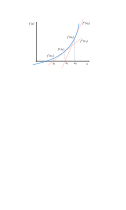
\includegraphics{figures/newton_method}
  \caption{Geometric interpretation of the Newton method in one dimension for an example function \(f\), whose derivative is denoted by \(f'\).}
  \label{fig:newton_method}
\end{figure}

In particular, using \(\pazocal R_\mathrm{J}\), a few simplifications can be obtained.
To ease the explanation, consider, a thermal residual operator $\pazocal{R}_{u}(\mathbf{u}, \bm{\uptheta})$ and a mechanical residual operator $\pazocal{R}_{\theta}(\mathbf{u}, \bm{\uptheta})$ defined to be the first and second components in the definition of \(\pazocal R_\mathrm{J}\) (Equation~\eqref{eq:def_res_gauss_seidel}).
Written in full
\begin{gather}
\pazocal{R}_{u}(\mathbf{u}, \bm{\uptheta})=\mathbf{u}-\pazocal{U}(\bm{\uptheta})=0, \\
\pazocal{R}_{\theta}(\mathbf{u}, \bm{\uptheta})=\bm{\uptheta}-\pazocal{T}(\mathbf{u})=0,
\end{gather}

From this, a block Newton iteration can be written as
\begin{highlight}
  \begin{equation} \label{eq:block_newton_raphson}
  \left[\begin{array}{l}
  J_{\pazocal{R}_{u}}\left(\mathbf u^k, \bm{\uptheta}^{k}\right) \\[7pt] J_{\pazocal{R}_{\theta}}\left(\mathbf{u}^{k}, \bm\uptheta^k\right)
  \end{array}\right]
  \left\{\begin{array}{c}\Delta \mathbf{u}^{k} \\ \Delta \bm{\uptheta}^{k}\end{array}\right\}
  =-\left\{\begin{array}{l}\pazocal{R}_{u}\left(\mathbf{u}^{k}, \boldsymbol{\theta}^{k}\right) \\ \pazocal{R}_{\theta}\left(\mathbf{u}^{k}, \boldsymbol{\theta}^{k}\right)\end{array}\right\},
  \end{equation}
\end{highlight}
and the update of the iteration variables reads
\begin{highlight}
  \begin{equation}
  \left\{\begin{array}{l}
  \mathbf{u}^{k+1} \\
  \boldsymbol{\theta}^{k+1}
  \end{array}\right\}=\left\{\begin{array}{l}
  \mathbf{u}^{k} \\
  \boldsymbol{\theta}^{k}
  \end{array}\right\}+\left\{\begin{array}{c}
  \Delta \mathbf{u}^{k} \\
  \Delta \boldsymbol{\theta}^{k}
  \end{array}\right\}.
  \end{equation}
\end{highlight}

The system of equations in Equation~\eqref{eq:block_newton_raphson} can be further simplified following \cite{degroote_development_2010} considering the definitions of the mechanical and thermal residuals and taking their derivatives.
It yields
\begin{equation}
\left[\begin{array}{cc}
\mathbf I & -J_{\pazocal{U}}\left(\bm{\uptheta}^{k}\right) \\[7pt]
-J_{\pazocal{T}}\left(\mathbf{u}^{k}\right) & \mathbf I
\end{array}\right]
\left\{\begin{array}{c}\Delta \mathbf{u}^{k} \\ \Delta \bm{\uptheta}^{k}\end{array}\right\}
=-\left\{\begin{array}{l}\pazocal{R}_{u}\left(\mathbf{u}^{k}, \boldsymbol{\theta}^{k}\right) \\ \pazocal{R}_{\theta}\left(\mathbf{u}^{k}, \boldsymbol{\theta}^{k}\right)\end{array}\right\},
\end{equation}

Solving for \(\Delta \mathbf u^k\) and \(\Delta \bm \uptheta^k\), one finds
\begin{align}
  \left(\mathbf I + J_\pazocal{U}(\bm\uptheta^k)J_\pazocal{T}(\mathbf u^k)\right)\Delta \mathbf u^k &= - \pazocal R_u(\mathbf u^k, \bm \uptheta^k)+J_\pazocal{U}(\bm\uptheta^k)\pazocal R_\theta(\mathbf u^k, \bm\uptheta^k), \label{eq:explicit_eq_delta_u_newton}\\
  \left(\mathbf I + J_\pazocal{T}(\mathbf u^k)J_\pazocal{U}(\bm\uptheta^k)\right)\Delta \bm\uptheta^k &= - \pazocal R_\theta(\bm \uptheta^k, \mathbf u^k)+J_\pazocal{\theta}(\mathbf u^k)\pazocal R_u(\mathbf u^k, \bm\uptheta^k). \label{eq:explicit_eq_delta_theta_newton}
\end{align}
Thus, the Jacobians now needed are \(J_\pazocal{U}\) and \(J_\pazocal{T}\).
See Section~\ref{sec:multisecant} for the practical application of this.

Every iteration of the Newton scheme involves at least one invocation of the thermal and mechanical solvers when computing $\pazocal{R}\left(\mathbf{u}^{k}\right)$ or both $\pazocal{R}_{u}\left(\mathbf{u}^{k}, \boldsymbol{\theta}^{k}\right)$ and $\pazocal{R}_{\theta}\left(\mathbf{u}^{k}, \boldsymbol{\theta}^{k}\right)$.
The critical point for black-box equation coupling is how to obtain the derivative information in the Jacobi matrices.
In different ways, some of the methods presented next find approximations for the required Jacobian times vector products.



\subsection{Constant Underrelaxation} \label{sec:underrelaxation}

One of the most straightforward ways to stabilize an iterative method is to use constant underrelaxation \citep{gatzhammer_efficient_2014}.
The relaxation is performed as follows
\begin{equation} \label{eq:constant_relaxation}
\mathbf x^{k+1}=(1-\omega) \mathbf x^{k}+\omega\left(\mathbf x^k - \pazocal R(\mathbf x^k)\right)=\mathbf x^{k} -\omega \pazocal R(\mathbf x^k),
\end{equation}
where \(\omega\) is the relaxation factor chosen in the range \(0<\omega<1\), which corresponds to an underrelaxation, to achieve a stabilizing effect.

Applying to Equation~\eqref{eq:def_res_jacobi}
\begin{equation}
  \left\{\begin{array}{c}
    \mathbf u^{k+1}\\
    \bm \uptheta^{k+1}
  \end{array}\right\} =
  (1-\omega)
  \left\{\begin{array}{c}
    \mathbf u^{k}\\
    \bm \uptheta^{k}
  \end{array}\right\}
  + \omega
  \left\{\begin{array}{c}
    \pazocal U(\bm\uptheta^k)\\
    \pazocal T(\mathbf u^k)
  \end{array}\right\}
\end{equation}
Applying to Equation~\eqref{eq:def_res_gauss_seidel}
\begin{equation}
  \bm\uptheta^{k+1} = (1-\omega)\bm\uptheta^k + \omega \pazocal T\circ\pazocal U(\bm \uptheta^k).
\end{equation}


Constant underrelaxation works well if \(\omega\) is close to 1 but leads to a slow convergence if \(\omega\) has to be chosen close to 0.
Thus, the constant underrelaxation method creates unmanageable computational costs for severe instabilities.
Overrelaxation can also be considered, keeping in mind that for \(\omega > 2\) convergence is lost.
The optimal \(\omega\) is not necessary the largest stable one \citep{gatzhammer_efficient_2014} and has to be set empirically.
In what follows, alternative methods are discussed to decrease the number of iterations necessary while maintaining stability.

\begin{framedbox}[htb]
  \caption{Constant underrelaxation applied to the block Gauss-Seidel scheme.}
  \label{box:constant_underrelaxation}
  \begin{center}
    \begin{minipage}{0.9\textwidth}
    \begin{enumerate}[(i)]
    \item \(\bm\uptheta^0 = \bm\uptheta_{n+1}^p\)
    \item Set fixed-point counter to zero: \(k=0\)
    \item Enter the fixed-point loop
    \begin{enumerate}[(1)]
      \item Solve the mechanical problem at fixed temeperature \(\bm \uptheta^k\): \(\mathbf u^{k+1} = \pazocal U(\bm \uptheta^k)\)
      \item Solve the thermal problem at a fixed configuration \(\mathbf u^{k+1}\): \(\bm \uptheta^{k+1} = \pazocal T(\mathbf u^{k+1})\)
      \item Compute \(\bm \uptheta^{k+1}\) using constant relaxation (Equation~\eqref{eq:constant_relaxation})
      \item If the desired accuracy has not been reached, update \(k=k+1\) and go to step (1).
    \end{enumerate}
    \end{enumerate}
    \end{minipage}
  \end{center}
\end{framedbox}

\section{One-point iteration function with memory}

\subsection{Aitken relaxation} \label{sec:aitken_relaxation}


The so-called Aitken \(\Delta^2\) relaxation method was introduced by \cite{irons_version_1969} as a modified Aitken \(\Delta^2\) that does not require the computation of the function twice per iteration as in the original method.
It has been widely used in the context of FSI \citep{irons_version_1969, kuttler_fixed-point_2008, joosten_analysis_2009, kuttler_vector_2009, erbts_partitioned_2015, wendt_partitioned_2015}.
It has also been used in the context of thermo-mechanics by \cite{danowski_monolithic_2013}.

In the one-dimensional case, this method resembles the secant method applied to the fixed point problem, which can be used to solve nonlinear equations without differentiation.
Calling it an Aitken method is perhaps a misnomer since, in the Aitken-Steffensen method, the function values are computed twice per iteration (see Section~\ref{sec:vector_extrapolation}).
It is more closely related to secant methods, reusing values from previous iterations.
This version of Aitken's \(\Delta^2\) method provides a dynamic under relaxation, which can be used to improve the convergence/stability properties of the coupling algorithm.

Assume that \(f\) is the function whose fixed point is sought.
The linear interpolation between two points already known of the function, \((a, f(a))\) and \((b, f(b)\) is
\begin{equation}
  y = \frac{f(b)-f(a)}{b-a}(x-a) + f(a).
\end{equation}
The fixed point of this approximation is
\begin{equation}
  c = \frac{f(b)-f(a)}{b-a}(c-a) + f(a).
\end{equation}
Thus, after rearranging,
\begin{equation}\
c=\frac{a f(b)- b f(a)}{\left(a-f(a)\right)-\left(b-f(b)\right)}
\end{equation}
This can be rewritten as
\begin{equation}
c=\left(1-\omega_{b}\right) b+\omega_{b} f(b) \quad \text { with } \omega_{b}=\frac{a-b}{\left(a-f(a)\right)-\left(b-f(b)\right)}
\end{equation}

Anticipating the next iteration step,
\begin{equation}
d=\left(1-\omega_{c}\right) c+\omega_{c} f(c) \quad \text { with } \omega_{c}=\frac{c-b}{\left(b-f(b)\right)-\left(c-f(c)\right)}
\end{equation}
a convenient expression for updating the relaxation factor may be found, i.e.
\begin{equation}
\omega_{c}=-\omega_{b}\frac{f(b)-b}{(c-f(c))-(f(b)-b)}.
\end{equation}
See Figure~\ref{fig:mod_aitken} for its geometric interpretation in one dimension.

\begin{figure}[htbp]
  \includegraphics{figures/mod_aitken}
  \caption{Geometric interpretation of the Aitken relaxation in one dimension for an example function \(f\) and corresponding interpreation as the secant method.}
  \label{fig:mod_aitken}
\end{figure}

Now, for the vector case, the next step is to work out the solution to the current iteration from the outcome of the previous iteration $\mathbf{x}^{k}$ plus a new increment $\Delta \mathbf{x}^{k}$
\begin{equation}
\mathbf{x}^{k+1}=\mathbf{x}^{k}+\Delta \mathbf{x}^{k}.
\end{equation}
The increment reads
\begin{equation} \label{eq:aitken_update}
\Delta \mathbf{x}^{k}=\omega^{k}\left(\pazocal S(\mathbf{x}^{(k)})-\mathbf{x}^{(k)}\right)=-\omega^{k} \pazocal R(\mathbf x^k).
\end{equation}
with $\omega^{k}$ being the relaxation coefficient.
This coefficient is updated in every iteration cycle as a function of two previous residuals
\begin{highlight}
  \begin{equation} \label{eq:aitken_relaxation_factor}
    \omega^{k}=-\omega^{k-1} \frac{\left(\mathbf{r}^{(k)}-\mathbf{r}^{(k-1)}\right)^{\mathrm{T}} \mathbf{r}^{(k-1)}}{\left(\mathbf{r}^{(k)}-\mathbf{r}^{(k-1)}\right)^{2}}.
  \end{equation}
\end{highlight}
Comparing with Equations~\eqref{eq:newton_system} and \eqref{eq:newton_iter}, \(\omega^{k}\) can be, in a sense, regarded as an approximation to the inverse of the Jacobian.
Dynamic relaxation is also easy to implement, and the additional computational input is acceptable since only inner vector products must be performed.
The dynamical relaxation coefficient is restricted to the range \((0,2)\) because employing relaxation with a relaxation coefficient outside this range leads to loss of convergence \citep{erbts_accelerated_2012}.
See Box~\ref{box:aitken_relaxation} for the pseudocode.

\begin{framedbox}[htb]
  \caption{Aitken relaxation for one timestep.}
  \label{box:aitken_relaxation}
  \begin{center}
    \begin{minipage}{0.9\textwidth}
    \begin{enumerate}[(i)]
    \item Set nonlinear counter to zero: \(k=0\)
    \item \(\mathbf x^k = \mathbf x_{n+1}^p\)
    \item Enter the nonlinear loop
    \begin{enumerate}[(1)]
      \item Compute \(\pazocal R(\mathbf x^k)\), which implies the solution of the mechanical and the thermal problems, \(\pazocal U\) and \(\pazocal T\), respectively.
      \item if \(k=0\):
      \begin{itemize}
        \item Compute \(\mathbf x^{k+1}\) using constant relaxation (Equation~\eqref{eq:constant_relaxation})
      \end{itemize}
      \item else:
      \begin{itemize}
        \item Compute \(\mathbf x^{k+1}\) using Aitken relaxation relaxation (Equations~\eqref{eq:aitken_update} and \eqref{eq:aitken_relaxation_factor})
        \item Save the current residue \(\mathbf r^k = \pazocal R^k\).
      \end{itemize}
      \item If the desired accuracy has not been reached, update \(k=k+1\) and go to step (1).
    \end{enumerate}
    \end{enumerate}
    \end{minipage}
  \end{center}
\end{framedbox}

\subsection{Multi-secant methods} \label{sec:multisecant}

The following exposition follows closely \cite{fang_two_2009}.
In quasi-Newton methods the Jacobian is updated in each iteration using a rank-one update.
Standard quasi-Newton methods require the updated \(J_{k+1}\) to satisfy the following secant condition
\begin{equation} \label{eq:secant_condition}
J_\pazocal{R}^{k+1} \Delta \mathbf x^{k}=\Delta \pazocal R^{k},
\end{equation}
where \(\Delta \pazocal R^{k}\equiv \pazocal R\left(\mathbf x^{k+1}\right)-\pazocal R\left(\mathbf x^ {k}\right)\).
Furthermore, another common requirement is the following so-called no-change condition
\begin{equation} \label{eq:no_change_condition}
J_\pazocal R^{k+1} \mathbf q=J_\pazocal R^{k} \mathbf q \quad \forall \mathbf q \text { such that } \mathbf q^{\mathrm{T}} \Delta \mathbf x^{k}=0,
\end{equation}
which stipulates that there be no new information from \(J_\pazocal R^{k}\) to \(J_\pazocal R^{k+1}\) along any direction \(\mathbf q\) orthogonal to \(\Delta \mathbf x^{k}\).

\cite{broyden_class_1965} developed a method satisfying both secant condition (Equation~\eqref{eq:secant_condition}) and the no-change condition (Equation~\eqref{eq:no_change_condition}), arriving at the update formula
\begin{highlight}
\begin{equation} \label{eq:good_update_broyden}
J_{\pazocal R}^{k+1}=J_{\pazocal R}^{k}+\left(\Delta \pazocal R^{k}-J_{\pazocal R}^{k} \Delta \mathbf x^{k}\right) \frac{\Delta {\mathbf x^{k}}^{\mathrm{T}}}{\Delta {\mathbf x^{k}}^{\mathrm{T}} \Delta \mathbf x^{k}}.
\end{equation}
\end{highlight}

Matrix \(J_\pazocal R^{k+1}\) in Equation~\eqref{eq:good_update_broyden} is the unique matrix satisfying both conditions \eqref{eq:secant_condition} and \eqref{eq:no_change_condition}.
The Broyden update can also be obtained by minimizing \(E\left(J_\pazocal R^{k+1}\right)=\left\|J_\pazocal R^{k+1}-J_\pazocal R^{k}\right\|_{F}^{2}\) with respect to terms of \(J_\pazocal R^{k+1}\), subject to the secant condition \eqref{eq:secant_condition}.

It may seem at first that Broyden's first method can be expensive since computing the quasi-Newton step \(\Delta \mathbf x^{k}\) requires solving a linear system at each iteration.
However, note that, typically, the approximate Jacobian is a small rank modification of a diagonal matrix (or a matrix that is easy to invert); hence, the cost to obtain this solution is not too high as long as the number of steps is not too large.

An alternative is Broyden's second method that approximates the inverse Jacobian instead of the Jacobian itself.
\(G_\pazocal R^{k}\) is used to denote the estimated inverse Jacobian at the \(k\) th iteration.
The secant condition (Equation~\eqref{eq:secant_condition}) now reads
\begin{equation} \label{eq:inverse_secant_cond}
G_\pazocal R^{k+1} \Delta \pazocal R^{k}=\Delta \mathbf x^{k}
\end{equation}
By minimizing \(E\left(G_\pazocal R^{k+1}\right)=\left\|G_\pazocal R^{k+1}-G_\pazocal R^{k}\right\|_{F}^{2}\) with respect to \(G_\pazocal R^{k+1}\) subject to Equation~\eqref{eq:inverse_secant_cond}, the following update formula is found for the inverse Jacobian
\begin{highlight}
  \begin{equation} \label{eq:bad_update_broyden}
  G_\pazocal R^{k+1}=G_\pazocal R^{k}+\left(\Delta \mathbf x_{k}-G_\pazocal R^{k} \Delta \pazocal R^{k}\right) \frac{\Delta {\pazocal R^{k}}^{\mathrm{T}}}{\Delta {\pazocal R^{k}}^{\mathrm{T}} \Delta \pazocal R^{k}}
  \end{equation}
\end{highlight}
which is also the only update satisfying both the secant condition (Equation~\eqref{eq:inverse_secant_cond}) and the no-change condition for the inverse Jacobian
\begin{equation}
  G_\pazocal R^{k} \mathbf q=G_\pazocal R^{k+1} \mathbf q \quad \forall \mathbf q \text { such that } \mathbf q^{\mathrm{T}} \Delta \pazocal R^{k}=0.
\end{equation}
The update formula in Equation~\eqref{eq:good_update_broyden} can also be obtained in terms of \(G_\pazocal R^{k} \equiv {J_\pazocal R^{k}}^{-1}\) by applying the Sherman-Morrison formula
\begin{equation} \label{eq:g_broyden_type_i}
G_\pazocal R^{k+1}=G_\pazocal R^{k}+\left(\Delta \mathbf x^{k}-G_\pazocal R^{k} \Delta \pazocal R^{k}\right) \frac{\Delta {\mathbf x^{k}}^{\mathrm{T}} G_\pazocal R^{k}}{\Delta {\mathbf x^{k}}^{\mathrm{T}} G_\pazocal R^{k} \Delta \pazocal R^{k}}
\end{equation}
This shows, as was explained earlier, that to solve the Jacobian system associated with Broyden's first approach can be reduced to a set of update operations that are not more costly than those required by the second update.
Note, however, that the above formula requires the inverse of the initial Jacobian.

From Equation~\eqref{eq:good_update_broyden} and Equation~\eqref{eq:bad_update_broyden} it is possible to define Broyden's family of updates, in which an update formula takes the general form
\begin{equation}
G_\pazocal R^{k+1}=G_\pazocal R^{k}+\left(\Delta \mathbf x^{k}-G_\pazocal R^{k} \Delta \pazocal R^{k}\right) \mathbf v_{k}^{\mathrm{T}}
\end{equation}
where \(\mathbf v_{k}^{\mathrm{T}} \Delta \pazocal R^{k}=1\) so that the secant condition \eqref{eq:secant_condition} holds.
Note that the secant condition \eqref{eq:inverse_secant_cond} is equivalent to condition \eqref{eq:secant_condition}.
% The pseudocode of Broyden's two methods is given in Box~\ref{box:broydens_method}.
Some authors called Broyden's first method Broyden's good update and Broyden's second method as Broyden's bad update.
These are two particular members of Broyden's family.

% \begin{framedbox}[htb]
%   \caption{Broyden's method for one timestep.}
%   \label{box:broydens_method}
%   \begin{center}
%     \begin{minipage}{0.9\textwidth}
%     \begin{enumerate}[(i)]
%     \item Set nonlinear counter to zero: \(k=0\)
%     \item \(\mathbf x^k = \mathbf x_{n+1}^p\)
%     \item Evaluate \(\pazocal R^k = \pazocal R(\mathbf x^k)\), which implies the solution of the mechanical and the thermal problems, \(\pazocal U\) and \(\pazocal T\), respectively.
%     \item Enter the nonlinear loop
%     \begin{enumerate}[(1)]
%       \item Compute the update step from \(\Delta \mathbf x^k = - G^k_\pazocal R \pazocal R^k\),
%       \item Update \(\mathbf x^{k+1} = \mathbf x^k + \Delta \mathbf x^k\),
%       \item Evaluate \(\pazocal R^{k+1} = \pazocal R(\mathbf x^{k+1})\), which implies the solution of the mechanical and the thermal problems, \(\pazocal U\) and \(\pazocal T\), respectively.
%       \item Compute \(\Delta \pazocal R^k = \pazocal R^{k+1} - \pazocal R^k\).
%       \item if the first update is to be used:
%       \begin{itemize}
%         \item Set \({{\mathbf{v}}^k}^T = \Delta {\mathbf x^k}^T G^k_\pazocal R\),
%       \end{itemize}
%       \item else if the second update is to be used:
%       \begin{itemize}
%         \item Set \({{\mathbf{v}}^k}^T = \Delta {\pazocal R^k}^T\),
%       \end{itemize}
%       \item \(G_\pazocal R^{k+1} = G_\pazocal R^k + (\Delta \mathbf x^k - G_\pazocal R^k\Delta \pazocal R^k)\frac{{{\mathbf{v}}^k}^T}{{{\mathbf{v}}^k}^T\Delta \pazocal R^k}.\)
%       \item If the desired accuracy has not been reached, update \(k=k+1\) and go to step (1).
%     \end{enumerate}
%     \end{enumerate}
%     \end{minipage}
%   \end{center}
% \end{framedbox}


\subsubsection{Generalized Broyden}

The multi-secant methods provide an approximation to the Jacobian in Equation~\eqref{eq:newton_system} or Equation~\eqref{eq:block_newton_raphson} using information from previous iterations.
A generalized Broyden's method with a flexible rank update on the inverse Jacobian, satisfying a set of \(m\) secant equations
\begin{equation} \label{eq:multi_secant_eqs}
  G_\pazocal R^{k} \Delta \pazocal R^{i}=\Delta \mathbf x^{i} \quad \text { for } i=k-m, \ldots, k-1
\end{equation}
where it is assumed \(\Delta \pazocal R^{k-m}, \ldots, \Delta \pazocal R^{k-1}\) are linearly independent and \(m \leqslant n\) can also be described.
Aggregating Equations~\eqref{eq:multi_secant_eqs} in matrix form, they can be rewriten it as
\begin{equation} \label{eq:multi_secant_eqs_mat}
  G_\pazocal R^{k} \mathscr{R}^{k}=\mathscr{X}^{k}.
\end{equation}
where
\begin{equation}
\mathscr{R}^{k}=\left[\Delta \pazocal R^{k-m} \cdots \Delta \pazocal R^{k-1}\right], \quad \mathscr{X}^{k}=\left[\Delta \mathbf x^{k-m} \cdots \Delta \mathbf x^{k-1}\right] \in \mathbb{R}^{n \times m}
\end{equation}
The no-change condition corresponding to \eqref{eq:no_change_condition} is
\begin{equation}
  \left(G_\pazocal R^{k}-G_\pazocal R^{k-m}\right) \mathbf q=0
\end{equation}
for all \(\mathbf q\) orthogonal to the subspace spanned by \(\Delta \pazocal R^{k-m}, \ldots, \Delta \pazocal R^{k-1}\), the columns of \(\mathscr{R}^{k}\).
In the end, this yields
\begin{equation}
  G_\pazocal R^{k}=G_\pazocal R^{k-m}+\left(\mathscr{X}^{k}-G_\pazocal R^{k-m} \mathscr{R}^{k}\right)\left({\mathscr{R}^{k}}^{\mathrm{T}} \mathscr{R}^{k}\right)^{-1} {\mathscr{R}^{k}}^{\mathrm{T}}
\end{equation}
a rank-\(m\) update formula.
Note that \(\operatorname{rank}\left(\mathscr{R}^{k}\right)=m\).
The update formula for \(\mathbf x^{k+1}\) is
\begin{align}
\mathbf x^{k+1} &=\mathbf x^{k}-G_\pazocal R^{k} \pazocal R^{k} \\
&=\mathbf x^{k}-G_\pazocal R^{k-m} \pazocal R^{k}-\left(\mathscr{X}^{k}-G_\pazocal R^{k-m} \mathscr{R}^{k}\right)\left({\mathscr{R}^{k}}^{\mathrm{T}} \mathscr{R}^{k}\right)^{-1} {\mathscr{R}^{k}}^{\mathrm{T}} \pazocal R^{k} \\
&=\mathbf x^{k}-G_\pazocal R^{k-m} \pazocal R^{k}-\left(\mathscr{X}^{k}-G_\pazocal R^{k-m} \mathscr{R}^{k}\right) \gamma_{k} \label{eq:update_gen_broyden_ls}
\end{align}
where the column vector \(\gamma_{k}\) is obtained by solving the normal equations \(\left({\mathscr{R}^{k}}^{\mathrm{T}} \mathscr{R}^{k}\right) \gamma_{k}={\mathscr{R}^{k}}^{\mathrm{T}} \pazocal R^{k}\), which is equivalent to solving the least squares problem
\begin{equation}
  \min _{\gamma}\left\|\mathscr{R}^{k} \gamma-\pazocal R^{k}\right\|_{2}.
\end{equation}
Note that in Equation~\eqref{eq:update_gen_broyden_ls}, if \(\mathscr{R}^{k}\) is square and of full rank, then for any \(G_\pazocal R^{k-m}\),
\begin{equation}
  \mathbf x^{k+1}=\mathbf x^{k}-\mathscr{X}^{k} {\mathscr{R}^{k}}^{-1} \pazocal R^{k},
\end{equation}
the same form as that in the standard secant method.

\subsubsection{Anderson mixing}

The Anderson mixing scheme [5] takes the latest \(m\) steps into account to obtain a better approximation to \(\mathbf x_{n+1}\) without evaluating \(\pazocal R\) again.
Consider
\begin{align}
  \bar{\mathbf x}^{k}=\mathbf x^{k}-\sum_{i=k-m}^{k-1} \gamma_{i}^{k} \Delta \mathbf x^{i}=\mathbf x_{k}-\mathscr{X}^{k} \gamma^{k}, \label{eq:anderson_x_bar}\\
  \bar{\pazocal R}^{k}=\pazocal R^{k}-\sum_{i=k-m}^{k-1} \gamma_{i}^{k} \Delta \pazocal R^{i}=\pazocal R^{k}-\mathscr{R}^{k} \gamma^{k} \label{eq:anderson_r_bar},
\end{align}
where \(\Delta \mathbf x^{i}=\mathbf x^{i+1}-\mathbf x^{i}\) and \(\Delta \pazocal R^{i}=\pazocal R^{i+1}-\pazocal R^{i}\), \(\mathscr{X}^{k}=\left[\Delta \mathbf x^{k-m} \cdots \Delta \mathbf x^{k-1}\right]\), \(\mathscr{R}^{k}=\left[\Delta \pazocal R^{k-m} \cdots \Delta \pazocal R^{k-1}\right]\), and \(\gamma^{k}=\left[\gamma_{k-m}^{k} \cdots \gamma_{k-1}^{k}\right]^{\mathrm{T}}\).
Expressing the equations in the form \(\bar{\mathbf x}^{k}=\sum_{j=k-m}^{k} w_{j} \mathbf x^{j}\) and \(\bar{\pazocal R}^{k}=\sum_{j=k-m}^{k} w_{j} \pazocal R^{j}\), it is found that \(\sum_{j=k-m}^{k} w_{j}=1\).
In other words, \(\bar{\mathbf x}_{k}\) and \(\bar{\pazocal R}_{k}\) are weighted averages of \(\mathbf x_{k-m}, \ldots, \mathbf x_{k}\) and \(\pazocal R^{k-m}, \ldots, \pazocal R^{k}\), respectively.
The arguments \(\gamma^{k}=\left[\gamma_{k-m}^{k} \cdots \gamma_{k-1}^{k}\right]^{\mathrm{T}}\) are determined by minimizing
\begin{equation}
E\left(\gamma^{k}\right)=\left\langle\bar{\pazocal R}^{k}, \bar{\pazocal R}^{k}\right\rangle=\left\|\pazocal R^{k}-\mathscr{R}^{k} \gamma^{k}\right\|_{2}^{2}
\end{equation}
whose solution can, but should not in practice, be obtained by solving the normal equations
\begin{equation}
\left({\mathscr{R}^{k}}^{\mathrm{T}} \mathscr{R}^{k}\right) \gamma^{k}={\mathscr{R}^{k}}^{\mathrm{T}} \pazocal R^{k}. \label{eq:normal_eqs_anderson}
\end{equation}
Combining Equations~\eqref{eq:anderson_x_bar}, \eqref{eq:anderson_r_bar}, and \eqref{eq:normal_eqs_anderson}, one obtains
\begin{align}
\mathbf x^{k+1} &=\bar{\mathbf x}^{k}+\beta \bar{\pazocal R}^{k} \\
&=\mathbf x^{k}+\beta \pazocal R^{k}-\left(\mathscr{X}^{k}+\beta \mathscr{R}^{k}\right) \gamma^{k} \\
&=\mathbf x^{k}+\beta \pazocal R^{k}-\left(\mathscr{X}^{k}+\beta \mathscr{R}^{k}\right)\left({\mathscr{R}^{k}}^{\mathrm{T}} \mathscr{R}^{k}\right)^{-1} {\mathscr{R}^{k}}^{\mathrm{T}} \pazocal R^{k} \label{eq:update_anderson_mixing}
\end{align}
where \(\beta\) is the preset mixing parameter and \({\mathscr{R}^{k}}^{\mathrm{T}} \mathscr{R}^{k}\) is assumed to be nonsingular.
In particular, if no previous iterate is taken into account (i.e. \(m=0\) ), then Equation~\eqref{eq:update_anderson_mixing} reads
\begin{equation}
  \mathbf x^{k+1}=\mathbf x^{k}+\beta \pazocal R^{k}
\end{equation}
This scheme is referred to as simple mixing and underrelaxation if \(0<\beta<1\) (see Section~\ref{sec:underrelaxation}).
The update formula \eqref{eq:update_anderson_mixing} is the same as \eqref{eq:update_gen_broyden_ls} by setting \(G_\pazocal R^{k-m}=-\beta \mathbf I\).
In this respect Anderson mixing implicitly forms an approximate inverse Jacobian \(G_\pazocal R^{k}\) that minimizes \(\left\|G_\pazocal R^{k}+\beta \mathbf I\right\|_{F}\) subject to \eqref{eq:multi_secant_eqs_mat}.
In the context of mixing, generalized Broyden's second method is equivalent to Anderson mixing.
Note that if \(\mathscr{R}^{k}\) is square and nonsingular, then Equation~\eqref{eq:update_anderson_mixing} matches the formula of the standard secant method.

\subsubsection{Generalized Broyden's family} \label{sec:gen_broyden_fam}

Now we can write down the generalized Broyden family, in which an update algorithm is in the form
\begin{equation} \label{eq:inv_jacob_gen_broyden}
G_\pazocal R^{k}=G_\pazocal R^{k-m}+\left(\mathscr{X}^{k}-G_\pazocal R^{k-m} \mathscr{R}^{k}\right) {V^{k}}^{\mathrm{T}}
\end{equation}
where \({V^{k}}^{\mathrm{T}} \mathscr{R}^{k}=I\) so that the secant condition \(G_\pazocal R^{k} \mathscr{R}^{k}=\mathscr{X}^{k}\) holds.
The two optimal choices of \({V^k}^T = {M^k}^{-1}{N^k}^T\) are
\begin{equation} \label{eq:broyden_type_ii}
  {M^k} = {\mathscr R^k}^T \mathscr R^k,\quad {N^k}^T = {\mathscr R^k}^T,
\end{equation}
minimizaing \(\left\|G_\pazocal R^k - G_\pazocal R^{k-m}\right\|_F\) and
\begin{equation} \label{eq:broyden_type_i}
  {M^k} = {\mathscr X^k}^T G_\pazocal R^k \mathscr R^k,\quad {N^k}^T = {\mathscr X^k}^T G_\pazocal R^k,
\end{equation}
minimizaing \(\left\|J_\pazocal R^k - J_\pazocal R^{k-m}\right\|_F\).
This last choice yields as the approximation for the Jacobian
\begin{equation}
  J_\pazocal R^{k}=J_\pazocal R^{k-m}+\left(\mathscr{R}^{k}-J_\pazocal R^{k-m} \mathscr{X}^{k}\right)\left({\mathscr{X}^{k}}^{\mathrm{T}} \mathscr{X}^{k}\right)^{-1} {\mathscr{X}^{k}}^{\mathrm{T}},
\end{equation}
after applying the Woodbury formula.
The first choice is said to correspond to a Type-II update and the second to a Type-I update \citep{fang_two_2009}.

% \begin{framedbox}[htb]
%   \caption{Generalized Broyden's family method for one timestep.}
%   \label{box:broydens_method}
%   \begin{center}
%     \begin{minipage}{0.9\textwidth}
%     \begin{enumerate}[(i)]
%     \item Set nonlinear counter to zero: \(k=0\)
%     \item Set \(\mathbf x^k = \mathbf x_{n+ 1}^p\) and choose an initial estimate for \(\mathbf G_1 = J^{-1}_\pazocal R(\mathbf x^k)\).
%     \item Evaluate \(\pazocal R^k = \pazocal R(\mathbf x^k)\), which implies the solution of the mechanical and the thermal problems, \(\pazocal U\) and \(\pazocal T\), respectively.
%     \item Enter the nonlinear loop
%     \begin{enumerate}[(1)]
%       \item Compute the update step from \(\Delta \mathbf x^k = - G^k_\pazocal R \pazocal R^k\) and add it to \(\mathscr X^k\). If the maximum number of previous iteration \(m\) replace the oldest column.
%       \item Update \(\mathbf x^{k+1} = \mathbf x^k + \Delta \mathbf x^k\),
%       \item Evaluate \(\pazocal R^{k+1} = \pazocal R(\mathbf x^{k+1})\), which implies the solution of the mechanical and the thermal problems, \(\pazocal U\) and \(\pazocal T\), respectively.
%       \item Compute \(\Delta \pazocal R^k = \pazocal R^{k+1} - \pazocal R^k\) and add it to \(\mathscr R^k\). If the maximum number of previous iteration has been reach replace the oldest column.
%       \item Compute \({\mathbf V^k}^T\) according to the type of update chosen (Equation~\eqref{eq:broyden_type_i} and \eqref{eq:broyden_type_ii}).
%       \item \(G_\pazocal R^{k+1} = G_\pazocal R^k + (\mathscr X^k - G_\pazocal R^k\mathscr R^k){{\mathbf{V}}^k}^T.\)
%       \item If the desired accuracy has not been reached, update \(k=k+1\) and go to step (1).
%     \end{enumerate}
%     \end{enumerate}
%     \end{minipage}
%   \end{center}
% \end{framedbox}

\subsubsection{Anderson's family}

The udpate formula for Anderson's family can be found from Equation~\eqref{eq:inv_jacob_gen_broyden} using as the approximation to the previous Jacobian the identity matrix multiplied by a constant \(\beta\), i.e.,
\begin{equation} \label{eq:andersons_family_update}
  \mathbf x^{k+1} = \mathbf x^{k} + \beta \pazocal R^k - (\mathscr X^k + \beta\mathscr R^k){\mathbf V^k}^T \pazocal R^k.
\end{equation}
The two choices for \(\mathbf V^k\) remain the same, replacing \(G_\pazocal R^{k-m}\) by \(-\beta\mathbf I\).
They now minimize \(\|G_\pazocal R^k+\beta\mathbf I\|\) and \(\|J_\pazocal R^k + (1/\beta)\mathbf I\|\).

% \begin{framedbox}[htb]
%   \caption{Anderson's family method for one timestep.}
%   \label{box:broydens_method}
%   \begin{center}
%     \begin{minipage}{0.9\textwidth}
%     \begin{enumerate}[(i)]
%     \item Set \(\mathbf x^0 = \mathbf x_{n+ 1}^p\).
%     \item Evaluate \(\pazocal R^0 = \pazocal R(\mathbf x^k)\), which implies the solution of the mechanical and the thermal problems, \(\pazocal U\) and \(\pazocal T\), respectively.
%     \item Compute \(\mathbf x^1 = \mathbf x^0 + \beta R^0\).
%     \item Evaluate \(\pazocal R^{1} = \pazocal R(\mathbf x^{1})\), which implies the solution of the mechanical and the thermal problems, \(\pazocal U\) and \(\pazocal T\), respectively.
%     \item Set nonlinear counter to zero: \(k=1\)
%     \item Enter the nonlinear loop
%     \begin{enumerate}[(1)]
%       \item Compute \(\Delta \pazocal R^{k-1} = \pazocal R^{k} - \pazocal R^{k-1}\) and add it to \(\mathscr R^k\).
%       If the maximum number of previous iteration has been reached either replace the oldest column or restart \(\mathscr R^k\).
%       \item Compute \(\Delta \mathbf x^{k-1} = \mathbf x^{k} -\mathbf x^{k-1} \) and add it to \(\mathscr X^k\).
%         If the maximum number of previous iteration has been reached either replace the oldest column or restart \(\mathscr X^k\).
%       \item Compute \({\mathbf V^k}^T\) according to the type of update chosen (Equation~\eqref{eq:broyden_type_i} and \eqref{eq:broyden_type_ii}).
%       \item Update according to \(\mathbf x^{k+1} = \mathbf x^k + \beta \pazocal R^k + \left(\mathscr X^k + \beta\mathscr R^k\right){\mathbf V^k}^T\pazocal R^k \).
%       \item Evaluate \(\pazocal R^{k+1} = \pazocal R(\mathbf x^{k+1})\), which implies the solution of the mechanical and the thermal problems, \(\pazocal U\) and \(\pazocal T\), respectively.
%       \item If the desired accuracy has not been reached, update \(k=k+1\) and go to step (1).
%     \end{enumerate}
%     \end{enumerate}
%     \end{minipage}
%   \end{center}
% \end{framedbox}

\subsubsection{The Broyden-like class}

Both the generalized Broyden's family and Anderson's family can be understood as methods in the Broyden-like class as described in \cite{fang_two_2009}.
Ssuppose the latest \(m\) iterates are available, which are denoted by \(\mathbf x^{1}, \ldots, \mathbf x^{m}\).
Let \(\Delta \mathbf x^{i}=\mathbf x^{i+1}- \mathbf x^{i}\) for \(i=1, \ldots, m-1\).
Partition \(\Delta \mathbf x^{1}, \ldots, \Delta \mathbf x^{m-1}\) into \(p\) groups,
\begin{align}
\mathscr{X}^{1} & =\left[\Delta \mathbf x^{1}, \ldots, \Delta \mathbf x^{z_{1}}\right], \\
\mathscr{X}^{2} & =\left[\Delta \mathbf x^{z_{1}+1}, \ldots, \Delta \mathbf x^{z_{2}}\right],\\
& \vdots \\
\mathscr{X}^{p} & =\left[\Delta \mathbf x^{z_{k-1}+1}, \ldots, \Delta \mathbf x^{z_{k}}\right],
\end{align}
where \(z_{i}\) is the index of the last entry in the \(i\) th group for \(i=1, \ldots, p\); \(z_{0}=0\) and \(z_{p}=m-1\).
Also partition \(\Delta \pazocal R^{1}, \ldots, \Delta \pazocal R^{m-1}\) into \(\mathscr R^{1}, \ldots, \mathscr R^p\) accordingly, where \(\Delta \pazocal R^{i}=\pazocal R^{i+1}- \pazocal R^{i}\) with \(\pazocal R^{i}=\pazocal R(\mathbf x^{i})\).  The sizes of the groups for \(i=1, \ldots, k\) are denote by \(s_{i}:=z_{i}-z_{i-1}\).
Note that the indexing here is different from the previous sections.
The inverse of the Jacobian is iteratively approximated at the \(\left(z_{i}+1\right)\)st iterate for \(i=1, \ldots, p\) as
\begin{equation} \label{sec:broyden_like_class_g_update}
  G_\pazocal R^{i+1} = G_\pazocal R^{i}+\left(\mathscr{X}^{i}-G_\pazocal R^{i} \mathscr R^{i}\right) {\mathbf V^{i}}^T,
\end{equation}
where \({\mathbf V^{i}}^T \mathscr{R}^{i}=\mathbf I\) for the secant condition.
The update follows the formula of the generalized Broyden family.
In the context of mixing, the base case is
\begin{equation}
  G_\pazocal R^{1}=-\beta \mathbf I,
\end{equation}
where \(\beta\) is the mixing parameter.
The next iterate is set as
\begin{equation} \label{eq:update_broyden_family}
  \mathbf x^{m+1}=\mathbf x^{m}-G_\pazocal R^{k+1} \pazocal R^m.
\end{equation}
The choice of \(V_{i}\) satisfying \(V_{i}^{\mathrm{T}} \mathscr{F}_{i}=I\) is performed as described in Section~\ref{sec:gen_broyden_fam}.

\subsection{Practical considerations}

The application of Broyden's method as described so far is unfeasible for the problems considered in this document, i.e., thermo-mechanical coupled problems with many unknowns.
So far, the descriptions considered of the Broyden-like class methods require one to keep the large \(G_\pazocal R^i\) matrices of size \(n_\text{unknowns}\times n_\text{unknowns}\) in memory, in addition to the previous iterates.
This is a significant drawback.
However, \cite{fang_two_2009} present a more memory efficient way of implementing these methods.
Let
\begin{equation} \label{eq:def_e_broyden}
E^{i}=\mathscr{X}^{i}-G_\pazocal R^{i} \mathscr R^{i}.
\end{equation}
Substituting Equation~\eqref{eq:def_e_broyden} into Equation~\eqref{sec:broyden_like_class_g_update} one obtains
\begin{align}
  G_\pazocal R^{i}=& G_\pazocal R^{i-1}+E^{i-1} {V^{i-1}}^T, \\
  =& G_\pazocal R^{i-2} + E^{i-2} {V^{i-2}}^T + E^{i-1} {V^{i-1}}^T, \\
  & \vdots \\
  =& G_\pazocal R^{1}+\sum_{j=1}^{i-1} E^{j} {V^{j}}^{\mathrm{T}}, \label{eq:update_broyden_family_g_mem}
\end{align}
for \(i=2, \ldots, p+1\).
Matrices \(G_\pazocal R^{i}\) need not be explicitly stored.
\(G_\pazocal R^{i}\) is needed  only to compute \(G_\pazocal R^{i} \mathscr R^{i}\) in Equation~\eqref{eq:def_e_broyden} and \(G_\pazocal R^{p+1} \pazocal R^{m}\) in Equation~\eqref{eq:update_broyden_family}, and also for \(V^{i}\) if it depends on \(G_\pazocal R^{i}\).
Substituting Equation~\eqref{eq:update_broyden_family_g_mem} into Equation~\eqref{eq:def_e_broyden} obtains
\begin{equation} \label{eq:update_eq_for_e}
E^{i}=\mathscr{X}^{i}-G_\pazocal R^1 \mathscr{R}^{i}-\sum_{j=1}^{i-1} E^{j}\left({V^{j}}^T \mathscr{R}^{i}\right),
\end{equation}
for \(i=1, \ldots, p\).
The computation is economic for large-scale problems with \(n \gg m\).
The next iterate \(\mathbf x^{m+1}\) in (32) can also be computed in a similar manner
\begin{equation} \label{eq:mem_eff_update_broyden}
  \mathbf x^{m+1}=\mathbf x^{m} - G_\pazocal R^{p+1} \pazocal R^{m}= \mathbf x^{m} - G_\pazocal R^1 \pazocal R^{m}-\sum_{j=1}^{k} E^{j}\left({V^{j}}^T \pazocal R^m\right).
\end{equation}

Using Type-II update, the computation of \(V^{i}\) is straightforward from \(\mathscr{R}^{i}\).
On the other hand, Type-I update involves \(G_\pazocal R^{i}\) to compute \(V^{i}\).
Thus
\begin{equation} \label{eq:compute_n_broyden}
  {N^{i}}^T={\mathscr{X}^{i}}^T G_\pazocal R^{i}=G_\pazocal R^1 {\mathscr{X}^{i}}^T+\sum_{j=1}^{i-1}\left({\mathscr{X}^{i}}^{\mathrm{T}} E^{j}\right) {V^{j}}^T.
\end{equation}
After obtaining \(N^{i}\), we compute \(M^{i}={N^{i}}^T \mathscr{R}^{i}\) and then \({V^{i}}^T={M^{i}}^{-1} {N^{i}}^T\) for \(i=1, \ldots, p\).

Looking at Equations~\eqref{eq:update_eq_for_e}, \eqref{eq:mem_eff_update_broyden} and \eqref{eq:compute_n_broyden}, one still needs the initial approximation to the inverse of the Jacobian, \(G_\pazocal R^1\), whose size is \(n_\text{unknown}\times n_\text{unknown}\).
In \cite{fang_two_2009} the approach adopted was to follow the idea of Anderson's mixing and set
\begin{equation}
  G_\pazocal R^1 = - \beta \mathbf I,
\end{equation}
drastically improving the memory requirements, as only one scalar parameter, \(\beta\), needs to be saved.
Also, \cite{kelley_solving_2003}, assumes in his implementation of Broyden's method, an initial approximation to \(G_\pazocal R^1\) equal to the identity matrix.
Information about \(G_\pazocal R^1\) is applied in the preconditioning of the system instead.

To compute \(V^i\), \cite{fang_two_2009} suggest a \(QR\) decomposition with pivoting.
Be it for a Type-II update, where one needs to solve a least-squares problem, or for a Type-I update, one needs to invert a generally non-symmetric matrix.
This approach leads to better numerical stability when the matrices to be inverted are singular or ill-conditioned, compared with solving the normal equations.
The \(QR\) decomposition has a computational cost of \(\pazocal O(n_\text{unknown}m^2)\) algebraic operations \citep{dennis_numerical_1996}.

If the size of the groups \(s_1, s_2,\dots\) are fixed from one Newton iteration to the next, so the \(E^i\) and \(V^i\) matrices remain the same from one iteration to the next, the computation effort to compute them is saved from one iteration to the next.
Here only constant \(s=s_1=s_2 =\cdots\) is considered, where \(s=\infty\) corresponds to Anderson's mixing, where all previous iterates available are considered.

One question remains. How to proceed when the available memory runs out?.
According to \cite{kelley_solving_2003}, as is often the case with GMRES, the iteration can be restarted if there is no more room to store the vectors.
A different approach, called limited memory in the optimization literature, is to replace the oldest of the stored steps with the most recent one.

Thus, appplying the method as suggest by \cite{fang_two_2009}, leads to a storage need of
\begin{enumerate}
  \item  Two column vectors of size \(n_\text{unknown}\) for \(\mathbf x^{m}\) and \(\pazocal R^{m}\).
  \item An \(n_\text{unknown} \times(m-1)\) matrix for \(\mathscr{X}^{1}, \ldots, \mathscr{X}^{k}\) (shared with \(E^{1}, \ldots, E^{k}\)).
  \item An \(n_\text{unknown} \times(m-1)\) matrix for \(\mathscr{R}^{1}, \ldots, \mathscr{R}^{k}\) (shared with \(V^{1}, \ldots, V^{k}\) ).
  \item For Type-I update we also store the last group \(N^{k}\), since its computation involves \(G_\pazocal R^{k}\).
\end{enumerate}
and for each nonlinear iteration the computational cost is \(\pazocal O(n_\text{unknown}m^2)\).
For \(m=1\), \(V^i\) can be directly computed without needing to invert matrices, and the cost comes down to \(\pazocal O(n_\text{unknown})\) per nonlinear iteration.
Also, when \(k\) is different from any \(z_i\) a group is being complete, one can either use a shortened group or reuse the approximation to the Jacobian without using the new information.
This save computational effort and those iteration cost only \(\pazocal O(n_\text{unknown})\).
See in Box~\ref{box:broydens_family} the pseudocode for the Broyden-like family with restart.

\begin{framedbox}[htb]
  \caption{Broyden-like class methods for one timestep with restart.}
  \label{box:broydens_family}
  \begin{center}
     \begin{minipage}{0.9\textwidth}
     \begin{enumerate}[(i)]
     \item Set \(\mathbf x^1 = \mathbf x_{n+ 1}^p\).
     \item Evaluate \(\pazocal R^1 = \pazocal R(\mathbf x^1)\), which implies the solution of the mechanical and the thermal problems, \(\pazocal U\) and \(\pazocal T\), respectively.
     \item Compute \(\mathbf x^2 = \mathbf x^1 + \beta R^1\).
     \item Evaluate \(\pazocal R^{2} = \pazocal R(\mathbf x^{2})\), which implies the solution of the mechanical and the thermal problems, \(\pazocal U\) and \(\pazocal T\), respectively.
     \item Intialize counters: \(k=2\) and \(i=1\)
     \item Enter the nonlinear loop
     \begin{enumerate}[(1)]
       \item If the maximum number of previous iteration \(m\) has been reached restart all \(\mathscr X^i\) and \(\mathscr R^i\) and set \(i=1\).
       \item Compute \(\Delta \pazocal R^{k-1} = \pazocal R^{k} - \pazocal R^{k-1}\) and add it to \(\mathscr R^i\).
       \item Compute \(\Delta \mathbf x^{k-1} = \mathbf x^{k} -\mathbf x^{k-1} \) and add it to \(\mathscr X^i\).
      \item If \(s=\infty\) (Anderson mixng):
      \begin{itemize}
        \item Compute \({V^i}^T\) according to the type of update chosen (Equation~\eqref{eq:broyden_type_i} and \eqref{eq:broyden_type_ii}).
        \item Update according to \(\mathbf x^{k+1} = \mathbf x^k + \beta \pazocal R^k - (\mathscr X^i + \beta\mathscr R^i){V^i}^T\pazocal R^k\).
      \end{itemize}
      \item else:
      \begin{itemize}
        \item If \(k= z_j + 1\) for any \(j\geq 1\), compute \(E^i\) (Equation~\eqref{eq:update_eq_for_e}) and \({ V^i}^T\) according to the type of update chosen (Equation~\eqref{eq:broyden_type_i} and \eqref{eq:broyden_type_ii}). Save them on \(\mathscr X^i\) and \(\mathscr R^i\), respectively. Update \(i=i+1\).
        \item Update according to \(\mathbf x^{k+1} = \mathbf x^k + \beta \pazocal R^k - \sum_{j=1}^{i-1} E^j ({V^j}^T\pazocal R^k)\).
      \end{itemize}
       \item Evaluate \(\pazocal R^{k+1} = \pazocal R(\mathbf x^{k+1})\), which implies the solution of the mechanical and the thermal problems, \(\pazocal U\) and \(\pazocal T\), respectively.
       \item If the desired accuracy has not been reached, update \(k=k+1\) and go to step (1).
     \end{enumerate}
     \end{enumerate}
     \end{minipage}
   \end{center}
\end{framedbox}

\cite{kelley_solving_2003} presents for the Broyden method an implementation that halves the memory requirement relative to the one present in \cite{fang_two_2009}.
It is based on the Type-I update and to deduce it consider Equation~\eqref{eq:good_update_broyden} and Sherman-Morrison formula
\begin{equation}
  \left(J_\pazocal R+ \mathbf u \mathbf v^{T}\right)^{-1}=\left(\mathbf I- \frac{\left(G_\pazocal R \mathbf u\right) \mathbf v^{T}}{1+\mathbf v^{T} G_\pazocal R \mathbf u}\right) G_\pazocal R,
\end{equation}
where as before \(G_\pazocal R\equiv J_\pazocal R^{-1}\).
One can rewrite Equation~\eqref{eq:good_update_broyden} as
\begin{equation}
  J_\pazocal R^{k+1}=J_\pazocal R^k+ \mathbf u^k {\mathbf v^k}^{T},
\end{equation}
where
\begin{equation}
  \mathbf u^k=\left(\Delta \pazocal R^k - J_\pazocal R^k \Delta \mathbf x^{k}\right) /\left\|\Delta \mathbf x^{k}\right\| \text { and } \mathbf v^{k}=\Delta \mathbf x^{k} /\left\|\Delta \mathbf x^{k}\right\|.
\end{equation}
Then, keeping in mind that \(J_\pazocal R^{1}=\mathbf I\),
\begin{align}
G_\pazocal R^{k+1} &=\left(\mathbf I - \mathbf w^{k} {\mathbf v^{k}}^{T}\right)\left(\mathbf I - \mathbf w_{k-1} {\mathbf v^{k-1}}^{T}\right) \cdots\left(\mathbf I-\mathbf w^{1} {\mathbf v^{1}}^{T}\right) G_\pazocal R^1, \\
&=\prod_{j=0}^{k}\left(\mathbf I-\mathbf w^{j} {\mathbf v^{j}}^{T}\right),
\end{align}
where, for \(k \geq 0\),
\begin{equation}
  \mathbf w^{k}=\displaystyle\frac{G_\pazocal R^k \mathbf u^{k}}{1 + {\mathbf v^{k}}^{T} G_\pazocal R^k \mathbf u^{k}}.
\end{equation}
So, to apply \(G_\pazocal R^{k+1}\) to a vector \(\mathbf p\), the is cost of \(O(n_\text{unknown} k)\) floating point operations and storage of the \(2 k\) vectors \(\left\{\mathbf w^{j}\right\}_{j=1}^{k}\) and \(\left\{\Delta \mathbf x^{j}\right\}_{j=1}^{k}\).
The storage can be halved with a trick (see \cite{kelley_solving_2003} for details)
\begin{align}
\Delta \mathbf x^{k} &= - G_\pazocal R^{k+1}  \pazocal R^k,\\
&=-\left(\mathbf I-\frac{\mathbf w^{k} {\Delta \mathbf x^{k}}^{T}}{\left\|\Delta \mathbf x^{k}\right\|}\right) G_\pazocal R^k \pazocal R^k, \\
&= - \frac{G_\pazocal R^k R^k}{1 + {\Delta \mathbf x^k}^T G_\pazocal R^k \pazocal R^k /\|\Delta \mathbf x^k\|^2}.
\end{align}

According to \cite{kelley_solving_2003}, the Sherman-Morrison approach is more efficient, in terms of both time and storage, than dense matrix approaches proposed elsewhere.
For example, the approach presented in \cite{dennis_numerical_1996} has a \(\pazocal O(n_\text{unknown})\) cost per nonlinear iteration and requires one to keep in memory the \(QR\) decomposition of the previous approximation to the Jacobian.
However, the dense matrix approach can detect ill-conditioning in the approximate Jacobians.
Bounded deterioration implies that the Broyden matrices will be well-conditioned if the data is sufficiently good, and superlinear convergence suggests that only a few iterates will be needed.


\paragraph{In the context of FSI}

The multi-secant quasi-Newton methods have been used in the context of FSI, although not always presented as such \citep{haelterman_quasi-newton_2009, gatzhammer_efficient_2014, uekermann_partitioned_2016, scheufele_coupling_2018}.
 \cite{vierendeels_implicit_2007} and \cite{degroote_stability_2008} consider the system of equations \eqref{eq:explicit_eq_delta_u_newton} and \eqref{eq:explicit_eq_delta_theta_newton}, where recall that an estimate for the Jacobians \(J_\pazocal{U}\) and \(J_\pazocal{T}\) is needed.
The authors achieve this by using linear reduced-order models for the fluid solver and the structure solver.
These are set up from solver input and output deltas or sensitivities during the coupling iterations.
The resulting method for two black-box solvers is called interface block quasi-Newton method with least-squares approximation (IBQN-LS) in \cite{degroote_development_2010}.

This approach can be understood in the framework of the multi-secant quasi-Newton methods presented above and originating in \cite{fang_two_2009} as follows.
If one looks at \(\beta\mathbf I - (\mathscr X^k + \beta\mathscr R^k){\mathbf V^k}^T\) in Equation~\eqref{eq:andersons_family_update} as, in a sense, an approximation to the inverse of the Jacobian (compare with Equation~\eqref{eq:inv_jacob_gen_broyden}).
The corresponding Jacobian is given by
\begin{equation}
  J_\pazocal R^k = \alpha\mathbf I + (\mathscr R^k - \alpha\mathbf I\mathscr X^k )({\mathscr X^k}^T\mathscr X^k)^{-1}{\mathscr X^k}^T,
\end{equation}
where \(\alpha=1/\beta\).
If one sets \(\alpha=0\), the approximation to the Jacobian obtained is
\begin{equation}
  J_\pazocal R^k = \mathscr R^k({\mathscr X^k}^T\mathscr X^k)^{-1}{\mathscr X^k}^T.
\end{equation}
This corresponds to the linear reduced order models in \cite{vierendeels_implicit_2007}, where \(\pazocal R\) is replaced by the functions corresponding to the fluid and structure solvers.
If the functions considered are instead the mechanical and thermal solvers, this method can easily be applied to the thermomechanical problem.
The block \(({\mathscr X^k}^T\mathscr X^k)^{-1}{\mathscr X^k}^T\) can be understood as being a part of a least-squares solution, the so-called normal equations, i.e., the equations whose solution also solve the minimization problem
\begin{equation}
  \arg\min_{\tilde{\gamma}} \|\Delta \mathbf x - \mathscr{X}^k\tilde{\gamma}\|_2.
\end{equation}
As such one can avoid the use of the normal equations and employ more numerically stable and efficient methods such economy size \(QR\)-decomposition.
In addition, \cite{vierendeels_implicit_2007} solve the system of equation \eqref{eq:explicit_eq_delta_u_newton} and \eqref{eq:explicit_eq_delta_theta_newton} in a Gauss-Seidel manner, using always the most recent values available to estimate the Jacobians.

An interface quasi-Newton method based on Equation~\eqref{eq:newton_system} and Equation~\eqref{eq:newton_iter} is presented in \cite{degroote_development_2010} for FSI.
The method is called interface quasi-Newton with an approximation of the inverse of the interface Jacobian matrix by least squares (QIN-ILS).
Its origin is the IBQN-LS method presented in \cite{vierendeels_implicit_2007}, and it employs only one reduced-order model for the inverse of the overall interface Jacobian matrix of the Newton system (Equation~\eqref{eq:newton_system}) applied to the right-hand side vector.

If in Equation~\eqref{eq:update_anderson_mixing}, corresponding to Anderson's mixing, one sets \(\beta=-1\), the update formula comes out to be
\begin{equation}
  \mathbf x^{k+1} = \mathbf x^k - \pazocal R^k - (\mathscr X^k - \mathscr R^k)\left({\mathscr{R}^{k}}^{\mathrm{T}} \mathscr{R}^{k}\right)^{-1} {\mathscr{R}^{k}}^{\mathrm{T}} \pazocal R^{k}.
\end{equation}
Using the definition for the fixed-point function \(\pazocal S\), one finds
\begin{equation}
  \mathbf x^{k+1} = \pazocal S^k - \mathscr S^k\left({\mathscr{R}^{k}}^{\mathrm{T}} \mathscr{R}^{k}\right)^{-1} {\mathscr{R}^{k}}^{\mathrm{T}} \pazocal R^{k},
\end{equation}
or
\begin{equation}
  \Delta \mathbf x^{k} = - \pazocal R^k - \mathscr S^k\left({\mathscr{R}^{k}}^{\mathrm{T}} \mathscr{R}^{k}\right)^{-1} {\mathscr{R}^{k}}^{\mathrm{T}} \pazocal R^{k},
\end{equation}
When no delta columns are available yet, constant relaxation is used once to ensure stability.

\section{Multipoint iteration functions}

\subsection{Finite-Difference Newton Method}\label{sec:finite_difference_newton_method}

This approach follows precisely the one described in Section~\ref{sec:newtons_method} for the "standard" Newton method.
The difference lies in the computation of the Jacobian.
Here the Jacobian \(J_\pazocal R(\mathbf x)\) is approximated from a forward finite-difference, \(J^h_\pazocal R(\mathbf x)\), by columns.
Following \cite{kelley_solving_2003}. the \(j\)th column is
\begin{equation}
\left[J^h_\pazocal R(\mathbf x)\right]_{j}=
\begin{cases}
  \displaystyle\frac{\pazocal R(\mathbf x + h \sigma_{j} \mathbf e_{j})-\pazocal R(\mathbf x)}{\sigma_{j} h}, & x_{j} \neq 0 \\[10pt]
  \displaystyle\frac{\pazocal R(h \mathbf e_{j})-\pazocal R(\mathbf x)}{h}, & x_{j}=0
\end{cases},
\end{equation}
where \(\mathbf e_{j}\) is the unit vector in the \(j\) th coordinate direction.
The difference increment \(h\) should be no smaller than the square root of the inaccuracy in \(\pazocal R\) \citep{kelley_solving_2003}.
It should, however, be scaled.
Rather than simply perturbing \(\mathbf x\) by a difference increment \(h\), roughly the square root of the error in \(\pazocal R\), in each coordinate direction, the perturbation is multiplied to compute the \(j\) th column by
\begin{equation}
  \sigma_j = \max (|(x)_{j}|, 1) \operatorname{sign}((x)_{j}),
\end{equation}
with a view toward varying the correct fraction of the low-order bits in \((x)_{j}\).
The \(\operatorname{sign}\) function is defined as
\begin{equation}
  \operatorname{sgn}(z)=\begin{cases}
  z /|z| & \text { if } z \neq 0 \\
  1 & \text { if } z=0
  \end{cases}.
\end{equation}
While this scaling usually makes little difference, it can be crucial if \(|(x)_{j}|\) is very large.
Note that there is no adjustment if \(|(x)_{j}|\) is very small because the error determines the lower limit on the size of the difference increment in \(\pazocal R\).
For example, if evaluations of \(\pazocal R\) are accurate to 16 decimal digits, the difference increment should change roughly the last eight digits of \(x\). \citep{kelley_solving_2003}

Each column of \(J^h_\pazocal R(\mathbf x)\) requires one new function evaluation and, therefore, a finite difference Jacobian costs \(n_\text{unknown}\) function evaluations.
If the perturbation is appropriately chosen, the method converges quadratically when the function satisfies certain conditions, and the initial attempt is close enough to the solution \citep{dennis_numerical_1996}.

\paragraph{The Chord and Shamanskii Methods}

If the computational cost of a forward difference Jacobian is high, i.e., \(\pazocal R\) is expensive and/, or \(n_\text{unknown}\) is significant. If an analytic Jacobian is not available, it is wise to amortize this cost over several nonlinear iterations.
The chord method does precisely that.
It differs from Newton's method in that the evaluation and factorization of the Jacobian are done only once for \(J_\pazocal R(\mathbf x^0)\).
The advantages of the chord method increase as \(n\) increases, since both the \(n\) function evaluations and the \(O(n_\text{unknown}^{3})\) work (in the dense matrix case) in the matrix factorization are done only once.
So, while the convergence is q-linear and more nonlinear iterations will be needed than for Newton's method, the overall cost of the solution will usually be much less.
A middle ground is the Shamanskii method.
Here the Jacobian factorization and matrix function evaluation is done after every \(m\) computations of the step \citep{kelley_solving_2003}.

Since the present use-case, the number of unknowns \(n\) is very large, and the evaluation of the function \(\pazocal R\) is also costly, approximating the Jacobian using a finite difference is not suitable, even utilizing the chord or Shamanskii methods.


\subsection{Newton-Krylov methods} \label{sec:newton_krylov}

In the Newton-Krylov methods, the solution of the Newton system of equations in Equation~\eqref{eq:newton_system} is achieved using Krylov methods, such as GMRES or BiCGSTAB.
The Krylov iterative methods approximate the solution of a linear system \(\mathbf A \mathbf x = \mathbf b\) using the Krylov subspace
\begin{equation}
  \pazocal K_m = \operatorname{span}\{\mathbf r_0, \mathbf A\mathbf r_0, \mathbf A^2 \mathbf r_0, \dots, \mathbf A^{m-1}\mathbf r_0\},
\end{equation}
such that the \(m\)th iterate, \(\mathbf x_m\in \pazocal K_m\), with \(\mathbf r_0 = \mathbf b - \mathbf A \mathbf x_0\).
The precise way the \(\mathbf x_m\) is built is what distinguishes the different methods.

To produce the appropriate Krylov subspace, one needs the product \(J_\pazocal R(\mathbf x^k) \mathbf y\) in Equation~\eqref{eq:newton_system}, for some vector \(\mathbf y\).
It is assumed that the Jacobian is not available, so it must be approximated.
Also, it would be beneficial if the full Jacobian is neither computed in its entirety nor wholly stored in memory, i.e., a matrix-free method is desirable.
As in Section~\ref{sec:finite_difference_newton_method}, the Jacobian-vector product is easy to approximate with a forward difference directional derivative \citep{kelley_solving_2003}.
The forward difference directional derivative at \(\mathbf x^k\) in the direction \(\mathbf q\) is
\begin{equation}
  J^h_\pazocal R(\mathbf x^k)\mathbf q =
\begin{cases}
  \mathbf 0, & \mathbf q = \mathbf 0 \\[10pt]
  \|\mathbf q\| \displaystyle\frac{\pazocal R(\mathbf x^k+\sigma(\mathbf x^k, \mathbf q) h \mathbf q /\|\mathbf q\|)-\pazocal R(\mathbf x^k)}{\sigma(\mathbf x^k, \mathbf q) h}, & \mathbf q \neq \mathbf 0 .
  \end{cases}
\end{equation}
The scaling is important.
\(\mathbf q\) is scaled to be a unit vector and take a numerical directional derivative in the direction \(\mathbf q /\|\mathbf q\|\).
If \(h\) is roughly the square root of the error in \(\pazocal R\), a difference increment in the forward difference is used to make sure that the appropriate low-order bits of \(\mathbf x^k\) is perturbed.
So \(h\) is multiplied by
\begin{equation}
  \sigma(\mathbf x^k, \mathbf q)=\max (|{\mathbf x^k}^{T} \mathbf q|,\|\mathbf q\|) \operatorname{sign}({\mathbf x^k}^{T} \mathbf q) /\|\mathbf q\| .
\end{equation}

\cite{sidi_vector_2017} describes two different Newton-Krylov methods, the Newton-Arnoldi and the Newton-GMRES.
The goal is to solve Equation~\eqref{eq:newton_system} and find \(\Delta \mathbf x^k\).
The Krylov iterates are denoted by \(\Delta \mathbf x^*_m\).

The first phase of both algorithms is identical.
They both use the Arnoldi-Gram-Schmidt process to produce an orthogonal basis for the Krylov subspace, \(\{\mathbf q_1, \dots, \mathbf q_m\}\) for some integer \(k\).
Consider the unitary matrix \(\mathbf Q_m\)
\begin{equation}
  \mathbf Q_m = [\mathbf q_1 \cdots \mathbf q_m],
\end{equation}
and the upper Hessenber matrix \(\mathbf H_m\) and related matrix \(\bar{\mathbf H}_m\)
\begin{equation}
 \mathbf H_{m}=\left[\begin{array}{ccccc}
h_{11} & h_{12} & \cdots & \cdots & h_{1m} \\
h_{21} & h_{22} & \cdots & \cdots & h_{2m} \\
& \ddots & \ddots & & \vdots \\
& & \ddots & \ddots & \vdots \\
& & & h_{m,m-1} & h_{mm}
\end{array}\right] , \quad
  \bar{\mathbf H}_{m}=\left[\begin{array}{ccccc}
h_{11} & h_{12} & \cdots & \cdots & h_{1 m} \\
h_{21} & h_{22} & \cdots & \cdots & h_{2 m} \\
& \ddots & \ddots & & \vdots \\
& & \ddots & \ddots & \vdots \\
& & & \ddots & h_{m m} \\
& & & & b_{m+1, m}
\end{array}\right],
\end{equation}
where the quantities \(h_{ij}\) are also obtained from the algorithm.
\(\mathbf H_m\) can be interpreted as the projection of \(\mathbf A\) onto the Krylov subspace since \(\mathbf H_m = \mathbf Q_m^T J_\pazocal R(\mathbf x^k) \mathbf Q_m\).
See Box~\ref{box:arnoldi_process} for the pseudo-code of the Arnoldi-Gram-Schmidt process.

\begin{framedbox}[htbp]
  \caption{Arnoldi process to orthonormalize the Krylov subspace}
  \label{box:arnoldi_process}
  \begin{center}
    \begin{minipage}{0.9\textwidth}
    \begin{enumerate}[(i)]
      \item Compute \(\mathbf r_0 = -\pazocal R(\mathbf x^k)\) and set \(\beta = \|\mathbf r_0\|\) and \(\mathbf q_1 = \mathbf r_0/\beta\).
      \item \(j=1\)
      \item \(\mathbf a^{(1)}_{j+1} = J_\pazocal R(\mathbf x^k) \mathbf q_j\).
      \item Compute \(h_{ij}=(\mathbf q_i, \mathbf a^{(i)}_{j+1})\) and compute \(\mathbf a^{(i+1)}_{j+1} = \mathbf a^{(i)}_{j+1} - h_{ij} \mathbf q_i\) for \(i=1,\dots,j\).
      \item Compute \(h_{j+1,j}=\|\mathbf a^{(j+1})_{j+1}\|\) and set \(\mathbf q_{j+1} = \mathbf a^{(j+1)}_{j+1}/h_{j+1,j}\).
      \item \(j=j+1\)
      \item If \(j<m-1\) go to Step (iii)
    \end{enumerate}
    \end{minipage}
  \end{center}
\end{framedbox}

After obtaining an orthogonal basis for the Krylov subspace \(\pazocal K_m\), the Newton-Arnoldi method projects the \(m\)th residual onto the Krylov subspace and sets it to zero, similar to a weigthed residual method, i.e.,
\begin{equation}
  \mathbf Q_m \left(\pazocal R(\mathbf x^k) - J_\pazocal R(\mathbf x^k)\Delta \mathbf x^*_m\right) = \mathbf 0.
\end{equation}
In practice, one solves the equivalent linear system \(\mathbf H_m \boldsymbol{\eta} = \beta \mathbf e_1\) for \(\boldsymbol{\eta}\) and set \(\Delta \mathbf x^k  =\Delta \mathbf x^*_0 + \mathbf Q_m\boldsymbol \eta\).

The Newton-GMRES attempts to minimize the norm of the \(m\)th residual, i.e.,
\begin{equation}
  \Delta \mathbf x^*_m = \arg\min_{\mathbf y\in \pazocal K_m} \left\|\pazocal R(\mathbf x^k) - J_\pazocal R(\mathbf x^k)\mathbf y\right\|_2.
\end{equation}
This is exectued in practice solving the linear least-squares problem \(\|\beta\mathbf e_1 -\bar{\mathbf H}_m \boldsymbol{\eta}\|\) for \(\boldsymbol{\eta}\) and set \(\Delta \mathbf x^k  =\Delta \mathbf x^*_0 + \mathbf Q_m\boldsymbol \eta\).

Since the present use case includes many unknowns, it leads to memory concerns if the Krylov subspace is allowed to grow indefinitely.
A restarted version where the maximum size of the Krylov space is restricted to \(m\) elements is preferred.
Once this number is reached, the procedure is restarted.
However, if \(m\) is small, the convergence can be poor.

In each nonlinear iteration of the Newton-Krylov, the number of iterations can be large, and each iteration requires an evaluation of the function.
This can be a significant drawback when the intended use assumes that evaluating the function \(\pazocal R\) is expensive.
This problem is however mitigated by the fact the Newton system is only solved until it satisfies
\begin{equation}
  \|J_\pazocal R(\mathbf x^k) \Delta x^*_m+ \pazocal R(\mathbf x^k)\| \leq \eta\|\pazocal R(\mathbf x^k)\|,
\end{equation}
where \(\eta\) is called the forcing term and it is chosen to avoid oversolving the Newton system (Equation~\eqref{eq:newton_system}.
As a simple approach, \cite{kelley_solving_2003} suggests \(\eta=0.1\). However, he describes more sophisticated ways to choose this parameter, such as the Eisenstat-Walker method.
The smaller the forcing term \(\eta\), the closer one gets to the "standard" Newton method.
However, especially in the first nonlinear iterations, choosing a \(\eta\) that is too small leads to unnecessarily long computational times. The linear system is being solved with too much precision.
See Box~\ref{box:newton_krylov} for the pseudocode of the Newton-Arnoldi and Newton-GMRES.

\begin{framedbox}[htbp]
  \caption{Timestep \(n\) of the Newton-Krylov methods with restart, Newton-Arnoldi and Newton-GMRES.}
  \label{box:newton_krylov}
  \begin{center}
    \begin{minipage}{0.9\textwidth}
    \begin{enumerate}[(i)]
    \item \(k=0\)
    \item Enter the Newton loop
    \begin{enumerate}[(1)]
      \item Compute \(\mathbf r_0 = -\pazocal R(\mathbf x^k)\)
      \item Enter the Krylov loop
      \begin{enumerate}[(a)]
        \item Set \(\beta = \|\mathbf r_0\|\) and \(\mathbf q_1 = \mathbf r_0/\beta\).
        \item \(j=1\)
        \item \(\mathbf a^{(1)}_{j+1} = J_\pazocal R(\mathbf x^k) \mathbf q_j\).
        \item Compute \(h_{ij}=(\mathbf q_i, \mathbf a^{(i)}_{j+1})\) and compute \(\mathbf a^{(i+1)}_{j+1} = \mathbf a^{(i)}_{j+1} - h_{ij} \mathbf q_i\) for \(i=1,\dots,j\).
        \item Compute \(h_{j+1,j}=\|\mathbf a^{(j+1})_{j+1}\|\) and set \(\mathbf q_{j+1} = \mathbf a^{(j+1)}_{j+1}/h_{j+1,j}\).
        \item If using the Arnoldi method:
        \begin{itemize}
          \item Solve the linear system \(\mathbf H_j \boldsymbol{\eta} = \beta \mathbf e_1\) for \(\boldsymbol{\eta}\)
          \item set \(\Delta \mathbf x^*_j  =\Delta \mathbf x^*_0 + \mathbf Q_j\boldsymbol \eta\).
        \end{itemize}
        \item Else if using the GMRES method:
        \begin{itemize}
          \item Solve the linear least-squares problem \(\|\beta\mathbf e_1 -\bar{\mathbf H}_j \boldsymbol{\eta}\|\) for \(\boldsymbol{\eta}\).
          \item Set \(\Delta \mathbf x^*_j  =\Delta \mathbf x^*_0 + \mathbf Q_j\boldsymbol \eta\).
        \end{itemize}
        \item If \(\|J_\pazocal R(\mathbf x^k) \Delta x^*_j+ \pazocal R(\mathbf x^k)\| \leq \eta\|\pazocal R(\mathbf x^k)\|\) is not satisfied set \(j=j+1\).
        \item if \(j>m\), restart the method going to Step (a). Else, go to Step (c).
      \end{enumerate}
    \item \(\mathbf x^{k+1} = \mathbf x^k + \Delta x^k\).
    \item \(k=k+1\)
    \item \(\mathbf r_0 = -\pazocal R(\mathbf x^k)\)
    \item If convergence has not been reached, \(\|\mathbf r_0\| > \epsilon_1\), go to Step (2)
    \end{enumerate}
    \end{enumerate}
    \end{minipage}
  \end{center}
\end{framedbox}

\subsection{Extrapolation tecniques in cycling mode} \label{sec:vector_extrapolation}

There is a vast literature on sequence acceleration/extrapolation methods (see  \cite{brezinski_extrapolation_2013} and \cite{sidi_vector_2017} for textbook treatments of this topic).
One often deals with sequences and series in numerical analysis, applied mathematics, and engineering.
They are produced by iterative methods, perturbation techniques, and approximation procedures depending on a parameter.
Those sequences or series often converge so slowly that it is a severe drawback to their practical use.
Convergence acceleration methods present a solution and have been studied for many years and applied to various situations.
They are based on the very natural idea of extrapolation.
In many cases, they lead to the solution of unsolvable problems otherwise.
Sequences of vectors can also be considered, with their dimension being substantial.
Such sequences arise, for example, in the solution by fixed-point iterative methods of systems of linear or nonlinear algebraic equations.

An example of a scalar acceleration method is first presented to fix ideas.
Let \((S_n)\) be a sequence of numbers that converges to \(S\).
This sequence can be transformed into another, denoted \((T_n)\).
For example, consider
\begin{equation}
  T_n = \frac{S_n S_{n+2} - S^2_{n+1}}{S_{n+2}-2S_{n+1} + S_n},\quad n=0,1,\dots,
\end{equation}
which corresponds to the Aitken \(\Delta^2\) process.

This expression can be obtained considering a transformation that would yield the limit of a geometric sequence from only three iterates, i.e., if one fits an exponential function
\begin{equation}
  S + a \lambda^n,
\end{equation}
the sequence transformation takes the horizontal asymptote of the exponential, \(S\).
For the geometrical interpretation of Aitken's \(\Delta^2\) method, see Figure~\ref{fig:aitken}.

\begin{figure}[htbp]
  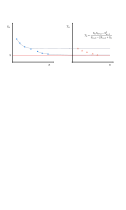
\includegraphics{figures/aitken}
  \caption{Geometrical interpretation of Aitken's \(\Delta^2\) method.}
  \label{fig:aitken}
\end{figure}

One can also show that if \((S_n)\) goes to its limit \(S\) at a rate strictly greater than \(1\)\footnote{$(S_{n})$, ${n \in \mathbb{N}}$ converges linearly to $S$ if there exists a number $\mu \in(0,1)$ such that \(\lim_{n \rightarrow \infty} \frac{\left|S_{n+1}-S\right|}{\left|S_{n}-S\right|}=\mu\).}, \((T_n)\) does not have a better rate of convergence.

In practice, the sequence produced by Aitken's \(\Delta^2\) method tends to converge faster to the limit than \((S_n)\) does.
Very often, it is much cheaper to calculate \((T_n)\), which involves only the calculation of differences, one multiplication, and one division, than to calculate many more terms of the sequence \((S_n)\).
Care must be taken, however, to avoid introducing errors due to insufficient precision when calculating the differences in the numerator and denominator of the expression.

There is, however, no universal sequence accelerator capable of accelerating all sequences.
It is also the case that nonlinear transformations can even fail to converge or converge to a value other than the limit of the original sequence \citep{brezinski_extrapolation_2013}.

According to \cite{brezinski_extrapolation_2013}, there is a very strong connection between sequence transformations and fixed point methods for solving \(x= g( x)\), \(g\colon \mathbb R\to \mathbb R\).
The most well-known example of this connection is that between Aitken's \(\Delta^{2}\) process and Steffensen's method.
\begin{equation}
T_{n}=S_{n}-\frac{\left(S_{n+1}-S_{n}\right)^{2}}{S_{n+2}-2 S_{n+1}+S_{n}}, \quad n=0,1, \ldots \quad\text{for Aitken's process}
\end{equation}
and
\begin{equation}
x_{n+1}=x_{n}-\frac{\left(g\left(x_{n}\right)-x_{n}\right)^{2}}{g\left(g\left(x_{n}\right)\right)-2 g\left(x_{n}\right)+x_{n}},\quad n=0,1, \ldots \quad\text{for Steffensen's method.}
\end{equation}

Turning to vector sequences and systems of nonlinear equations, let \(F:(\mathbf w^{k}) \to(\mathbf y^{k})\) be a vector extrapolation method defined by
\begin{equation}
\mathbf y^k = F\left(\mathbf w^{k}, \ldots, \mathbf w^{k+m}\right), \quad n=0,1, \ldots
\end{equation}
For solving the fixed point problem \(\mathbf x=\pazocal S(\mathbf x)\) one can associate to it the iterative method
\begin{equation}
\mathbf x^{k+1}=F\left(\mathbf x^{k}, \pazocal S(\mathbf x^{k}), \ldots, \pazocal S^{m}(\mathbf x^{k})\right), \quad n=0,1, \ldots
\end{equation}
where \(\pazocal S^{m+1}(\mathbf x)=\pazocal S \circ \pazocal S^{m}(\mathbf x)\) and \(\pazocal S^{0}(\mathbf x)=\mathbf x\).
This approach is called full cycling or simply cycling.
Conversely to any fixed point iteration of this form, one can associate a sequence transformation of the previous form.
See Box~\ref{box:vector_extrapolation_cycling} for the general algorithm, excluding the extrapolation method.

\begin{framedbox}[htbp]
  \caption{Timestep \(n\) of vector extrapolation with cycling.}
  \label{box:vector_extrapolation_cycling}
  \begin{center}
    \begin{minipage}{0.9\textwidth}
    \begin{enumerate}[(i)]
    \item Choose integers \(n\geq 0\) and \(k\leq 1\) and an initial vector \(\mathbf x^k =\mathbf x^*_0\).
    \item Compute \(\mathbf x^*_1\), \(\mathbf x^*_2\), \dots, \(\mathbf x^*_{n+k+1}\) via \(\mathbf x^*_{m+1} = \pazocal S(\mathbf x^*_m)\).
    \item Apply any of the four extrapolation methods, namely, MPE, RRE, MMPE, and SVD-MPE, to \(\mathbf x^*_n\), \(\mathbf x^*_{n+1}\), \dots, \(\mathbf x^*_{n+k+1}\), obtaining \(\mathbf s_{k,n}\).
    \item If \(\mathbf s_{n,k}\) satisfies the accuracy test, stop.\\
    Otherwise, set \(\mathbf x^*_0=\mathbf s_{n,k}\) and go to Step (ii).
    \end{enumerate}
    \end{minipage}
  \end{center}
\end{framedbox}

There is a variety of vector extrapolation methods, where the major two categories are polynomial methods and methods based on the \(\epsilon\)-algorithm \citep{brezinski_extrapolation_2013, sidi_vector_2017}.
In this presentation, only the first category is considered since the second requires a relatively large number of function evaluations per iteration, making it unsuitable for the present use-case \citep{sidi_vector_2017}.

\cite{sidi_vector_2017} presents four different polynomial extrapolation methods.
They all attempt to exprress the limit of the vector sequence as a linear combination of the \(p\) previous iterates, as follows
\begin{equation}
\mathbf s \approx \mathbf{s}_{k, m}=\sum_{j=0}^{m} \gamma_{j} \mathbf w^{k+j},
\end{equation}
where \(\mathbf s\) is the limit of the vector sequence.
The methods to be presented next appear naturally when considering the vector sequence generated by
\begin{equation}
  \mathbf w^{k+1} = \mathbf{T}\mathbf w^k +\mathbf d,
\end{equation}
where \(\mathbf I - \mathbf T\) is non-singular.
It is tighly connected to the solution of linear systems of equations.
Considering the minimal polynomial of \(\mathbf T\) with respect to \(\Delta \mathbf w^{k} = \mathbf w^{k+1} -\mathbf w^k\) and \(\boldsymbol \epsilon^k = \mathbf w^k - \mathbf s\)\footnote{A polynomial \(P(\lambda)\) is said to be minimal with respect to a vector \(\mathbf a\), if \(P(\mathbf T) \mathbf a = 0\) and it of least degree.}, \(P(\lambda)\),
\begin{equation}
  P(\lambda ) = \sum_{j=0}^i c_j \lambda^j, \quad c_i=1,
\end{equation}
where \(i\) is the degree of the polynomial, the limit of the sequence can be found exactly as
\begin{equation}
  \mathbf s = \frac{ \sum_{j=0}^i c_j \mathbf w^{k+j}}{ \sum_{j=0}^i c_j}.
\end{equation}

This can be derived considering the definition of \(P(\lambda)\), \(P(\mathbf T) \boldsymbol \epsilon^k=0\).
Therefore,
\begin{equation}
\mathbf 0=P(\mathbf T) \boldsymbol \epsilon^{k}=\sum_{j=0}^{i} c_{j} \mathbf T^{j}  \boldsymbol\epsilon^{j}=\sum_{j=0}^{i} c_{j} \boldsymbol \epsilon^{k+j}.
\end{equation}
and so
\begin{equation}
0=\sum_{i=0}^{k} c_{i} \boldsymbol{\epsilon}_{n+i}=\sum_{i=0}^{k} c_{i} \boldsymbol{x}_{n+i}-\left(\sum_{i=0}^{k} c_{i}\right) \mathbf{s}.
\end{equation}
Solving this for \(\mathbf s\), one obtains the desired result, provided \(\sum_{j=0}^{i} c_{j} \neq 0\).

The coefficients of \(P(\lambda)\) can be computed considering
\begin{equation}
\mathscr W^{i-1} \mathbf c^{\prime}=-\Delta \mathbf w_{k+i}, \quad \mathbf c^{\prime}=\left[c_{0}, c_{1}, \ldots, c_{i-1}\right]^{T},
\end{equation}
where \(\mathscr W^i = [\Delta \mathbf w^k, \dots, \Delta \mathbf w^{k+i}]\), since from the defintion of \(P(\lambda)\), one has
\begin{equation}
  \mathbf 0 = P(\mathbf T) \Delta \mathbf w^k = \sum_{j=0}^i c_i \mathbf T^j \Delta \mathbf w^k = \sum_{j=0}^i c_i \Delta \mathbf w^{k+j}.
\end{equation}

The degree of \(P(\lambda)\) can be as large as the dimension of \(\mathbf w\).
Hence, to be practical, the minimal polynomial extrapolation (MPE), the reduced rank extrapolation (RRE), the modified minimal extrapolation (MMPE), and the single-value decomposition, minimal polynomial extrapolation (SVD-MPE) all choose a polynomial of a lesser degree.
The approximations corresponding to each extrapolation method are presented in what follows.

\paragraph{MPE}

Solve the overdetermined linear system \(\mathscr W^{m-1} \mathbf c^{\prime}=-\Delta \mathbf w_{k+m}\) in the least-squares sense for \(\mathbf c^{\prime}=\left[c_{0}, c_{1}, \ldots, c_{m-1}\right]^{T}\).
This amounts to solving the optimization problem
\begin{equation}
\min _{c_{0}, c_{1}, \ldots, c_{p-1}}\left\|\sum_{j=0}^{m-1} c_{j} \Delta \mathbf w^ {k+j}+\Delta \mathbf w^{k+m}\right\|_2
\end{equation}
which can also be expressed as
\begin{equation}
  \min _{\mathbf c^{\prime}}\left\|\mathscr W^{m-1} \mathbf c^{\prime}+\mathbf w^{k+m}\right\|_2, \quad \mathbf c^{\prime}=\left[c_{0}, c_{1}, \ldots, c_{m-1}\right]^{T} .
\end{equation}
With \(c_{0}, c_{1}, \ldots, c_{k-1}\) available, set \(c_{m}=1\) and compute \(\gamma_{q}=c_{q} / \sum_{j=0}^{m} c_{j}, q=0,1, \ldots, m\), provided \(\sum_{j=0}^{m} c_{j} \neq 0\).

\paragraph{RRE}

Solve the overdetermined linear system \(\mathscr W^{m} \boldsymbol\gamma=0\) in the least-squares sense, subject to the constraint \(\sum_{j=0}^{m} \gamma_{j}=1\).
This amounts to solving the optimization problem
\begin{equation}
\min _{\gamma_{0}, \gamma_{1}, \ldots, \gamma_{m}}\left\|\sum_{j=0}^{m} \gamma_{j} \Delta\mathbf w^{k+j}\right\| \text { subject to } \sum_{j=0}^{m} \gamma_{j}=1
\end{equation}
which can also be expressed as
\begin{equation}
\min _{\boldsymbol\gamma}\left\|\mathscr W^{m} \boldsymbol\gamma\right\|_2 \quad \text { subject to } \sum_{j=0}^{m} \gamma_{j}=1 ; \quad \boldsymbol\gamma=\left[\gamma_{0}, \gamma_{1}, \ldots, \gamma_{m}\right]^{T} .
\end{equation}

\paragraph{MMPE}

Consider a set of \(m\) linearly independent vectors \(\mathbf q_j\), \(j=1, \dots, m\).
Solve the linear system
\begin{equation}
  \left(\mathbf q^{j}, \mathscr W^{m-1} \mathbf c^{\prime}\right)=-\left(\mathbf q^{j}, \Delta \mathbf w^{k+m}\right), \quad j=1, \ldots, m,
\end{equation}
which can also be expressed as
\begin{equation}
  \sum_{j=0}^{m-1}\left(\mathbf q_{j}, \Delta \mathbf w^{k+j}\right) \mathbf c_{j}=-\left(\mathbf q^{j}, \Delta \mathbf w^{k+p}\right), \quad j=1, \ldots, m.
\end{equation}
This is, in fact, a system of \(m\) linear equations for the \(m\) unknowns \(c_{0}, c_{1}, \ldots, c_{m-1}\).
With \(c_{0}, c_{1}, \ldots, c_{m-1}\) available, set \(c_{m}=1\) and compute \(\gamma_{q}=c_{q} / \sum_{j=0}^{m} c_{j}, i=0,1, \ldots, m\), provided \(\sum_{j=0}^{m} c_{j} \neq 0\).

\paragraph{SVD-MPE}

Solve the standard \(l_{2}\) constrained minimization problem
\begin{equation}
  \min_{\mathbf c}\left\|\mathscr W^{m} \mathbf c\right\|_{2} \quad \text { subject to }\|\mathbf c\|_{2}=1, \quad \mathbf c=\left[c_{0}, c_{1}, \ldots, c_{m}\right]^{T} .
\end{equation}
The solution \(\mathbf c\) is the right singular vector corresponding to the smallest singular value \(\sigma_{\min }\) of \(\mathscr W^{m}\), i.e., \({\mathscr W^{m}}^{*} \mathscr W^{m} \mathbf c=\sigma_{\min }^{2} \mathbf c\), \(\|\mathbf c\|_{2}=1\).
It is assumed that \(\sigma_{\min }\) is simple so that \(\mathbf c\) is unique up to a multiplicative constant \(\phi\), \(|\phi|=1\).

With \(c_{0}, c_{1}, \ldots, c_{m}\) available, compute \(\gamma_{q}=c_{q} / \sum_{j=0}^{m} c_{j}, q=0,1, \ldots, m\), provided \(\sum_{j=0}^{m} c_{j} \neq 0\).
The assumption that \(\sigma_{\min }\) is simple guarantees the uniqueness of the \(\gamma_{i}\).

When \(m=1\), MPE, RRE, MMPE, and SVD-MPE can be regarded as generalizations of the Aitken \(\Delta^2\)-process to the vector case.
Thus, when applied to the solution of a system of nonlinear equations using cycling
\begin{equation}
\mathbf{s}_{k, 1}=\begin{cases}
\mathbf x^{k}-\displaystyle\frac{\left(\Delta \mathbf x^{k}, \Delta \mathbf x^{k}\right)}{\left(\Delta \mathbf x^{k}, \Delta^{2} \mathbf x^{k}\right)} \Delta \mathbf x^{k} & \text { for MPE, } \\[10pt]
\mathbf x^{k}-\displaystyle\frac{\left(\Delta^{2} \mathbf x^{k}, \Delta\mathbf  x^{k}\right)}{\left(\Delta^{2} \mathbf x^{k}, \Delta^{2} \mathbf x^{k}\right)} \Delta \mathbf x^{k} & \text { for RRE, } \\[10pt]
\mathbf x^{k}-\displaystyle\frac{\left(\mathbf  q_{1}, \Delta \mathbf x^{k}\right)}{\left(\mathbf  q_{1}, \Delta^{2} \mathbf  x^{k}\right)} \Delta \mathbf x^{k} & \text { for MMPE, } \\[10pt]
\mathbf x^{k}-\displaystyle\frac{\left(\mathbf g_{0}, \Delta\mathbf x^{k}\right)}{\left( \mathbf g_{0}, \Delta^{2} \mathbf x^{k}\right)} \Delta \mathbf  x^{k} & \text { for SVD-MPE. }
\end{cases}
\end{equation}

\cite{sidi_vector_2017} also suggest cycling with frozen \(\gamma_i\), where after some iterations the \(\gamma_i\) are frozen and reused henceforth.
A parallel version of the full cycling procedure is also described.

\paragraph{Connection to Krylov subspace methods}

According to \cite{sidi_vector_2017}, the so-called Krylov subspace methods are closely related to the vector extrapolation methods presented above.
When the latter is applied to vector sequences obtained using fixed-point iterative methods to nonsingular linear systems of equations, they are mathematically equivalent.
More precisely, the MPE and the RRE methods are mathematically equivalent to the methods of Arnoldi and generalized minimal residual (GMR).

However, Krylov subspace methods and extrapolation methods differ in their algorithmic aspects entirely:
The only input of the former is a procedure that performs the matrix-vector multiplication without explicitly knowing the matrix coefficient matrix.
The latter takes as their only input a vector sequence that results from a fixed-point iterative scheme without knowing the matrix coefficient.

In \cite{michler_interface_2005}, a Krylov-subspace method is proposed in the context of FSI.
However, as pointed out by \cite{kuttler_vector_2009}, the correct term for this approach should be instead a "Krylov-based vector extrapolation" method.
The method proposed can be obtained by applying the RRE to the sequence of residuals computed as
\(\Delta \mathbf r^*_i = \mathbf x^*_i - \mathbf x^k\), where the subscript \(i\) concerns the internal loop of the vector extrapolation method, and whose limit is \(\mathbf 0\).
\cite{kuttler_vector_2009} argues that these residual differences have unfavorable numerical properties and should be avoided.


% \Floatbarrier

\section{Multipoint iteration functions with memory}

Multipoint iteration functions are rarer and are not thoroughly investigated in this exposition.
One can mention the Eirola-Nevanlinna family of methods \citep{fang_two_2009} and Netwon-Krylov method that reuses the Krylov subspace from previous iterations \citep{sidi_vector_2017}.

\section{Summary}

The overview provided in this chapter centered on implicit techniques for partitioned multi-physics coupled applications.
The problem can be slightly reformulated as a system of nonlinear equations, where the residual represents the difference between the input and output after the fixed-point procedure has been applied.
This allows the problem to be solved using a variety of methods described in the literature to tackle system of nonlinear equations.
The key issues in the current application are the memory requirements of the numerical technique due to a potential high number of unknowns and the number of residual evaluations, as each assessment necessitates a significant computational effort.
Table~\ref{tab:mem_nr_func_eval_obs} provides information on the memory requirements, the number of function evaluations per nonlinear iteration, and some pertinent observations for each technique under consideration.

Except for the MMPE and SVD-MPE approaches, the computational performance of all the methods discussed in the present chapter are analyzed in the next chapter (Chapter~\ref{ch:val_acc_techniques}).
As seen in Table~\ref{tab:form_nonlin_methods}, where the update formulae for the methods are compiled, their implementation is made simpler by the similarities in the update formula for the value of the unknown variable at each nonlinear iteration.


\begin{landscape}
\begin{table}[htbp]
  \caption{Summary of the comparison between method for the solution methods of non-linear systems of equations. \(n\) here denotes the number of unknowns and \(m\) denotes depending on the context the number of previous iterates considered, the number of fixed point evaluations or the size of the Krylov subspace.}
\label{tab:mem_nr_func_eval_obs}
  % \setlength{\tabcolsep}{1pt}
  \centering
    \begin{tabular}{l cc p{10.5cm}}
    Method & \makecell[c]{Memory\\requirements} & \makecell[c]{Nr function\\evaluations\\per iteration} & Observations\\
    \hline  \hline
    \multirow{3}{*}{\vphantom{\Big|}Fixed-point iteration} & \multirow{3}{*}{2 \((n\times 1)\) vectors} & \multirow{3}{*}{1} & \textbullet Often diverges.\\
    & & &\textbullet Simplest method.\\
    & & &\textbullet Memory efficient.\\
    \hline
    \multirow{3}{*}{Underrelaxation} & \multirow{3}{*}{2 \((n\times 1)\) vectors} & \multirow{3}{*}{1} & \textbullet Simple.\\
    & & &\textbullet Improved stability over fixed-point.\\
    & & &\textbullet Need to manually choose a relaxation parameter.\\
    \hline
    \multirow{3}{*}{Aitken relaxation} & \multirow{3}{*}{3 \((n\times 1)\) vectors} & \multirow{3}{*}{1} & \textbullet Very popular in FSI.\\
    & & & \textbullet Dynamic relaxation.\\
    & & & \textbullet Improved stability over fixed-point.\\
    \hline
    \multirow{3}{*}{\makecell[l]{Broyden-like family\\\citep{fang_two_2009}}} & \multirow{3}{*}{\makecell[c]{2 \((n\times 1)\) vectors\\2 \((n\times (m-1))\) matrices}} & \multirow{3}{*}{1} & \textbullet \(\pazocal O(nm^2)\) computation complexity (\(QR\) decomposition). \\
    & & & \textbullet Low number of function evaluations\\
    & & & \textbullet Superlinear convergence when \(m=1\).\\
    \hline
    \multirow{3}{*}{\makecell[l]{Broyden's method\\\citep{kelley_solving_2003}}} & \multirow{3}{*}{\makecell[c]{Up to\\ \((m+2) (n\times 1)\) matrices}} & \multirow{3}{*}{1} & \textbullet \(\pazocal O(n)\) computation complexity.\\
    & & & \textbullet Low storage.\\
    & & & \textbullet Superlinear convergence.\\
    \hline
    \multirow{3}{*}{Newton-Krylov} & \multirow{3}{*}{\makecell[c]{Up to\\\((m+1)\) \((n\times 1)\) vectors}} & \multirow{3}{*}{\(m+1^*\)} & \textbullet Large number of iterations possible.\\
    & & & \textbullet Popular for the solution of systems of nonlinear equations.\\
    & & & \textbullet Quadratic convergence under appropriate conditions.\\
    \hline
    \multirow{2}{*}{\makecell[l]{Vector extrapolation\\ in cycling mode}} & \multirow{2}{*}{\((m+2)\) \((n\times 1)\) vectors} & \multirow{2}{*}{\(m+1\)} & \textbullet Large number of function evaluations.\\
    & & & \textbullet \(\pazocal O(nm^2)\) computational complexity (\(QR\) decomposition).\\
  \hline\hline
  \multicolumn{4}{l}{\vphantom{\Huge |}\parbox{\textwidth}{\footnotesize{  \(^*\) The number of function evaluations in the Newton-Krylov methods will depend on how many iterations it will take for the inner loop to converge. There is a function evaluation per iteration of the inner loop.}}}
  \end{tabular}
\end{table}
\end{landscape}



\begin{table}[htbp]
  \caption{Summary of the update formulas for the solution methods of non-linear systems of equations.}
\label{tab:form_nonlin_methods}
  % \setlength{\tabcolsep}{1pt}
  \centering
    \begin{tabular}{l c}
    Method & Update formula\\
    \hline\hline
    \vphantom{\Huge |}Fixed-point &  \makecell[l]{\(\mathbf x^{k+1} = \mathbf x^k -  \pazocal R^k\)}\\
    \hline
    Underrelaxation & \makecell[l]{\vphantom{\Huge |}\(\mathbf x^{k+1} = \mathbf x^k - \omega\pazocal R^k\),\\\(0<\omega<1\).}\\
    \hline
    Aitken relaxation & \makecell[l]{\vphantom{\Huge |}\(\mathbf x^{k+1} = \mathbf x^k - \omega^{(k)}\pazocal R^k\),\\    \(\omega^{(k)}=-\omega^{(k-1)} \displaystyle\frac{\left(\mathbf{r}^{(k)}-\mathbf{r}^{(k-1)}\right)^{\mathrm{T}} \mathbf{r}^{(k-1)}}{\left(\mathbf{r}^{(k)}-\mathbf{r}^{(k-1)}\right)^{2}}.\)
    }\\
    \hline
    Broyden's family & \makecell[l]{\vphantom{\Huge |} \(\mathbf x^{k+1} = \mathbf x^{k}- \left(G_\pazocal R^{k-m} +\left(\mathscr{X}^{k}-G_\pazocal R^{k-m} \mathscr{R}^{k}\right){\mathbf V^k}^T\right) \pazocal R^k,\)\\
    \({\mathbf V^k}^T = {\mathbf M^k}^{-1}{\mathbf N^k}^T\),\\
    Type I:  \({M^k} = {\mathscr X^k}^T G_\pazocal R^k \mathscr R^k,\quad {N^k}^T = {\mathscr X^k}^T G_\pazocal R^k,\)\\
    Type II: \({M^k} = {\mathscr R^k}^T \mathscr R^k,\quad {N^k}^T = {\mathscr R^k}^T\)\\
    {\small \(\mathbf V^k\) is usually computed using \(QR\)-decomposition.}
    }\\
    \hline
    Anderson's family & \makecell[l]{\vphantom{\Huge |} \(\mathbf x^{k+1} = \mathbf x^{k} -\left(-\beta \mathbf I+\left(\mathscr{X}^{k}+\beta \mathscr{R}^{k}\right){\mathbf V^k}^T\right) \pazocal R^k,\)\\
    \({\mathbf V^k}^T = {\mathbf M^k}^{-1}{\mathbf N^k}^T\),\\
    Type I:  \({M^k} = {\mathscr X^k}^T \mathscr R^k,\quad {N^k}^T = {\mathscr X^k}^T ,\)\\
    Type II: \({M^k} = {\mathscr R^k}^T \mathscr R^k,\quad {N^k}^T = {\mathscr R^k}^T\)\\
    {\small \(\mathbf V^k\) is usually computed using \(QR\)-decomposition.}
    }\\
    \hline
    Newton-Krylov & \makecell[l]{\vphantom{\Huge |} \(\mathbf x^{k+1} = \mathbf x^{k} +\Delta \mathbf x^k\)\\
    \(J_\pazocal R(\mathbf x^k)\Delta x^k = -\pazocal R^k\) solved using a Krylov method\\
    to accuracy \(  \|J_\pazocal R(\mathbf x^k) \Delta x^*_m+ \pazocal R(\mathbf x^k)\| \leq \eta\|\pazocal R(\mathbf x^k)\|\)}
    \\
    \hline
    \makecell[l]{Vector extrapolation\\ in cycling mode} & \makecell[l]{\vphantom{\Huge |}
    \(\mathbf x^{k+1} = \sum_{j=0}^m \gamma_j \pazocal S^{i+j}(\mathbf x^k)\),\\
    \(\gamma_q = c_q/\sum_j c_j,\quad q=0,1,\dots,m,\)\\
    \textbf{MPE}: \(\mathbf c ' = [c_0,c_1,\dots,c_{m-1}]^T = \arg \min_{\bar{\mathbf c}} \left\|\mathscr S^{m-1} \bar{\mathbf c}^\prime + \pazocal S^{i+m}(\mathbf x^k)\right\|_2\),\\
    \(c_m=1\),\\
    \textbf{RRE}: \(\boldsymbol{\gamma} = [\gamma_0,\gamma_1,\dots,\gamma_{m}]^T = \arg \min_{\bar{\boldsymbol{ \gamma}}} \left\|\mathscr S^{m} \hat{\boldsymbol{\gamma}}\right\|_2\),\\
    Subject to \(\sum_{j=0}^m \gamma_j =1\).\\
    \textbf{MMPE}: \(\left(\mathbf q^{j}, \mathscr S^{m-1} \mathbf c^{\prime}\right)=-\left(\mathbf q^{j}, \pazocal S^{i+m}(\mathbf x^k)\right), \quad j=1, \ldots, m,\)\\
    for a set of \(m\) linearly independent vectors \(\mathbf q_j\), \(j=1, \dots, m\).\\
    \(\mathbf c ' = [c_0,c_1,\dots,c_{m-1}]^T.\)\\
    \textbf{SVD-MPE}: \(\mathbf c = \arg\min_{\bar{\mathbf c}}\left\|\mathscr S^{m} \bar{\mathbf c}\right\|_{2} \quad \text { subject to }\|\bar{\mathbf c}\|_{2}=1,\)\\
    \(\mathbf c=\left[c_{0}, c_{1}, \ldots, c_{m}\right]^{T}\).
    }\\
  \hline\hline
  \end{tabular}
\end{table}

\FloatBarrier

\newpage\null\thispagestyle{blank}\newpage

% \include{conclusions}
\appendix
% \include{annex}

\bibliography{Thermomechanics.bib}

\end{document}
